% zu sagen:
% alle Exerpte aus Bd 1 = 1669
% VII,2-Editiion bringt nur etwa die Hälfte des Textbestandes; Ausgelassenes im Text nur an einer Stelle gekennzeichne
% \input{gesamttex/edit/LH035_14_02_152v.tex}
\begin{ledgroupsized}[r]{120mm}
\footnotesize 
\pstart 
\noindent\textbf{\"{U}berlieferung:} 
\pend
\end{ledgroupsized}
\begin{ledgroupsized}[r]{114mm}
\footnotesize 
\pstart \parindent -6mm
\makebox[6mm][l]{\textit{L}}%
Auszüge mit Bemerkungen aus \cite{00044}\textsc{H. Fabri}, \textit{Physica, id est scientia rerum corporearum in decem tractatus distributa}, Bd. 1, Lyon 1669: LH XXXV 14, 2 Bl. 135, 138-158.
9~Bog. und 4 Bl. 2\textsuperscript{o}. 24 S. zweispaltig (mit Ausnahme von Bl. 151 r\textsuperscript{o} und 152 v\textsuperscript{o}) beschrieben.
% Aus Bl. 139, 146 und 157 St\"{u}cke von der Breite einer Spalte herausgeschnitten. Die L\"{a}nge des Ausschnitts betr\"{a}gt f\"{u}r Bl. 139 etwa 4/5 der Seitenl\"{a}nge und f\"{u}r die beiden anderen Bl\"{a}tter etwa 1/6 der Seitenl\"{a}nge.
Textfolge:
Bl.~152~v\textsuperscript{o}, 151~r\textsuperscript{o}, 154~v\textsuperscript{o}, 153~r\textsuperscript{o}, 155~r\textsuperscript{o}, 156~r\textsuperscript{o}, 157~v\textsuperscript{o}, 150~v\textsuperscript{o}, 149~r\textsuperscript{o}, 147~r\textsuperscript{o}, 148~r\textsuperscript{o}, 148~v\textsuperscript{o}, 146~r\textsuperscript{o}, 146~v\textsuperscript{o}, 145~v\textsuperscript{o}, 144~r\textsuperscript{o}, 144~v\textsuperscript{o}, 143~v\textsuperscript{o}, 142~r\textsuperscript{o}, 141~v\textsuperscript{o}, 140~r\textsuperscript{o}, 139~v\textsuperscript{o}, 138~r\textsuperscript{o}, 158~v\textsuperscript{o}.
Auf Bl. 135~r\textsuperscript{o} nur Leibniz' eigenhändige Aufschrift: \textit{Excerpta philosophica.}
Die übrigen Seiten sind leer.
Bl. 136-137 überliefern das Stück \cite{01120}\textit{LSB} VI, 2 N.~39\textsubscript{2} (Auszüge mit Bemerkungen aus \cite{00043}\textsc{H. Fabri}, \textit{Tractatus duo: quorum prior est de plantis et de generatione animalium; posterior de homine}, Paris 1666).
Sämtliche Texttr\"{a}ger sind in den Bogen eingeschlagen, der Bl. 135~r\textsuperscript{o} umfasst.
% Die folgenden S. sind leer: Bl.~152~r\textsuperscript{o}, 151~v\textsuperscript{o}, 154~r\textsuperscript{o}, 153~v\textsuperscript{o}, 155~v\textsuperscript{o}, 156~v\textsuperscript{o}, 157~r\textsuperscript{o}, 150~r\textsuperscript{o}, 149~v\textsuperscript{o}, 147~v\textsuperscript{o}, 145~r\textsuperscript{o}, 143~r\textsuperscript{o}, 142~v\textsuperscript{o}, 141~r\textsuperscript{o}, 140~v\textsuperscript{o}, 139~r\textsuperscript{o}, 138~v\textsuperscript{o}, 158~r\textsuperscript{o}.
% Die Exzerpte und Kommentare zum 9. Traktat von Fabris \title{Physica} stehen auf Bl. 136-137 und sind in \textit{LSB} VI, 2, N. $39_2$ erschienen.
% Auf Bl. 135 r\textsuperscript{o} die Notiz: \textit{Excerpta philosophica.} R\"{u}ckseite leer. In den zugeh\"{o}rigen Bogen sind die Textr\"{a}ger unseres St\"{u}cks eingeschlagen.
Urspr\"{u}nglich war das Papier tlw. f\"{u}r das \title{Corpus juris reconcinnatum}\cite{01000} vorgesehen (vgl. hierzu \textit{LSB} VI, 2, S.~XXI\,f.).
Dies entnimmt man den an verschiedenen Stellen des Ms. notierten Gesetzesanf\"{a}ngen aus dem zweiten Teil des \textit{Corpus juris civilis}.
Dabei handelt es sich um Merkzeichen in meist abgek\"{u}rzter Form, die von Leibniz beim Exzerpieren nicht getilgt, sondern \"{u}ber- bzw. umschrieben wurden.
Sie werden im Folgenden nicht wiedergegeben% , da sie offenbar nur eine mnemotechnische Funktion hatten
.\\%
Cc 2, Nr. 00
\pend
\end{ledgroupsized}
%
\begin{ledgroupsized}[r]{114mm}
\footnotesize 
\pstart \parindent -6mm
\makebox[6mm][l]{\textit{E}}%
(tlw.) \cite{01120}\title{LSB} VI, 2 N. $39_1$. % /S. 186-209.
\pend
\end{ledgroupsized}
%\normalsize
\vspace*{5mm}
\begin{ledgroup} 
\footnotesize 
%
\count\Afootins=1200
\count\Bfootins=1200
\count\Cfootins=1200
\pstart
\noindent\footnotesize{\textbf{Datierungsgr\"{u}nde:}
Die Datierung von \cite{01120}\title{LSB} VI, 2 N. $39_1$ wird übernommen (für die Begründung siehe dort, S. 186f.).
% Leibniz hat in einem Brief an Martin Fogel vom Januar 1671 das Erscheinen der ersten beiden Teile (1669, 1670) der \title{Physica}\cite{00044} Honor\'{e} Fabris erw\"{a}hnt (\title{LSB} II, 1 N. 38). Auf diesen Titel wird dar\"{u}ber hinaus mehrmals in der \title{Hypothesis physica nova}\cite{00256} Bezug genommen. Insbesondere diskutiert Leibniz die bei Experimenten mit Lacrymae vitreae auftretenden Ph\"{a}nomene in einer Weise, die eine Vetrautheit mit Fabris Ansichten erkennen lassen. Die entsprechenden Passagen im Appendix zu Buch 5 des 1. Traktats der Physik werden in dem vorliegenden St\"{u}ck ausf\"{u}hrlich exzerpiert. Eine Entstehungszeit der Exzerpte zwischen Herbst 1670 und Fr\"{u}hjahr 1671 ist daher sehr wahrscheinlich. Die Datierung k\"{o}nnte dadurch in Zweifel gezogen werden, dass Leibniz sein Handexemplar der Fabrischen Physik erst im Januar 1672 erhalten hat. Eine Sichtung der Anstreichungen und Randbemerkungen in \title{LSB} VI, 2 N. 39.3, wo die Marginalien gedruckt sind, zeigt allerdings, dass sich diese ausschlie{\ss}lich auf Passagen der Physik beziehen, zu denen keine Exzerpte vorliegen. Die Marginalien komplettieren daher die vermutlich 1670 beginnende Lekt\"{u}re zu einem sp\"{a}teren Zeitpunkt. Wir folgen daher nicht den Bearbeitern von \title{LSB} VI, 2 N. 39.1, die eine Entstehungszeit der Exzerpte zwischen Herbst 1670 und Fr\"{u}hjahr 1672 annehmen.
}
\pend
\end{ledgroup}
%
\vspace*{8mm}
\pstart 
\normalsize
\noindent[152~v\textsuperscript{o}] 
\textit{Physica\protect\index{Sachverzeichnis}{physica} id est Scientia Rerum Corporearum in decem Tractatus distributa,} auctore \textso{Honorato Fabri }\protect\index{Namensregister}{\textso{Fabri}, Honor\'{e} SJ 1607-1688}\textit{Soc. Jesu. Nunc primum in lucem prodit Lugduni sumtibus Laurentii Anisson 1669. 4\textsuperscript{o}. cum privilegio} \edtext{\textit{Regis.}}{\lemma{\textit{Regis.}}\Cfootnote{\textsc{H. Fabri}, \title{Physica}\cite{00044}, Bd.~1, Lyon 1669, Titelkupfer.}} Dedicat Leopoldo\protect\index{Namensregister}{\textso{Leopoldo dei Medici}, Kardinal 1617-1675} magni Hetruriae ducis fratri Cardinali. In praefatione ait ultimum jam tractatum physicae olim a se editum. Partes operis ita enumerat: decem se composuisse tractatus, \textit{quatuor esse de statibus corporum sensibilibus, unum de principiis corporis naturalis, generatione et corruptione ejusdem et quatuor elementis, duos de mixtione et mixtis imperfectis et perfectis ut vocant; de corpore coelesti\protect\index{Sachverzeichnis}{corpus coelestis} unum, duos de plantis animalibus et} \edtext{\textit{homine.}}{\lemma{\textit{homine.}}\Cfootnote{H. \textsc{Fabri}, \title{Physica}\cite{00044}, Bd. 1, Lyon 1669, Praefatio, Nr.~1.}} \textso{Primo }tractatu se dicere de \textit{corpore quanto, de tenso et presso, raro et denso, gravi et levi, opaco et} \edtext{\textit{diaphano.}}{\lemma{\textit{diaphano.}}\Cfootnote{a.a.O.\cite{00044}, Nr.~1.}}
Tractatu \textso{secundo:}
\textit{de calido et frigido, lucido et illuminato, humido, sicco, duro, molli, tenui crasso, et multis aliis corporum statibus\protect\index{Sachverzeichnis}{status corporum}, qui sub sensus} \edtext{\textit{cadunt,}}{\lemma{\textit{cadunt,}}\Cfootnote{a.a.O.\cite{00044}, Nr.~1.}} ut et corporum resistentia\protect\index{Sachverzeichnis}{resistentia corporum}. In \textso{tertio} fuse et \textit{accurate de coloribus\protect\index{Sachverzeichnis}{color} et} \edtext{\textit{sonis\protect\index{Sachverzeichnis}{sonus}.}}{\lemma{\textit{sonis.}}\Cfootnote{a.a.O.\cite{00044}, Nr.~1.}} In \textso{quarto} de \textit{odoribus\protect\index{Sachverzeichnis}{odor} et saporibus\protect\index{Sachverzeichnis}{sapor}, de alteratione, reflexione qualitatum\protect\index{Sachverzeichnis}{alteratio qualitatum} et refractione in}
\textit{\textso{quinto}}
\textit{de generatione corporis physici\protect\index{Sachverzeichnis}{generatio corporum} et principiis utriusque nec non de 4} \edtext{\textit{Elementis\protect\index{Sachverzeichnis}{elementa}.}}{\lemma{\textit{Elementis.}}\Cfootnote{a.a.O.\cite{00044}, Nr.~1.}} In \textso{6}\textsuperscript{to} \textit{de mixtione\protect\index{Sachverzeichnis}{mixtio} in genere et mixtis imperfectis quibuslibet, igneis scilicet, aqueis aeris et} \edtext{\textit{terrestribus;}}{\lemma{\textit{terrestribus;}}\Cfootnote{a.a.O.\cite{00044}, Nr.~1.}} in \textso{7}\textsuperscript{mo} \textit{de mixtis perfectis, metallis\protect\index{Sachverzeichnis}{metalla} scilicet lapidibus\protect\index{Sachverzeichnis}{lapis} et succis; in octavo de corpore coelesti\protect\index{Sachverzeichnis}{corpus coelestis}, nimirum de planetis\protect\index{Sachverzeichnis}{planeta}, stellis\protect\index{Sachverzeichnis}{stella}, cometis\protect\index{Sachverzeichnis}{cometa}, corporum coelestium motibus\protect\index{Sachverzeichnis}{motus corporum coelestium}, et communi medio\protect\index{Sachverzeichnis}{medium communis}, nonum jam dedimus, qui est de plantis\protect\index{Sachverzeichnis}{planta} et generatione animalium\protect\index{Sachverzeichnis}{generatio animalium}, et ultimum qui est de} \edtext{\textit{homine\protect\index{Sachverzeichnis}{homo}.}}{\lemma{\textit{homine.}}\Cfootnote{a.a.O.\cite{00044}, Nr.~1.}} Cartesium\protect\index{Namensregister}{\textso{Descartes} (Cartesius, des Cartes), Ren\'{e} 1596-1650} sugillat tecto nomine, finxisse sibi potius mundum \edtext{quam praesentem}{\lemma{quam}\Bfootnote{\textit{(1)}\ qualis est \textit{(2)}\ praesentem \textit{L}}} illustrasse, Democrito\protect\index{Namensregister}{\textso{Demokrit} von Abdera 2.H. 5. Jh. v. Chr.} suo similes, qui ut \edtext{res\protect\index{Sachverzeichnis}{res visibiles} visibiles}{\lemma{res}\Bfootnote{\textit{(1)}\ seu \textit{(2)}\ visibiles \textit{L}}} melius cerneret, \textit{oculos\protect\index{Sachverzeichnis}{oculi} ut ajunt sibi eruendos} \edtext{\textit{putavit.}}{\lemma{\textit{putavit.}}\Cfootnote{a.a.O.\cite{00044}, Nr.~3.}}
Quaeritur ab Arabibus\protect\index{Sachverzeichnis}{Arabes} depravatum ad nos Aristotelis\protect\index{Namensregister}{\textso{Aristoteles}, 384-322 v. Chr.} sensum pervenisse. \edtext{Ignatium jussisse Aristotelem\protect\index{Namensregister}{\textso{Aristoteles}, 384-322 v. Chr.} in quantum a fide non deviaret, Averroem\protect\index{Namensregister}{\textso{Averro\"{e}s } (Ibn Roschd) 1126-1198} minime sequerentur}{\lemma{}\Bfootnote{Ignatium\protect\index{Namensregister}{\textso{Ignatius von Loyola} 1491-1556} jussisse [...] minime sequerentur. \textit{erg.} \textit{L}}} \hspace{-1.2mm}\edtext{.}{\lemma{sequerentur.}\Cfootnote{a.a.O.\cite{00044}, Nr.~9.}}
\pend 
\pstart Honorat. Fab. praef. tract. prim. \textit{Phys.} num. 5. Si ampullam vitream\protect\index{Sachverzeichnis}{ampulla vitrea} longioris et angustioris colli \textit{in quam aqua infusa est ad datam altitudinem in calidam immergas aqua} \edtext{\textit{subsidit}}{\lemma{\textit{subsidit}}\Cfootnote{a.a.O.\cite{00044}, Nr.~5.}}, si in gelidam sive \textit{nivatam} \edtext{\textit{ascendit.}}{\lemma{\textit{ascendit.}}\Cfootnote{a.a.O.\cite{00044}, Nr.~5.}} Contra accipe phialam (+ NB +) concavam\protect\index{Sachverzeichnis}{phiala concava} exterius et convexam\protect\index{Sachverzeichnis}{phiala convexa} interius, \textit{prior enim pro more ampullarum exterius convexa} \edtext{\textit{est;}}{\lemma{\textit{est;}}\Cfootnote{a.a.O.\cite{00044}, Nr.~5.}} et sic immerge, ascendet aqua\protect\index{Sachverzeichnis}{aqua calida} in calido, descendet in frigido. Hinc concludit oriri hoc non ex contentis in phiala, sed figura vitri. Nam vitrum rarescere calore in ampulla priore extrorsum, ita aqua subsidit, in posteriore introrsum, ita aqua ascendit; densari frigore illi introrsum hinc ascensus; hic extrorsum hinc \edtext{descensus.}{\lemma{descensus.}\Cfootnote{a.a.O.\cite{00044}, Nr.~5.}} Adde aliud experimentum, accipe arcum vitreum tensum, \textit{cujus extremitates fidicula tensa adducantur, ubi arcus calescit atque rarescit, magis explicatur arcus et fidicula} \edtext{\textit{tenditur}}{\lemma{\textit{tenditur}}\Cfootnote{a.a.O.\cite{00044}, Nr. 6.}}, hinc sonat acutius, in frigido gravius, quippe arcu laxato.\pend 
\pstart \textso{Honor. Fab. phys. tract. 1. praef. num. 12.} \textit{Aer\protect\index{Sachverzeichnis}{aer in tubo} triginta digitorum altitudinis in tubo ad digitalem} \edtext{\textit{molem}}{\lemma{\textit{molem}}\Cfootnote{a.a.O.\cite{00044}, Nr. 12.}} contrahi potest.\pend 
\pstart \textso{Honor. Fab. phys. tract. 1. praef. num. 15.} \textit{Forma etiam dicitur species ratio, actus, quae est ut ordo numerus Musica\protect\index{Sachverzeichnis}{musica} etc. ac proinde respectus et relatio (de forma materiali loquor) hinc seorsum a materia esse vel concipi nequit hinc dicitur educi e potentia materiae hinc cum speciem constituat ab alia forma solo numero non differt cum eadem forma sit, id est eadem ratio, qua ignis\protect\index{Sachverzeichnis}{ignis} A ignis est, et ignis B, hinc forma non dicitur produci, aut} \edtext{\textit{generari.}}{\lemma{\textit{generari.}}\Cfootnote{a.a.O.\cite{00044}, Nr. 15.}}
\pend 
\pstart \textso{Honor. Fab. phys. tract. 1. praef. num. 19.} Aristoteles\protect\index{Namensregister}{\textso{Aristoteles}, 384-322 v. Chr.} statuit, ut terram absolute gravem, ita ignem absolute \edtext{levem,}{\lemma{levem,}\Cfootnote{\textsc{Aristoteles}, \title{De caelo}\cite{00303} IV 4, 311a.}} putat enim corpus leve propria vi assurgere \textit{ex minus probatis experimentis, quod nimirum per medium aquam major aeris moles velocius ascendat quam minor, item ex falsa hypothesi coeli solidi, in quibus ab eo} \edtext{\textit{discedimus.}}{\lemma{\textit{discedimus}.}\Cfootnote{\textsc{H. Fabri}, \title{Physica}\cite{00044}, Bd. 1, Lyon 1669, Praefatio, Nr. 19.}}
\pend 
\pstart \textso{Honor. Fab. phys. tract. 1. praef. num.} \edtext{[\textso{21}]}{\lemma{}\Bfootnote{\textso{22}\textit{\ L \"{a}ndert Hrsg.}}}\textso{.} \textit{Finis et forma quasi unum quoddam existimanda sunt, observamus autem vix}
\textit{philosophum cogitasse de ullo effectu absoluto qui a dictis 4 causarum generibus producatur; ubi enim fabricatur domus, aut fit statua, qui quaeso absolutus effectus de novo est, id est per veram actionem producitur? nullus omnino. Ita prorsus in generatione plantae aut bruti, nulla Entitas absoluta de novo est, ipsa enim forma mera est relatio, id est ratio, qua hoc vel illud est, quae revera non producitur ut suo loco demonstrabimus: in hominis generatione aliquid de novo est, praeter Ens respectivum\protect\index{Sachverzeichnis}{ens respectivum}, nimirum anima rationalis\protect\index{Sachverzeichnis}{anima rationalis}, sed haec a DEo non a generante} \edtext{\textit{producitur.}}{\lemma{\textit{producitur}.}\Cfootnote{a.a.O.\cite{00044}, Nr. 21.}}
\pend 
\pstart \textso{Honor. Fab. phys. tract. 1. praef. n. 26.} Quantitatem non esse Entitatem quandam \edtext{absolutam.}{\lemma{absolutam.}\Cfootnote{a.a.O.\cite{00044}, Nr. 26.}}
\pend
\pstart \textso{Honor. Fab. phys. tract. 1. praef. n. 26.}
\textit{Quid in Logicis praestiterim illi revera sciunt, qui meam Analyticen cum Analyticis prioribus conferre dignati fuerunt, cum enim omnia satis confuse demonstrata licet accuratissime apud}
\textit{Aristotelem}\protect\index{Namensregister}{\textso{Aristoteles}, 384-322 v. Chr.}
\textit{legerentur, idque uno tenore absque ulla propositionum fibula aut theorematum serie, in multa distinxi propositionum centena et forte millena praemissis definitionibus et axiomatis more geometrico\protect\index{Sachverzeichnis}{more geometrico}, et cum aliqua deessent de meo supplevi praesertim de artificio consequentiae enthymematis syllogisimi hypothetici, disjunctivi, \edtext{copulativi.}{\lemma{copulativi.}\Cfootnote{a.a.O.\cite{00044}, Nr. 26.}}}
[151~r\textsuperscript{o}]
\pend%
\count\Afootins=1000
\count\Bfootins=1000
\count\Cfootins=1000
\pstart%
%
%
%
% \input{gesamttex/edit/LH035_14_02_151r.tex}
% [151~r\textsuperscript{o}]
\textso{Honor. Fab. Phys. tract. 1. praefat. num. 27. sqq.} \textit{In Metaphysica\protect\index{Sachverzeichnis}{metaphysica} rationes universales\protect\index{Sachverzeichnis}{rationes universales} discussi earumque proprietates 
\edtext{demonstravi}{\lemma{\textit{demonstravi}}\Cfootnote{\textsc{H. Fabri, }\cite{01045}\textit{Metaphysica demonstrativa, sive scientia rationum universalium}, Lyon 1648.}}} (+ ni fallor Mousnerius\protect\index{Namensregister}{\textso{Mousnerius}, Petrus} adjutor +) ordine rebus congruo, etsi enim universalis ratio sit quae corpori et incorporeo competit, dantur tamen gradus universalitatis, \textit{v.g. ratio objectiva omnium universalissima est, cum Enti, non Enti, universalibus et singularibus competat, tum ratio universalis, ratio Entis absoluti respectivi, ratio substantiae accidentis,} multam forte iis lucem attulimus quae Aristoteles\protect\index{Namensregister}{\textso{Aristoteles}, 384-322 v. Chr.} confuse, et saepe repetita prolixis cum prooemiis tradidit. Verum objectum igitur scientiae statui rationem universalem ejusque \textit{16 capita}, quia
\textit{totidem subjecta universalia, quorum proprietates praemissis definitionibus et axiomatis more geometrico demonstravi.} Doctrinam de \textit{DEo et Angelis} a Metaphysica \edtext{rescidi.}{\lemma{rescidi.}\Cfootnote{H. \textsc{Fabri}, \title{Physica}\cite{00044}, Bd. 1, Lyon 1669, Praefatio, Nr.~27.}} Tractatus meus \textit{de motu locali\protect\index{Sachverzeichnis}{motus localis} \edtext{corporum}{\lemma{corporum}\Cfootnote{\textsc{H. Fabri,}\title{ Tractatus physicus de motu locali}, Lyon 1646\cite{00307}}} a multis annis juxta meam hypothesin in publicam lucem editus multa nova continet.} Edidimus et dialogos, puta in prima parte dialogorum physicorum, multa dixi de motu, sed potissimum in secunda in qua multos dialogos habes de motu locali. \textit{Omnia} nostra (+ physica +) \textit{in grande volumen congesta} aliquando \edtext{habebis.}{\lemma{habebis.}\Cfootnote{H. \textsc{Fabri}, \title{Physica}\cite{00044}, Bd. 1, Lyon 1669, Praefatio, Nr. 28.}}
\textit{Quod} attinet \textit{theologiam naturalem, eam} \textit{Tibi Mousnerius\protect\index{Namensregister}{\textso{Mousnerius}, Petrus} } \textit{promiserat, imo forte non injucundam adumbrationem seu breve ejus compendium habes in quarta parte philosophiae nostrae per propositiones digestae} (+ quae illa? +) \textit{sed ne bis eadem repeterem illam traducendam existimavi in summulam universae theologiae, quam in lucem jam editam \edtext{habes.}{\lemma{habes.}\Cfootnote{a.a.O.\cite{00044}, Nr. 30.}}} \textit{Quod attinet ad moralem philosophiam\protect\index{Sachverzeichnis}{philosophia moralis} cujus etiam adumbrationem habes in quinta parte philosophiae nostrae per propositiones digestae, illam justo et singulari volumine complexus sum, quod statim Physicis attexui; brevior forte fui in tradenda Elementari, sed cum ad eum tantum finem a me illa promissa sit, ut meras definitiones, quas majori saltem ex parte, ex physica excerpsi et divisiones terminorum moralium explicarem, modo res definitae intelligantur, frustra certe verba multiplicarentur; negari non potest, quin haec moralis analytica sit nova \edtext{scientia.}{\lemma{scientia.}\Cfootnote{a.a.O.\cite{00044}, Nr. 31.}}}
\pend 
\count\Afootins=1200
\count\Bfootins=1200
\count\Cfootins=1200
\pstart 
\textso{Honor. Fab. Phys. tract. 1. praefat. n. 36.}
Aristoteles\protect\index{Namensregister}{\textso{Aristoteles}, 384-322 v. Chr.} vult \textit{formam esse rationem quandam, \pgrk{tòn lógon}, ordinem, respectum, numerum; non fieri non produci, specie tantum distinctam non numero, ac proinde unam, in quolibet igne, item in quolibet ligno ejusdem speciei unam, uti eadem est ratio} 
\rule[-4mm]{0mm}{10mm}$\displaystyle\frac{3}{4}. \frac{6}{8}. \frac{9}{12}$
\textit{nihil horum de Entitate quadam absoluta intelligi potest. Cur ergo illam philosopho \edtext{imponis.}{\lemma{imponis.}\Cfootnote{a.a.O.\cite{00044}, Nr. 36.}}}
\pend 
\pstart \textso{Honor. Fab. phys. tract. 1. praefat. n. 38.} Plumbi gravitas\protect\index{Sachverzeichnis}{gravitas plumbi} ad aquam, ut 10. ad 1. plumbum\protect\index{Sachverzeichnis}{plumbus} igitur in aqua descendens partem 10\textsuperscript{mam} gravitatis \edtext{amittit.}{\lemma{amittit.}\Cfootnote{a.a.O.\cite{00044}, Nr. 38.}}
\pend
\pstart \textso{Honor. Fab. Phys. tract. 1. praefat. n. 41.} In rebus naturalibus nihil aliud agnosco quam quatuor Elementa calorem\protect\index{Sachverzeichnis}{calor}, et impetum\protect\index{Sachverzeichnis}{impetus}, et his omnia compingo. Nunquam ad antipersistases, sympathias, qualitates occultas confugio,
\textit{nunquam ad atomos hamatas striatas \edtext{cochleatas.}{\lemma{cochleatas.}\Cfootnote{a.a.O.\cite{00044}, Nr. 41.}}}
\pend 
\pstart \textso{Hon. Fab. Phys. Tract. lib. 1. def. 1.} \textit{Corpus est substantia per se necessario exigens \edtext{impenetrabilitatem.}{\lemma{impenetrabilitatem.}\Cfootnote{\textsc{H. Fabri}, \title{Physica}\cite{00044}, Bd. 1, Lyon 1669, S. 1.}}}\pend 
\pstart \textso{Hon. Fab. Phys. Tract. lib. 1. def. 4.}
\textit{Staticam} esse \textit{purae matheseos \edtext{partem.}{\lemma{partem.}\Cfootnote{a.a.O.\cite{00044}, S. 2.}}}
\textso{Hon. Fab. Phys. Tract. lib. 1. ax. 3.} Aeque evidens est: ego sentio, ac ego \edtext{cogito.}{\lemma{cogito.}\Cfootnote{a.a.O.\cite{00044}, S. 5.}} Et aeque evidens est ego habeo in me quicquam impenetrabile, ac: ego habeo in me quiddam \edtext{cogitans.}{\lemma{cogitans.}\Cfootnote{a.a.O.\cite{00044}, S. 7.}}
\pend 
\pstart \textso{Hon. Fab. Phys. Tract. lib. 1. prop.} \edtext{[\textso{12}]}{\lemma{}\Bfootnote{\textso{13}\textit{\ L \"{a}ndert Hrsg.}}}\textso{.} Probare conatur quantitatem externam a corpore esse separabilem, quia \edtext{alioqui divisio substantiae in corpoream et incorpoream non}{\lemma{alioqui}\Bfootnote{\textit{(1)}\ nulla \textit{(2)}\ divisio [...] non \textit{L}}} esset adaequata. Cum enim spiritus sint penetrabiles\protect\index{Sachverzeichnis}{spiritus penetrabiles} et impenetrabiles\protect\index{Sachverzeichnis}{spiritus impenetrabiles}, si corpora essent solum penetrabilia, danda essent Entia per naturam et impenetrabilia, per miraculum penetrabilia. Sed debilis haec ratio est nam eodem argumento concludet \edtext{alius}{\lemma{}\Bfootnote{alius \textit{erg.} \textit{L}\ }} danda etiam Entia prorsus \edtext{impenetrabilia.}{\lemma{impenetrabilia.}\Cfootnote{a.a.O.\cite{00044}, S. 12.}}
\pend 
\pstart \textso{Hon. Fab. Phys. Tract. lib. 1. prop. 15.}
\textit{Quantitas interna\protect\index{Sachverzeichnis}{quantitas interna} substantiae non distinguitur realiter ab ipsa \edtext{substantia. }{\lemma{substantia.}\Cfootnote{a.a.O.\cite{00044}, S. 16.}}}
\pend 
\pstart \textso{Hon. Fab. Phys. Tract. lib. 1. prop.} \edtext{[\textso{32}]}{\lemma{\textso{33}}\Bfootnote{\textit{\ L \"{a}ndert Hrsg.}}}\textso{.} Angelum\protect\index{Sachverzeichnis}{angelus} non posse corpori impetum imprimere nisi reddendo se 
\edtext{impenetrabilem.}{\lemma{impenetrabilem.}\Cfootnote{a.a.O.\cite{00044}, S. 30.}}
\textso{Hon. Fab. Phys. Tract. lib. 1. prop. 37.}
Ipsa \textit{impenetrabilitas est Essentialiter \edtext{impenetrabilis.}{\lemma{impenetrabilis.}\Cfootnote{a.a.O.\cite{00044}, S. 32.}}} (+ Intelligit scil. molem corporis, seu quod ab eius substantiae quantitate interna et externa\protect\index{Sachverzeichnis}{quantitas externa} in corpore separatum est. +) \textso{Hon. Fab. Phys. Tract. lib. 1. prop.} \edtext{[\textso{39}]}{\lemma{}\Bfootnote{\textso{38}\textit{\ L \"{a}ndert Hrsg.\hspace{-2mm}}}}\textso{.} Unio in corporibus tenacibus est a filamentis, unde iis per halitum\protect\index{Sachverzeichnis}{halitus} evaporantibus carbo in cineres abit. Implicamenta ista, filaque quae velut cientur in \edtext{ligno carne}{\lemma{ligno}\Bfootnote{\textit{(1)}\ carbo \textit{(2)}\ carne \textit{L}\hspace{-2mm}}} fune\protect\index{Sachverzeichnis}{funis} conspicua esse. Galileus in \title{Dial.} resistentiam duorum corporum vult a metu vacui\protect\index{Sachverzeichnis}{metus vacui} \edtext{oriri.}{\lemma{oriri.}\Cfootnote{\textsc{G. Galilei}, \title{Discorsi}\cite{00050}, Leiden 1638, S. 11f. (\title{GO}\cite{00048} VIII, S. 59).}} (+ Et forte non inepte quodam modo. Quanquam non possent composita intelligi in omnes partes. Et ita nec durities facile. Addendum tamen in multis causam resistentiae seu connexionis esse gravitatem atmosphaerae\protect\index{Sachverzeichnis}{gravitas atmosphearae}. Hoc ergo in multis possibile planis. [+)]
[154~v\textsuperscript{o}]
\pend%
\pstart%
%
%
%
% \input{gesamttex/edit/LH035_14_02_154v.tex}
% [154~v\textsuperscript{o}]
\textso{Honorat. Fab. Tract. Phys. 1. lib. 2. prop. 16.}
Condensatio\protect\index{Sachverzeichnis}{condensatio} differt a compressione\protect\index{Sachverzeichnis}{compressio}, quod haec requirit restituendi se \edtext{conatum.}{\lemma{conatum.}\Cfootnote{\textsc{H. Fabri}, \title{Physica}\cite{00044}, Bd. 1, Lyon 1669, S. 53.}}
\pend 
\pstart \textso{Honorat. Fab. Tract. Phys. 1. lib. 2. prop. 17.} Corpore compresso tantundem alterius rarefieri debet, et \edtext{contra.}{\lemma{contra.}\Cfootnote{a.a.O.\cite{00044}, S. 53.}}
\pend 
\pstart \textso{Honorat. Fab. Tract. Phys. 1. lib. 2. prop. 20.} Forte solum aerem comprimi posse reliqua tantum ratione aeris quem \edtext{continent.}{\lemma{continent.}\Cfootnote{a.a.O.\cite{00044}, S. 54.}}
\pend 
\pstart \textso{Honorat. Fab. Tract. Phys. 1. lib. 2. prop. 42.} Ponderari potest, quanto aer sit aqua etc. aut se ipso tum compresso vel dilatato comprimibilior vel dilatabilior, si embolo (vel intrudendo imponatur) vel educendo appendatur \edtext{pondus.}{\lemma{pondus.}\Cfootnote{a.a.O.\cite{00044}, S. 58.}}\pend \pstart \textso{Honorat. Fab. Tract. Phys. 1. lib. 2. prop. 43.} Puncta terrae purae sphaerica \edtext{sunt, nec rarefieri}{\lemma{sunt, nec}\Bfootnote{\textit{(1)} \ dilatarine \textit{(2)}\ rarefieri \textit{L}}} nec densari posse videntur. Ergo nec comprimi et dilatari. (+ Debuisset prius agere de raro et denso quam compressione et dilatatione, cum haec illas supponant. +) Par est ratio de \edtext{igne.}{\lemma{igne.}\Cfootnote{a.a.O.\cite{00044}, S. 58f.}}
\pend 
\pstart \textso{Honorat. Fab. Tract. Phys. 1. lib. 2. prop. 57.}
\textit{Motus chordis tensae}\protect\index{Sachverzeichnis}{motus chordis} se reducentis, vel pulsatae, et omnino omnis restitutionis est acceleratus, uti motus gravium\protect\index{Sachverzeichnis}{motus gravium}, et motus descensus \edtext{funependuli.}{\lemma{funependuli.}\Cfootnote{a.a.O.\cite{00044}, S.~61f.}}
(+~Nisi causa externa restitutionis item gravitatis esset, non esset is motus acceleratus.~+)
\pend 
\pstart \textso{Honorat. Fab. Tract. Phys. 1. lib. 2. prop. 58.}
\textit{Sagitta\protect\index{Sachverzeichnis}{sagitta} tensae chordae admota non discedit} ab ea se restituente, nisi cum est in situ naturali modo non sagitta sit levior chorda. (+ Non erat opus hac limitatione, et etsi opus esset, tamen non levitas sola ad chordam, sed nisus descendendi ad nisum impellendi comparati rem efficerent. Quanquam nec sic efficiant, quia sagitta non movetur celerius imprimente, ergo nec deserit imprimens, nisi cum imprimens sequi non potest, id est quando se \edtext{restituit.}{\lemma{restituit.}\Cfootnote{a.a.O.\cite{00044}, S. 62.}}
\pend 
\count\Afootins=1200
\count\Bfootins=1200
\count\Cfootins=1200
\pstart \textso{Honorat. Fab. Tract. Phys. 1. lib. 2. prop. 59.}
\textit{Ejusdem chordae modo plus modo minus tensae tensiones sunt ut tensionis excessus,} seu ut \edtext{differentiae.}{\lemma{differentiae.}\Cfootnote{a.a.O.\cite{00044}, S.~62.}}
(+~Potuisset dicere planius: tensiones esse ut lineas. Nam et totae lineae sunt ut differentiae.
Et praetera si chorda non tensa comparetur cum seipsa tensa non datur comparatio differentiarum tensionis, esset enim quae 0 ad 1.~+) Experientia per appensa pondera hic \edtext{opus.}{\lemma{opus.}\Cfootnote{a.a.O.\cite{00044}, S.~62, corollarium.}}
\pend 
\pstart \textso{Honorat. Fab. Tract. Phys. 1. lib. 2. prop. 61.}
\textit{Omnia puncta chordae tensae\protect\index{Sachverzeichnis}{chordae tensae} se restituentis moventur inaequali} \edtext{\textit{motu.}}{\lemma{\textit{motu.}}\Cfootnote{a.a.O.\cite{00044}, S. 62 mit Auslassung: \textit{tensae} [...] \textit{se}.}} Et ratio celeritatis est, quae est ratio distantiae ab altero extremo immobili (+ vel si nullum extremum est immobile, a puncto aliquo medio vel centro vel alio. Quanquam regulariter, si libera sit omnino facta chorda immobile illud sit centrum. Sed an vera sit ista ratio motuum dubito. Deinde si est an non sit in duplicata potius ratione distantiarum, uti si brachia librae inaequalia comparentur, et uti se res habet in incremento motus gravium. +)
\pend 
\pstart \textso{Honorat. Fab. Tract. Phys. 1. lib. 2. prop. 62.} Motus punctorum\protect\index{Sachverzeichnis}{motus punctorum} est ut vis\protect\index{Sachverzeichnis}{vis tensionis} \edtext{tensionis.}{\lemma{tensionis.}\Cfootnote{a.a.O.\cite{00044}, S. 64.}}
\pend 
\pstart \textso{Honorat. Fab. Tract. Phys. 1. lib. 2. prop. 63.} Chorda \textit{\textso{AB}}
tensa tum in \textit{\textso{AD}} tum in \textit{\textso{AE}} reducit se eodem tempore, ita ut ejusdem chordae onmes reductiones sint \edtext{aequidiuturnae.}{\lemma{aequidiuturnae.}\Cfootnote{a.a.O.\cite{00044}, S. 64.}}
\pend 
\pstart \textso{Honorat. Fab. Tract. Phys. 1. lib. 2. prop. 64.}
\textit{Acceleratio\protect\index{Sachverzeichnis}{acceleratio} motus extremi puncti mobilis chordae tensae, licet semper crescat, non} \edtext{\textit{tamen}}{\lemma{\textit{tamen}}\Cfootnote{a.a.O.\cite{00044}, S. 64 mit Auslassung: \textit{tensae,} [...] \textit{licet}.}} ut motus gravium\protect\index{Sachverzeichnis}{motus gravium}. Quia motus gravium altius an tardius incipiat nihil interest. At major celeritas reducentis quanto magis tensum \edtext{est.}{\lemma{est.}\Cfootnote{a.a.O.\cite{00044}, S.~64.}}
(+~Hinc ego concluserim contrarium reductionis motum non crescere sed decrescere. At contra sentit Honoratus\protect\index{Namensregister}{\textso{Fabri}, Honor\'{e} SJ 1607-1688} \edtext{velocitatem crescere}{\lemma{velocitatem}\Bfootnote{\textit{(1)}\ esse ut \textit{(2)}\ crescere \textit{L}}} incrementis perpetuo descendentibus ad numeros impares, et ita si primum 7, secundum erit 7 + 5, \edtext{tertium punctum temporis dati}{\lemma{tertium}\Bfootnote{\textit{(1)}\ datur \textit{(2)}\ punctum temporis dati \textit{L}}} intervalli 7 + 5 + 3, quartum 7 + 5 + 3 + 1. Ego prope crediderim perpetuo decrescere \edtext{reductionis}{\lemma{}\Bfootnote{reductionis \textit{erg.} \textit{L}}} celeritatem\protect\index{Sachverzeichnis}{reductio celeritatis}. Quia perpetuo crescit tarditas diductionis aequali data \edtext{potentia. Accedit}{\lemma{}\Bfootnote{potentia. \textbar\ \phantom(\hspace{-1.2mm}+) \textit{gestr.}\ \textbar\ Accedit \textit{L}}} \edtext{quod Elater}{\lemma{quod}\Bfootnote{\textit{(1)}\ aer \textit{(2)}\ Elater \textit{L}}} quatenus semel impletus, non impellit, tantum autem impletur ejus, quantum reducitur, ut proinde necesse sit in omni reductione, omnia inversa esse ad motum gravium, imo in genere in restitutione. Contra potentia vim faciens aequaliter tensura debet augeri ea proportione qua motus gravium, et utra sententia verior, Angli judicent.~+)
\pend 
\pstart \textso{Prop. 66.}
\textit{Velocitas totalis acquisita\protect\index{Sachverzeichnis}{velocitas acquisita} ab extremo puncto post decursum totale spatium excessus est ad acquisitam post decursam datam partem ejusdem spatii, ut triangulum sub spatio toto et prima velocitate\protect\index{Sachverzeichnis}{velocitas prima} ad trapezium residuum ejusdem trianguli cui detractum est aliud triangulum sub differentia spatiorum et illo velocitatis gradu\protect\index{Sachverzeichnis}{gradus velocitatis} qui competit} \edtext{[\textit{instanti}]}{\lemma{infeanti}\Bfootnote{\textit{L \"{a}ndert Hrsg. nach Vorlage}}}
\textit{utrumque spatium \edtext{connectenti}{\lemma{connectenti}\Cfootnote{a.a.O.\cite{00044}, S. 66.}}} velocitates acquisitae\protect\index{Sachverzeichnis}{velocitates acquisitae} ab extremo puncto.
\pend 
\pstart \textso{Prop. 68.}
\textit{In partibus spatii aequalibus sunt ut numeri impares \edtext{descendentes.}{\lemma{descendentes.}\Cfootnote{a.a.O.\cite{00044}, S. 67.}}} \edtext{[\textso{Prop.}]}{\lemma{\textso{Prop.}}\Bfootnote{\textit{erg. Hrsg. nach Vorlage}}}\textso{ 69.}
\textit{In motu accelerato\protect\index{Sachverzeichnis}{motus acceleratus} gravium velocitatis incrementa\protect\index{Sachverzeichnis}{incrementa velocitatis} vel excessus sunt ut \edtext{tempora.}{\lemma{tempora.}\Cfootnote{a.a.O.\cite{00044}, S. 67.}}} Prop. 70.
\textit{In reductione chordae tensae temporibus aequalibus acquiruntur aequalia velocitatis \edtext{momenta.}{\lemma{momenta.}\Cfootnote{a.a.O.\cite{00044}, S. 67f.}}} \textso{Prop. }\edtext{[\textso{74.}]}{\lemma{\textso{64.}}\Bfootnote{\textit{L ändert Hrsg. nach Vorlage}}}
Tensio fit vel utraque extremitate mobili, vel utraque immobili, vel altera mobili altera immobili. \textso{Prop. }\edtext{[\textso{76.}]}{\lemma{\textso{66.}}\Bfootnote{\textit{L ändert Hrsg. nach Vorlage}}}
Chordae ejusdem extensae pulsatae reductionem esse aeque diuturnam sive longius adducatur sive minus, patet, quia sonus semper aeque acutus, etsi major ob majorem aerem dispersum. (+~Utrum reductionis motus augeatur, an minuatur, sic probare potes.~[+\phantom(\hspace{-1.2mm})]
Tende duas chordas aequales aequaliter, diduc in medio, ut in arcubus solet aeque longe, in altero impone glandem chordae, ut in quibusdam arcubus, in altero impone glandem prope punctum restitutionis deberet huc motus esse celerrimus, quod contra omnem rationem et experientiam esse judico (+~NB~[\phantom(\hspace{-1.2mm}+)] vibratio chordarum pulsatarum est ut perpendiculi \edtext{ergo aeque diuturna observata}{\lemma{}\Bfootnote{ergo aeque diuturna \textit{erg.} \textbar\ sed \textit{gestr.}\ \textbar\ observata \textit{L}}} tantum inversione. Ratio inversionis, quia descensus\protect\index{Sachverzeichnis}{descensus gravium} gravium causa in medio \edtext{est, restitutionis}{\lemma{est,}\Bfootnote{\textit{(1)}\ reductionis \textit{(2)}\ restitutionis \textit{L}}} intus, et quia grave cessante impulsu pergit ob impetum acceptum: chorda non pergit, ob tantum loci \edtext{repletum.}{\lemma{repletum.}\Cfootnote{a.a.O.\cite{00044}, S. 69.}}
[153~r\textsuperscript{o}]
\pend%
\pstart%
%\newpage
%
%
%
%% \input{gesamttex/edit/LH035_14_02_153r.tex}
% [153~r\textsuperscript{o}]
\textso{Honorat. Fab. tract.} \pgrk{F}\,\textso{ys. 1. lib. 2. prop.70} Tot modi sunt remissionis quot \edtext{adductionis\edtext{.}{\lemma{adductionis.}\Cfootnote{a.a.O.\cite{00044}, S.~67.}}%
~(+\hspace{-1.2mm}\phantom)}{\lemma{adductionis.}\Bfootnote{\textbar\ vel enim \textit{gestr.} \textbar\ (+\hspace{-1.2mm}\phantom) \textit{L}}}
Nota adductio vel remissio si est in extremis fit in linea recta, si in medio fit in angulo.~\phantom(\hspace{-1.2mm}+)
Prop. 86. Chordae ejusdem tensionis diversae longitudinis reducuntur ut longitudines seu
\edtext{chordae.}{\lemma{chordae.}\Cfootnote{a.a.O.\cite{00044}, S.~73.}}
(+~Et contra si eadem longitudo, ut tensiones. Et si utraque diversa in duplicata ratione.~+) \textso{Prop. 103} Chorda tensa quadruplo pondere appenso, duplo majorem sonum\protect\index{Sachverzeichnis}{sonus chordae} edit quam simplo, vel chorda tensa nonuplo pondere appenso triplo acutiorem sonum edit quam \edtext{simplo.}{\lemma{simplo.}\Cfootnote{a.a.O.\cite{00044}, S.~79.}}
(+~NB. An Honorati Fabri\protect\index{Namensregister}{\textso{Fabri}, Honor\'{e} SJ 1607-1688} ratiocinia sint vera etiamsi experientia dijudicari potest, si se restituenti opponatur pondus maximae quam movere potest gravitatis, et videatur hic an illic in restitutione prope initium an finem, facilius moveat. Nisi forte aliquid facit aer jam impressus quo omnia impetum retinet quodammodo, non in tanto gradu tamen; haec omnia subtilius determinanda, ut et an verum sit lapidem projectum initio tardius medio celerrime surgerem, fine tardius, donec omnino delabi incipiat.~+) \textso{Prop. 140. Scholio.}
\textit{Chorda aurea aequalis longitudinis crassitudinis et tensionis cum aerea sonum graviorem edit fere in subduplicata ratione gravitatum auri et \edtext{aeris:}{\lemma{aeris:}\Cfootnote{a.a.O.\cite{00044}, S. 96.}}} \textso{prop. 140} \edtext{\textso{sqq.}}{\lemma{}\Bfootnote{\textso{sqq.} \textit{erg.} \textit{L}}}
\textit{Si tendatur chorda primo modo rumpetur ad immobilem \edtext{extremitatem.}{\lemma{extremitatem.}\Cfootnote{a.a.O.\cite{00044}, S. 96.}}} 
\textit{Chorda rumpitur in medio juxta secundum modum per \edtext{se,}{\lemma{se,}\Cfootnote{a.a.O.\cite{00044}, S. 97.}}} item juxta tertium per se, imo etsi \textit{hinc inde trahatur inaequali nisu tamen rumpitur in \edtext{medio.}{\lemma{medio.}\Cfootnote{a.a.O.\cite{00044}, S. 97.}}}
\textit{Tempore humido chorda facilius \edtext{rumpitur}{\lemma{rumpitur}\Cfootnote{a.a.O.\cite{00044}, S. 97.}}} et sonum edit graviorem, ratio est quia aqua difficilius extenditur quam aer, \edtext{seu aer}{\lemma{seu}\Bfootnote{\textit{(1)}\ de \textit{(2)}\ aer \textit{L}}} liquidus, quam \edtext{crassus.}{\lemma{crassus.}\Cfootnote{a.a.O.\cite{00044}, S. 97.}}
\pend
\pstart 
\textso{Prop. 152.} Chordarum aeque tensarum et aeque \edtext{[pulsatarum]}{\lemma{pulsarum}\Bfootnote{\textit{L \"{a}ndert Hrsg. nach Vorlage}}}
\edtext{major diutius tinn}{\lemma{major}\Bfootnote{\textit{(1)}\ facilius sonat. \textit{(2)}\ diutius tinnit. \textit{L}}} \hspace{-1.2mm}\edtext{it}{\lemma{tinnit.}\Cfootnote{a.a.O.\cite{00044}, S. 100.}}
\hspace{-1.2mm}\edtext{. \\ \indent \textso{Prop. 163.} lib. 2.}{\lemma{tinnit.}\Bfootnote{\textit{(1)}\ Per fi \textit{(2)}\ \textso{Prop. 163.} lib. 2. \textit{L}}} dicti tract. 1. Hon. Fab. ait a filaminum tensorum adductione explicandam vim electricam, de quo jam in \edtext{dialogis.}{\lemma{dialogis.}\Cfootnote{a.a.O.\cite{00044}, S. 106.}}
\pend
\pstart 
\textso{Hon. Fabr. Tract.} \pgrk{F}\,\textso{ys. 1. lib. 2. prop. 164.} Chorda unisona\protect\index{Sachverzeichnis}{chorda unisona} alia pulsata sonat, licet in diverso organo, dummodo in \edtext{vicinia. Consona sonat minor pulsata majori}{\lemma{vicinia.}\Bfootnote{\textit{(1)}\ Major \textit{(2)}\ Consona [...] majori, \textit{L}}}, non contra, nisi in eod. organo. Sentitur motus pulchre etiam cum non sonus, pluma alteri \edtext{affixa.}{\lemma{affixa.}\Cfootnote{a.a.O.\cite{00044}, S. 107f.}}
\pend
\pstart \textso{Prop. }\edtext{[\textso{166.}]}{\lemma{}\Bfootnote{\textso{66.}\textit{\ L \"{a}ndert Hrsg. nach Vorlage}}} De tensione et restitutione ut paulo ante lineae seu chordae, ita nunc plani, v.g. \edtext{tympani.}{\lemma{tympani.}\Cfootnote{a.a.O.\cite{00044}, S. 110.}}
\pend 
\pstart
\textso{Hon. Fabr. Tract.} \pgrk{F}\,\textso{ys. 1. lib. 2. prop. 170. sqq.} De restitutione aeris et aquae compressorum vel \edtext{dilatatorum.}{\lemma{dilatatorum.}\Cfootnote{a.a.O.\cite{00044}, S. 113.}}
\pend\newpage
\pstart
\textso{Hon. Fabr. Tract.} \pgrk{F}\,\textso{ys. 1. lib. 2. prop.} \edtext{[\textso{182.}]}{\lemma{}\Bfootnote{\textso{181.}\textit{\ L \"{a}ndert Hrsg. nach Vorlage}}} De chordis propria vi pendentium tensis, ubi puncta tendi pro ratione \edtext{altitudinum,}{\lemma{altitudinum,}\Cfootnote{a.a.O.\cite{00044}, S. 117.}} et \textit{hinc tensione, totales chordarum esse ut quadrata\protect\index{Sachverzeichnis}{quadrata ponderum} \edtext{ponderum.}{\lemma{ponderum.}\Cfootnote{a.a.O.\cite{00044}, S.~118.}}}
\textso{Honorat. Fab. tract. phys. 1 lib. 2.: Prop. 202.}
\textit{Pondus duobus funiculis appensum subduplam (dimidiam) tantum vim singulis conjunctim imprimit illius, quam singulis seorsim \edtext{imprimeret,}{\lemma{imprimeret,}\Cfootnote{a.a.O.\cite{00044}, S.~125.}}} quod manifesta experientia videmus.
\pend 
\pstart \textso{Honorat. Fab. tract. phys. 1 lib. 2.: Prop. 207.}
\textit{Soni\protect\index{Sachverzeichnis}{origo soni} \edtext{fere}{\lemma{}\Bfootnote{\textit{fere} \textit{erg.} \textit{L}}} omnes a potentia motrice tensorum} \edtext{oriuntur.}{\lemma{oriuntur.}\Cfootnote{a.a.O.\cite{00044}, S. 127.}}
\pend
\pstart 
\textso{Honorat. Fab. tract. phys. 1 lib. 2.: Prop. 208.} Vi corporis Tensi potest lapis attolli, imo si recte procedatur (NB) clavus adduci; et hic
\textit{est exquisitus clavos educendi modus sine forpice, imo et \edtext{seras}{\lemma{seras}\Cfootnote{a.a.O.\cite{00044}, S.~128.}} et alia ferramenta.}
\textit{Noxii humores\protect\index{Sachverzeichnis}{humores noxii} educi possunt ope \edtext{tensionis, venena\protect\index{Sachverzeichnis}{venena}}{\lemma{tensionis}\Bfootnote{\textit{(1)} sine forcipe, imo et serae\protect\index{Sachverzeichnis}{serae} ipsae et alia ferramenta\protect\index{Sachverzeichnis}{ferramenta} \textit{(2)}  \textit{, venena,} \textit{L}}},
pus\protect\index{Sachverzeichnis}{pus} ex ulcere\protect\index{Sachverzeichnis}{ulcer}, urina ex vesica obstructa\protect\index{Sachverzeichnis}{vesica obstructa} imo cucurbitulae loco admoveri posset tubus materiam tensam \edtext{continens}{\lemma{\textit{continens.}}\Cfootnote{a.a.O.\cite{00044}, S.~128.}}} \hspace{-1.2mm}\edtext{. Opera}{\lemma{}\Bfootnote{\textit{continens.} \textbar\ Hac \textit{gestr.}\ \textbar\ Opera \textit{L}}}
eadem educi potest subito ex tela madida humor, \edtext{succus ex \textit{pomo vel carne, hinc novus distillationis\protect\index{Sachverzeichnis}{distillatio} modus oleum recens ex panno.}}{\lemma{succus
ex}\Bfootnote{\textit{(1)}\ panno, \textit{(2)}\ \textit{pomo} [...] \textit{panno.} \textit{L}}} \textit{Hinc hac eadem opera siccantur corpora, imo succus purior et defaecatior exprimi \edtext{potest}{\lemma{potest}\Cfootnote{a.a.O.\cite{00044}, S. 128.}}} et prop. \edtext{[209.]}{\lemma{}\Bfootnote{208.\textit{\ L \"{a}ndert Hrsg. nach Vorlage}}} \textit{Opera tensionis congregantur \edtext{homogenea.}{\lemma{homogenea.}\Cfootnote{a.a.O.\cite{00044}, S. 128.}}}
\textit{Hinc multa colligi possunt \edtext{primo portionem illam aquae gravioris, quae inferiorem tubi tractum occupat, inde forte}{\lemma{primo}\Bfootnote{\textit{(1)}\ \textit{forte} \textit{(2)}\ \textit{portionem} [...] \textit{forte} \textit{L}}}}
\textit{crassiorem effici, scilicet separatis purioris materiae partibus: secundo si haec eadem portio crassior servetur et in aliam fistulam transfundatur aeque altam sed angustiorem, cum iterum subsidat et separetur alia purioris materiae portio, reliqua pars quae inferiorem cavitatem obtinet, inde adhuc crassior evadet, atque ita deinceps si in angustiores fistulas transfundatur. Tertio an forte ad eum crassitudinis gradum hac arte perveniet, in quo diversus corporis status esse videatur, an forte inde illa crassior portio incalescet sic enim ad ignem incalescit aqua, nempe ubi partes puri humoris separantur, partes ignis colliguntur, inde calor juxta verissimam hypothesin quam suo loco innumeris fere tum rationibus tum experimentis comprobatam exponemus. Hinc si adhibeatur illa aqua vitae seu vitis facilius incalescet imo et accendetur, \edtext{chordae}{\lemma{chordae}\Cfootnote{a.a.O., S.~128 mit Auslassungen: \textit{aqua} [...] \textit{vitae seu vitis} [...] \textit{facilius} und \textit{accendetur,} [...] \textit{chordae}.}} ipsae ex maxima tensione non modo calorem, verum etiam ignem concipiunt, denique an forte subsidens illa mercurii portio in angustiores fistulas\protect\index{Sachverzeichnis}{fistulae} transfusa eo modo quo dictum est tandem} (NB)
\textit{calcinari potest, ut scilicet habeas} (NB) \textit{sine ignis ope diversas \edtext{resolutiones}{\lemma{resolutiones}\Cfootnote{a.a.O.\cite{00044}, S. 128.}}} (+ hoc ad rerum divisiones per se tentandum de spiritu 
\protect\includegraphics[width=0.02\textwidth]{images/vitriol.pdf}\textsuperscript{li}\protect\index{Sachverzeichnis}{spiritus vitrioli} +)
\textit{immo an forte arte quadam fieri potest ut in lapsu aquae ex altissimo monte in diversas fistulas transfusae, eo modo quo dictum est (possunt enim facili arte revolvi claviculae, obstrui aperiri fistulae) sint diversi fontes ad radices montis\protect\index{Sachverzeichnis}{radices montis} quorum alii aquam \edtext{frigidam, alii}{\lemma{\textit{frigidam, alii}}\Cfootnote{a.a.O.\cite{00044}, S.~128f.}}}
(NB) \textit{calidam, alii pinguem instar olei effundant, alii ventum} \edtext{[\textit{validum}]}{\lemma{\textit{validum}}\Bfootnote{\textit{erg. Hrsg. nach Vorlage}}} \textit{\edtext{emittant.}{\lemma{emittant.}\Cfootnote{a.a.O.\cite{00044}, S. 129.}}}
[155~r\textsuperscript{o}]
\pend%
\pstart%
%
%
%
% \input{gesamttex/edit/LH035_14_02_155r.tex}
% [155~r\textsuperscript{o}]
\textso{Honorat. Fab. tract.} \pgrk{F}\,\textso{ys. 1. lib. 2. prop. 210.} A tensione pendet tota res balistica, seu arcuum, antiquae item machinae, quibus ingentia pondera et immania tela jaciebant, de quibus in mechanicis, et vide historicos;
\textit{horologia rotata\protect\index{Sachverzeichnis}{horologia} catapulta,} serae rotatae. \textit{His adde inflexos arborum ramos \edtext{amoto}{\lemma{amoto}\Cfootnote{a.a.O., S.~129 \cite{00044} mit Auslassung: \textit{ramos} [...] \textit{amoto}.}} retinaculo maximo} impetu se reducentes et ingentia pondera adducentes, \textit{adde chordam
\edtext{cujus}{\lemma{cujus}\Cfootnote{a.a.O., S.~129
\cite{00044} mit Auslassung: \textit{chordam} [...] \textit{cujus}.}} pulsatione lana vulgo pectitur, adde fraudes, \edtext{ut}{\lemma{ut}\Cfootnote{a.a.O., S.~129
\cite{00044} mit Auslassung: \textit{fraudes,} [...] \textit{ut}.}} si quis intra lagenam aera dilataret, si ori admoveatur ejus os, revoluta paulo post clavicula non modo non efflueret vinum, sed et labra lagenae adhaerescerent. Adde fila illa ferrea spiratim ad instar serpentis circumducta, tensaque intra capsulam, quae} ubi aperiuntur \textit{serpentis in oculos se evibrantis speciem \edtext{referunt.}{\lemma{referunt.}\Cfootnote{a.a.O.\cite{00044}, S.~129.}}} \edtext{(+ Ita serra potest fieri homini labra occludens hac arte. +)}{\lemma{}\Bfootnote{(+ [...] +) \textit{erg.} \textit{L}}}
\pend 
\pstart \textso{Honorat. Fab. tract.} \pgrk{F}\,\textso{ys. 1. lib. 2. prop. 211.} Attractio electrica fit perenni effluvio praesertim poris apertis uliginosorum filaminum\protect\index{Sachverzeichnis}{filamina uliginosa} 
\textit{quae cum tendantur primum tunc statim reducantur alia corpora secum \edtext{adducunt}{\lemma{adducunt}\Cfootnote{a.a.O.\cite{00044}, S. 129.}}}, de quo in mechanicis.
\pend 
\pstart \textso{Honorat. Fab. tract.} \pgrk{F}\,\textso{ys. 1. lib. 2. prop. 214.}
\textit{Nisi \edtext{corporis}{\lemma{corporis}\Cfootnote{a.a.O., S.~130
\cite{00044} mit Auslassung: \textit{Nisi} [...] \textit{corporis}.}} humani fibrae\protect\index{Sachverzeichnis}{fibrae humani} tensae essent, vix quicquam sentiri posset nisi fibrae cerebri\protect\index{Sachverzeichnis}{fibrae cerebri} nervorumque\protect\index{Sachverzeichnis}{fibrae nervorum} tensionem haberet, vix phantasia moveri posset,} \edtext{\textit{nisi}}{\lemma{\textit{nisi}}\Cfootnote{a.a.O.\cite{00044}, S.~130
mit Auslassung: \textit{posset,} [...] \textit{nisi}.}} \textit{venae tensae\protect\index{Sachverzeichnis}{venae tensae} essent sanguis\protect\index{Sachverzeichnis}{sanguis} non flueret; nisi arteriae non micarent, nisi tensa esset arteria aspera\protect\index{Sachverzeichnis}{arteria aspera} nulla vox esset,} imo ejus
\textit{magis vel minus tensae diversa ratio ad gravitatem vel acumen soni\protect\index{Sachverzeichnis}{acumen soni} plurimum confert.} \edtext{Hinc membrorum}{\lemma{Hinc}\Bfootnote{\textit{(1)}~corporum \textit{(2)}~membrorum \textit{L}}} communicatio, hinc si ulcus\protect\index{Sachverzeichnis}{ulcus} in pede\protect\index{Sachverzeichnis}{pes} habeas,
\textit{vix tussire potes} quin illud sentiatur.
(+~NB. hinc liquore alio nervis opus non \edtext{est. \textit{Quid}}{\lemma{est. }\Bfootnote{\textbar\ \phantom(\hspace{-1.2mm}+) \textit{gestr.} \textbar\ \textit{Quid} \textit{L}}}
\textit{tensio diaphragmatis\protect\index{Sachverzeichnis}{tensio diaphragmatis}}
\edtext{[\textit{faciat}]}{\lemma{pateat}\Bfootnote{\textit{L ändert Hrsg. nach Vorlage}}}
\textit{et tympani, per se
\edtext{patet.}{\lemma{\textit{patet.}}\Cfootnote{a.a.O.\cite{00044}, S.~130.\hspace{-3mm}}}}~+) \textso{Honorat. Fab. tract.} \pgrk{F}\,\textso{ys. 1. lib. 2. prop. 240.} Galilaeus\protect\index{Namensregister}{\textso{Galilei} (Galilaeus, Galileus), Galileo 1564-1642} voluit \edtext{densitatem}{\lemma{densitatem}\Cfootnote{\textit{gravitatem} in Vorlage.\hspace{-3mm}}} aquae ad aeris esse ut 500 ad 1, Mersennus\protect\index{Namensregister}{\textso{Mersenne}, Marin 1588-1648} ut 1356 \edtext{[ad 1].}{{\lemma{ad 1}\Bfootnote{\textit{erg. Hrsg. nach Vorlage}}}{\lemma{[ad 1]}\Cfootnote{a.a.O.\cite{00044}, S. 145.\hspace{-3mm}}}}
\pend 
\pstart\textit{Ex 4 Elementis\protect\index{Sachverzeichnis}{quatuor elementa} tria neque comprimi neque dilatari possunt, \edtext{aqua}{\lemma{aqua}\Cfootnote{a.a.O.\cite{00044}, S.~144
mit Auslassung: \textit{possunt,} [...] \textit{aqua}.\hspace{-3mm}}}
terra ignis\protect\index{Sachverzeichnis}{ignis}, licet ignis propter figuram oblongam inflecti possit, atque intexi citra tensionem ut scilicet alias aliorum Elementorum particulas\protect\index{Sachverzeichnis}{particulae elementorum} connectat, \edtext{puncta}{\lemma{puncta}\Cfootnote{a.a.O.\cite{00044}, S.~144
mit Auslassung: \textit{connectat,} [...] \textit{puncta}.\hspace{-3mm}}}
vero terrae quae sphaerica} sunt figuram mutare non possunt,
\textit{aqua non quidem comprimi et dilatari sed figuram omnem induere \edtext{potest.}{\lemma{potest.}\Cfootnote{a.a.O.\cite{00044}, S.~144f.\hspace{-3mm}}}}
([+]~NB. terra immutabilis, aqua mutabilis, ignis \textso{mutabilis} cum \textso{cohaesione},
aer mutabilis cum cohaesione et \textso{tensione},
haec est Honorati Fabri\protect\index{Namensregister}{\textso{Fabri}, Honor\'{e} SJ 1607-1688}
Hypothesis de Elementis.~+) \textso{Honorat. Fab. tract.} \pgrk{F}\,\textso{ys. 1. lib. 2. prop. 242.}
\textit{Ventus\protect\index{Sachverzeichnis}{ventus} validus ab aere compresso} fit, hinc multa commoda haberi possunt. 
\textit{Primo ad temperandos nimios aestus pneumatica vasa quae compressum aera contineant, adhibeantur, atque ita disponantur, ut totum conclave vel aulam perflare possint. Frigidior ille ventus fiet, si vel in fundo vasis pneumatici\protect\index{Sachverzeichnis}{vas pneumaticum} \edtext{nix}{\lemma{nix}\Cfootnote{a.a.O.\cite{00044}, S.~146
mit Auslassung: \textit{pneumatici} [...] \textit{nix}.}}
frigeat, vel erumpat per eos canaliculos qui modica nive quasi farciantur. Hic ventus ex aere compressus \edtext{omnia}{\lemma{omnia}\Cfootnote{a.a.O.\cite{00044}, S.~146
mit Auslassung: \textit{compressus} [...] \textit{omnia}.\hspace{-3mm}}}
sonorum genera exhibere potest, nec modo calamos inflare, verum etiam lituos\protect\index{Sachverzeichnis}{lituus}, tubas\protect\index{Sachverzeichnis}{tuba}, cornua\protect\index{Sachverzeichnis}{cornua}, fistulas\protect\index{Sachverzeichnis}{fistula} omnis generis, atque adeo majora etiam organa pneumatica\protect\index{Sachverzeichnis}{organa pneumatica}, quae arte pneumatica absque omni tangentis manus opera sonare possunt, nempe ventus idem fistulas inflabit, vertetque rotam et tympanum cujus denticuli tabellas identidem secundum numeros organicos tangunt, sed vulgare iam est artificium. Hic ventus ex aere compresso potest si validus sit et continuus, inflare vela\protect\index{Sachverzeichnis}{vela navium} \edtext{navium.}{\lemma{navium.}\Cfootnote{a.a.O.\cite{00044}, S. 146.}}} De modo vero continuum ventum habendi infra. 
\pend
\pstart
%
%\begin{wrapfigure}[17]{l}{0.41\textwidth} 
%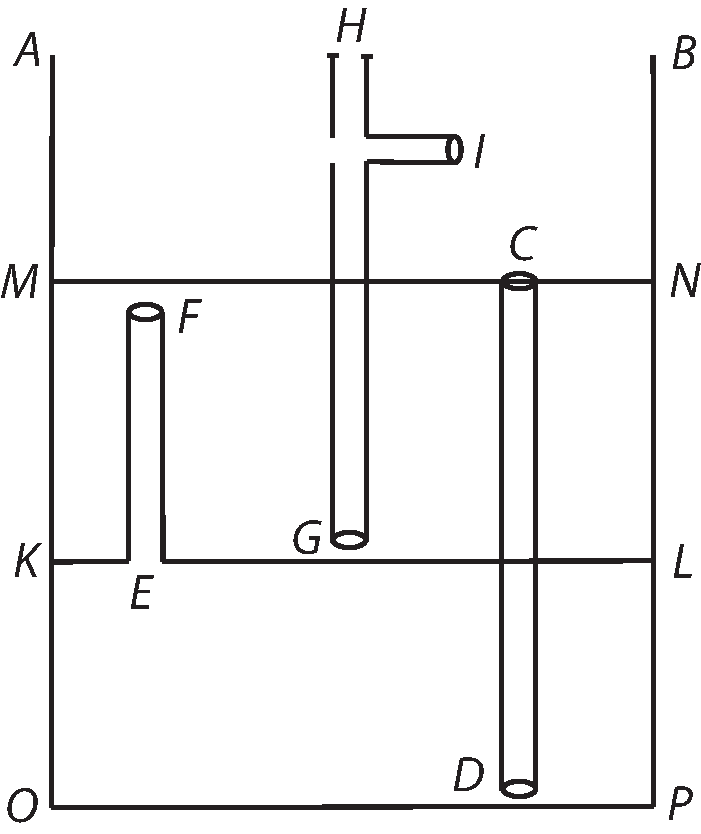
\includegraphics[trim = 0mm -2mm -5mm 0mm, clip, width=0.41\textwidth]{images/LH035,14,02_155r-d.pdf}
%\noindent \centering [\textit{Fig. 1}]
%\end{wrapfigure}
\textit{Si comprimatur aer in vase pneumatico, cujus inferiorem partem aqua occupet,} (+~puto superiorem +) 
\textit{inde cum tanto impetu aqua erumpet, ut quamlibet fere datam altitudinem per se superare possit, quod ut in simplici organo intelligas sit vas pneumaticum initio propositum \textso{KP} cujus portio inferior \textso{QP} aquam contineatur, superior \textso{QI} aera, jam}
\noindent
\textit{per tubum intrusus saepius repetitis scilicet vicibus aer more solito comprimatur in} \makebox[1.0\textwidth][s]{\textit{cavitate}
\textit{\textso{KR}}\textit{. tum probe occludatur tubus} (quo aer intrat)
\textit{\textso{FM},}
\textit{advoluta scilicet clavicula}}
\pend
\newpage
\pstart
\centering
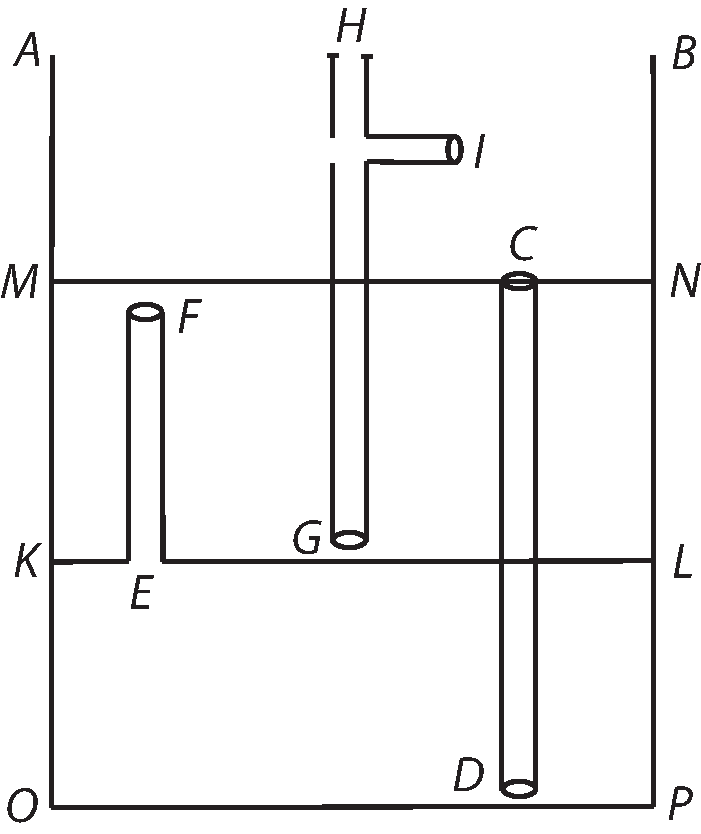
\includegraphics[trim = 0mm 0mm 0mm 0mm, clip, width=0.38\textwidth]{images/LH035,14,02_155r-d.pdf}\\
\noindent \centering [\textit{Fig. 1}]
\pend
\count\Bfootins=1200
\count\Cfootins=1200
\vspace{1em}
\pstart \noindent (Epistomio \setline{1}\textit{\textso{H}}.)
\textit{hoc posito si revolvatur clavicula }\textit{\textso{V},}
\textit{canaliculi} sursum ex aqua educit \textit{\textso{TS}.}\textit{ erumpet aqua per hunc eundem canaliculum ab aere compresso extrusa cum maximo impetu,} quanto major compressio. Hoc artificium jam fere commune est \textit{partim pneumaticum, partim \edtext{hydraulicum.}{\lemma{hydraulicum.}\Cfootnote{a.a.O.\cite{00044}, S. 146f.}}} \textit{Sunt multi alii modi de quibus in hydraulicis, communis ille est, qui vulgo Cardani\protect\index{Namensregister}{\textso{Cardano} (Cardanus), Girolamo (Geronimo) 1501-1576}
dicitur \edtext{quo}{\lemma{quo}\Cfootnote{a.a.O.\cite{00044}, S.~147
mit Auslassung: \textit{dicitur} [...] \textit{quo}.}}
scil. aer ab aquae pondere
\edtext{comprimitur. Sit vas quod\-libet aeneum \textso{ABPO}}{\lemma{comprimitur.}\Bfootnote{\textit{(1)}\ \textit{Sit vas} \textit{(2)}\ \textit{Sit vas pneumaticum \textso{KP}, cujus portio inferior \textso{QP}} \textit{(3)}\ \textit{Sit vas quodlibet aeneum \textso{ABPO}} \textit{L}}}}
%keine zweite Zeichnung auf Handschrift
\textit{in tres regiones separatas distinctum, scilicet in infimam }\textit{\textso{OL}}\textit{ mediam }\textit{\textso{KN}}\textit{ et supremam }\textit{\textso{MB}}\textit{ apertam atque patentem, sint tres canaliculi primus major }\textit{\textso{CD}}\textit{ cujus altera extremitas }\textit{\textso{D}}\textit{ ad basin }\textit{\textso{OP}}\textit{ tantum non pertingat, sed modica pateat rima in infimam regionem }\textit{\textso{OL}}\textit{, secundus }\textit{\textso{EF}}\textit{ ab infima regione ad mediam ita ductus, ut ad }\textit{\textso{MN}}\textit{ mediae tantum non perveniat, ultimus denique omnium minimus \textso{GH} ab imo mediae regionis ad supremam paulo liberius extans, cum clavicula}
\textit{\textso{I}}\textit{ hoc supposito, per canaliculum }\textit{\textso{HG}}\textit{ immittatur aqua in mediam regionem }\textit{\textso{KN}}\textit{, ita tamen ut} usque ad \textit{\textso{F}} non pertingat, ne scilicet per \edtext{[canaliculum]}{\lemma{canalicum}\Bfootnote{\textit{L ändert Hrsg. nach Vorlage}}} \textit{\textso{EF}} in infimam regionem influat, \textit{tum advoluta clavicula }\textit{\textso{I}}\textit{, probe obstruatur} \edtext{[\textit{canaliculus}]}{\lemma{\textit{caniculus}}\Bfootnote{\textit{L ändert Hrsg. nach Vorlage}}}
\textit{\textso{GH}}\textit{ deinde tota cavitas suprema }\textit{\textso{AN}}\textit{ aqua impleatur, et mox aperiatur foramen} \textit{\textso{C,}} \textit{hinc enim fiet, ut aqua suo pondere aera contentum in infima regione }\textit{\textso{OL}}\textit{ comprimat, qui cum per canaliculum }\textit{\textso{DC}}\textit{ regredi non possit, quia statim aqua occludit rimam infimam }\textit{\textso{D}}\textit{ et multum aquae inferiorem tractum regionis \textso{OL} occupat, comprimitur in superiorem tractum, idque tamdiu, quamdiu pondus aquae praevalet seu superat aeris resistentiam, tamdiu enim aqua per canalem \textso{CD} in \textso{OL} subit,} \edtext{[\textit{at}]}{\lemma{}\Bfootnote{\textit{ad}\textit{\ L \"{a}ndert Hrsg. nach Vorlage}}}
\textit{ubi perventum est ad aequalitatem ponderis et resistentiae, aperiatur canaliculus \textso{GH}, revoluta scilicet
clavicula \textso{I} aerque compressus per \textso{EF} vim suam imprimet summae superficiei aquae, contentae intra
mediam regionem \textso{ML}, eamque per foramen G
et angustiorem canaliculum \textso{GH} foras extrudet, ludusque
tamdiu durabit quamdiu aer ab aqua per
majorem canalem \textso{CD} subeunte comprimetur,
at ubi semel aqua totam regionem \textso{OL} occuparit, non amplius ullum aera comprimere \edtext{potest.}{\lemma{potest}\Cfootnote{a.a.O.\cite{00044}, S. 147.}}}
[156~r\textsuperscript{o}]
\pend%
\count\Bfootins=1000
\count\Cfootins=1000
\pstart%
%
%
%
% \input{gesamttex/edit/LH035_14_02_156r.tex}
% [156~r\textsuperscript{o}]
\textso{Honor. Fab. Tract.} \pgrk{F}\,\textso{ys. 1. lib. 2. prop. 265.} Si qua recta extensa ad instar fili continuo ab uno puncto versus alterum tentescere cogitetur, si aequaliter resultat arcus circuli, si juxta quadrata distantiarum ab extremo uno resultat parabola, si inaequaliter sed juxta rationem distantiarum, resultavit curva quaedam nova hactenus innominata. Parabola est v.g. si vis tensionis distribuitur singulis non tantum ratione distantiae\protect\index{Sachverzeichnis}{ratio distantiae} sed etiam ratione ponderis\protect\index{Sachverzeichnis}{ratio ponderis}, fitque ratio composita ponderum et \edtext{distantiarum.}{\lemma{distantiarum.}\Cfootnote{a.a.O.\cite{00044}, S. 168-170.}}
\textit{At si in singulis punctis consideretur idem pondus, distantia tantum diversa, incurvatio fit in dictam \edtext{curvam.}{\lemma{curvam.}\Cfootnote{a.a.O.\cite{00044}, S. 170.}}}
\textit{Si cylinder vel parallelepipedum vel prisma parieti \edtext{affigatur,}{\lemma{affigatur,}\Cfootnote{a.a.O.\cite{00044}, S. 170.}}} proprio pondere in parabolam incurvatur. Primusque hanc cogitationem Galilaeus\protect\index{Namensregister}{\textso{Galilei} (Galilaeus, Galileus), Galileo 1564-1642} menti injecit, qui quanquam sine demonstratione dixit, \textit{funem utrinque alligatum in \edtext{parabolam}{\lemma{parabolam}\Cfootnote{\textsc{G. Galilei}, \title{Discorsi}\cite{00050}, Leiden 1638, S. 146 (\title{GO}\cite{00048} VIII, S. 185f.)}}} \edtext{[\textit{incurvari}].}{{\lemma{\textit{alligari}}\Bfootnote{\textit{L \"{a}ndert Hrsg. nach Vorlage}}}{\lemma{[\textit{incurvari}]}\Cfootnote{\textsc{H. Fabri}, \title{Physica}\cite{00044}, Bd. 1, Lyon 1669, S. 170.}}}
\pend
\pstart \textso{Honor. Fab. Tract.} \pgrk{F}\,\textso{ys. 1. lib. 2. prop. 298.} Quando et arcus et chorda\protect\index{Sachverzeichnis}{arcus et chorda}, tunc ratio tensionis componi debet.
\textit{Posita duorum arcuum ejusdem longitudinis sed diversae structurae aequalitate virium nisus initio reductionis majorem vim \edtext{acquirit,}{\lemma{acquirit,}\Cfootnote{a.a.O.\cite{00044}, S. 186.}}} cujus extremitates majus spatium percurrunt.
\textit{Hinc ut magis adducantur per tensionem, extremitates arcus\protect\index{Sachverzeichnis}{extremitates arcus} maxime imminuitur corpus arcus versus easdem extremitates scil. vel in conum, vel in pyramidem, vel in solidum quod nascitur ex sectione parallelepipedi vel cylindri per diagonalem, vel ex solido parabolico, sive convexo sive concavo, haec ultima ratio solidi maxime confert ad maximam adductionem positis iisdem viribus \edtext{adducentibus}{\lemma{adducentibus}\Cfootnote{a.a.O.\cite{00044}, S. 186.}}} idem confert ratio solidi conici vel \edtext{pyramidalis.}{\lemma{pyramidalis.}\Cfootnote{a.a.O.\cite{00044}, S. 186.}}
\pend
\newpage
\pstart
%
\centering 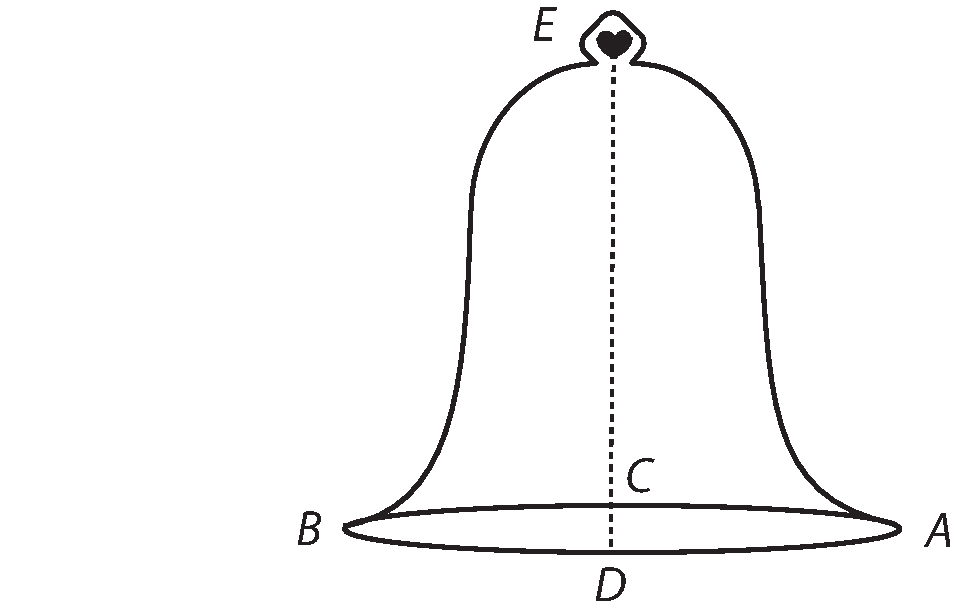
\includegraphics[trim = 0mm 0mm 0mm 0mm, clip, width=0.37\textwidth]{images/LH035,14,02_156r-d.pdf}\\
\noindent \centering [\textit{Fig. 2}]
\pend
\vspace{1em}
\count\Bfootins=1200
\count\Cfootins=1200
\pstart
Hinc \setline{1}in tudiculis (+ Keilen, clava +) manubrium versus extremitatem minuitur. Porro ad tensionis 
restitutionem\protect\index{Sachverzeichnis}{restitutio tensionis} retardandam cochlea\protect\index{Sachverzeichnis}{cochlea} adhiberi potest in qua zona spiralis tendatur, et \textit{in ea proportione magis tendetur in qua magis \edtext{incurvabitur,}{\lemma{incurvabitur,}\Cfootnote{a.a.O.\cite{00044}, S. 187.}} hanc spiralem zonam tensam adhibent artifices ad conciliandum motum denticulatis horologiolis, quarum jam usus communis \edtext{est.}{\lemma{est.}\Cfootnote{a.a.O.\cite{00044}, S. 187.}}} Huc revoca laminas\protect\index{Sachverzeichnis}{laminae ferreae}
\textit{ferreas quarum tensio vim facit vel in catapultis rotatis\protect\index{Sachverzeichnis}{catapulta rotata}, vel in seris, vel in quolibet alio organo, quod opera elateris \edtext{movetur.}{\lemma{movetur.}\Cfootnote{a.a.O.\cite{00044}, S. 187.}}}
\textit{Vis impressa sagittae\protect\index{Sachverzeichnis}{vis sagittae} est ut tota vis \edtext{nisus}{\lemma{nisus}\Cfootnote{a.a.O.\cite{00044}, S. 188.}}} nec refert sagittam in ultimo momento restitutionis tangas, an aliquandiu secum ferat Tensiones a posteriori optime noscuntur ope sonorum, nam
\textit{soni sunt ut tempora vibrationum\protect\index{Sachverzeichnis}{tempora vibrationum}, et haec in ratione subduplicata \edtext{spatiorum.}{\lemma{spatiorum.}\Cfootnote{a.a.O.\cite{00044}, S. 188.}}} Pulsatae campanae\protect\index{Sachverzeichnis}{campanae pulsatae} eundem sonum edunt, sive pulsentur a malleo in cava superficie sive in convexa, imo si a duplici malleo pulsentur \edtext{in punctis oppositis}{\lemma{}\Bfootnote{in punctis oppositis \textit{erg.} \textit{L}}} majorem edunt sonum quia major \edtext{tensio.}{\lemma{tensio.}\Cfootnote{a.a.O.\cite{00044}, S. 188.}} Interim nota \textit{esse quasi geminum axem in campana tensa\protect\index{Sachverzeichnis}{campana tensa}: 
Sit enim campana \textso{EBA}
si pulsetur in B vides circulum \textso{BCDA} tendi in ellipsin, itemque \textso{BEA} tendi \edtext{circa E.}{\lemma{circa E.}\Cfootnote{a.a.O.\cite{00044}, S. 189.}}} \edlabel{LH035_14_02_138-158_1a}Huc revoca scyphum\protect\index{Sachverzeichnis}{scyphus} in vitreum,
\textit{cujus si supremus limbus\protect\index{Sachverzeichnis}{limbus supremus} madenti digito affricetur, sonum edit, qui scilicet oritur ex vibrationibus, quas tum oculo tum manu probare poteris, imo quae tremulum et ferventem motum aquae intra scyphum contentae \edtext{conciliat.}{\lemma{conciliat.}\Cfootnote{a.a.O.\cite{00044}, S. 189.}}}
\pend
\count\Bfootins=1200
\count\Cfootins=1200
\pstart
\textso{Hon. Fab. Tract.} \pgrk{F}\,\textso{ys. 1. lib. 3. prop. 35.} Innumeri sunt rarefactionis\protect\index{Sachverzeichnis}{rarefactio} et condensationis\protect\index{Sachverzeichnis}{condensatio} effectus. Inter alia hi potissimi. Calor corpora reddit rariora, et \edtext{ideo leviora}{\lemma{ideo}\Bfootnote{\textit{(1)}\ graviora \textit{(2)}\ leviora, \textit{L}}}, frigus\protect\index{Sachverzeichnis}{frigus} densiora igitur graviora; unde corpora rara avolant ut halitus\protect\index{Sachverzeichnis}{halitus}, densata descendunt, ut ros, pluvia grando. Calor corpora rarefacit. Rarefactionem sequitur resolutio\protect\index{Sachverzeichnis}{resolutio}, hanc homogeneorum collectio\protect\index{Sachverzeichnis}{collectio homogeneorum} contra frigus densat, hinc collectio heterogeneorum\protect\index{Sachverzeichnis}{collectio heterogeneorum}.
\textit{Aqua quae rarescit facile sursum \edtext{avolat,}{\lemma{avolat,}\Cfootnote{a.a.O.\cite{00044}, S. 225.}} et per medium corporum \edtext{plexum, cum ipsa sit}{\lemma{plexum,}\Bfootnote{\textit{(1)}\ id est \textit{(2)}\ \textit{cum ipsa sit} \textit{L}}} humida, corpora autem habeant plexum a quibusdam filaminibus; id est igne seu materia pingui\protect\index{Sachverzeichnis}{materia pingui}. Ita succus pinguior difficilius avolat hinc pinguior jusculi portio in olla manet, hinc calore facilius siccatur pannus aqua quam oleo imbutus. Bullae quae in superficie ferventis aquae intumescunt sunt ab exteriore et quasi supernatante}
\edtext{[\textit{uligine}]}{\lemma{origine}\Bfootnote{\textit{L ändert Hrsg. nach Vorlage}}}\textit{,
quam vapor \edtext{inclusus,}{\lemma{inclusus,}\Cfootnote{a.a.O.\cite{00044}, S. 225.}}} h.e. aqua rarefacta\protect\index{Sachverzeichnis}{aqua rarefacta} inflat. Hinc pinguiora et tenaciora, lac\protect\index{Sachverzeichnis}{lac} mel butyrum\protect\index{Sachverzeichnis}{butyrum}, dum rarescunt maxime inflantur.
\textit{Quae concrescunt per densitatem albescunt, saltem ex aliqua parte, uti oleum\protect\index{Sachverzeichnis}{oleum}, butyrum, adeps \edtext{etc.}{\lemma{etc.}\Cfootnote{a.a.O.\cite{00044}, S. 225.}} quia cum aequaliter particulae condensentur, aequaliter contrahuntur, igitur in orbem, atqui in orbem concreta constant ex \edtext{sphaerulis,}{\lemma{sphaerulis,}\Cfootnote{a.a.O.\cite{00044}, S. 225.}} ut patet in spuma nive\protect\index{Sachverzeichnis}{spuma nive}, hinc albedo, denique a raritate et densitate, omnis res tormentaria et ei cognata in meteorologica\protect\index{Sachverzeichnis}{meteorologica} Mixtorum compositio, resolutio, concretio plantarum\protect\index{Sachverzeichnis}{concretio plantarum}, animalium\protect\index{Sachverzeichnis}{concretio animalium}, nutritio, formatio, augmentum; terrae motus, coctio destillatio \edtext{etc.}{\lemma{etc.}\Cfootnote{a.a.O.\cite{00044}, S. 226.}}}\edlabel{LH035_14_02_138-158_1b}
% \edtext{}{{\xxref{LH035_14_02_138-158_1a}{LH035_14_02_138-158_1b}}\lemma{}\Afootnote{\textit{Am Rand auf gleicher Höhe gegenläufig nicht von Leibniz' Hand:} C. Seriatim. 14.}}
[157~v\textsuperscript{o}]
\pend%
\pstart%
%
%
%
% \input{gesamttex/edit/LH035_14_02_157v.tex}
% [157~v\textsuperscript{o}]
\textso{Honor. Fab. tract.} \pgrk{F}\,\textso{ysic. 1. lib. 4. prop. 48.} Motus per perpendicularem ad motum per inclinatam\protect\index{Sachverzeichnis}{motus per inclinatam} in eandem basin, est ut inclinata ad perpendicularem. Et ita fit \edtext{permutatio.}{\lemma{permutatio.}\Cfootnote{a.a.O.\cite{00044}, S. 260.}}
\pend 
\pstart
\textso{Honor. Fab. tract.} \pgrk{F}\,\textso{ysic. 1. lib. 4. prop. 53.} Causa \edtext{diversitatis gravitatis et levitatis est raritas et}{\lemma{diversitatis}\Bfootnote{\textit{(1)}\ raritatis et densitatis est \textit{(a)}\ gra \textit{(b)}\ rari \textit{(2)}\ gravitatis [...] densitas. \textit{L}}} \edtext{densitas}{\lemma{densitas.}\Cfootnote{a.a.O.\cite{00044}, S. 261.}}.
\pend 
\pstart
\textso{Honor. Fab. tract.} \pgrk{F}\,\textso{ysic. 1. lib. 4. prop. 58.} Libra plumae et plumbi sunt ejusdem ponderis, non tamen ejusdem gravitatis, requirit \edtext{enim gravitatis comparatio aequalitatem}{\lemma{enim}\Bfootnote{\textit{(1)}\ plumbum diversam \textit{(2)}\ gravitatis comparatio aequalitatem extensionis. \textit{L}}} \edtext{extensionis.}{\lemma{extensionis.}\Cfootnote{a.a.O.\cite{00044}, S. 263.}}
\pend
\pstart
\textso{Honor. Fab. tract.} \pgrk{F}\,\textso{ysic. 1. lib. 4. prop. 62.}
\textit{Corpus leve non fertur sursum a principio \edtext{\textit{intrinseco,}}{\lemma{intrinseco,}\Cfootnote{a.a.O.\cite{00044}, S. 264.}}} rectissime. Gravitas per naturam intendit ad constituendum globum, levitas absoluta\protect\index{Sachverzeichnis}{levitas absoluta} dissolveret globum (+ NB. talis esset levitas absoluta
\edtext{in sole}{\lemma{}\Bfootnote{in \textbar\ radiis \textit{gestr.}\ \textbar\ sole \textit{L}}} perpetuo extrorsum agente. +) Rationes habet egregias, quia si \textit{sit vas 40 libras aquae continens,} et \textit{sit lignum immersum pendens 10 \edtext{\textit{libras,}}{\lemma{libras,}\Cfootnote{a.a.O.\cite{00044}, S. 266.}}} si aquam et lignum simul etiam dum acsendere \textit{nititur appendas, 50 libras \edtext{invenies.}{\lemma{invenies.}\Cfootnote{a.a.O.\cite{00044}, S. 266.}}} (+ NB. at aliud forte, si res insit quae Elatere sursum tendat, ut res arcu explosa, piscis, ut Schwenterus\protect\index{Namensregister}{\textso{Schwenter}, Daniel 1585-1636} ait NB. +) \textit{Si vas aqua plenum perfodiatur ad basin seu fundum et acus levissima lignea v.g. immergatur in cylindrum aquae foramini respondentem, nullo modo emergit quia scil. ab aqua deorsum fluente non extruditur vel exploditur, atqui revera emergeret, si ab intrinseco sursum \edtext{ascenderet.}{\lemma{ascenderet.}\Cfootnote{a.a.O.\cite{00044}, S. 266.}}} (+ NB. notabile experimentum hydrostaticum\protect\index{Sachverzeichnis}{experimentum hydrostaticum}. +)
\textit{Deinde quando ventus per lineam horizontalem paulo vehementius flat, nihil fumi ex camino erumpit} (+~NB~+)
\textit{quia scilicet aer non descendit a vento actus, igitur ideo fumus ascendit quia ab aere
extruditur. Aer
rarior ab aestu non ita fumum extrudit quia} tunc \textit{levior \edtext{est}{\lemma{est}\Cfootnote{a.a.O.\cite{00044}, S. 266.}}}; et sane haec de fumo tractatio multum ad rem pertinet. Ergo fumus\protect\index{Sachverzeichnis}{fumus} non propria levitate surgit si virgula lignea immersa extruditur, quo plus est aquae fortius extruditur non deberet si propria vi surgeret.
Aristotelis\protect\index{Namensregister}{\textso{Aristoteles}, 384-322 v. Chr.} autoritas\protect\index{Sachverzeichnis}{Aristotelis autoritas} contraria hic non est curanda. Nam idem quoque statuit \textit{ex duobus corporibus \edtext{inaequalibus ejusdem materiae et figurae majus}{\lemma{inaequalibus}\Bfootnote{\textit{(1)}\ \textit{majoris} \textit{(2)}\ \textit{ejusdem materiae et figurae majus} \textit{L}}} velocius descendere: ex duobus aequalibus, sed} disquiponderantibus gravius in gravitatis ratione velocius descendere. Item grave per diversa media in ea proportione descendere, in qua est unum medium alio \edtext{densius.}{\lemma{densius.}\Cfootnote{a.a.O.\cite{00044}, S. 268.}}
\pend
\pstart \textso{Honor. Fab. tract.} \pgrk{F}\,\textso{ysic. 1. lib. 4. prop. 69.} In descensione\protect\index{Sachverzeichnis}{descensio gravium} et gravitatione gravium in aliquo medio momenta librae quasi observari possunt, accepta aequali extensione, ut in libra aequalibus distantiis. Nam si partes extrudentes in eadem extensione sunt graviores irruentibus, natat, non descendit \edtext{grave. Corpus}{\lemma{grave.}\Bfootnote{\textit{(1)}\ Unde semper pars extrudendi non extruditur; quae \textit{(2)}\ Corpus \textit{L}}} grave quadruplo densius velocius descendet quam duplo \edtext{densius.}{\lemma{densius.}\Cfootnote{a.a.O.\cite{00044}, S. 270.}}
\pend
\pstart
\textso{Honor. Fab. tract.} \pgrk{F}\,\textso{ysic. 1. lib. 4. prop. 71.} Globus plumbeus\protect\index{Sachverzeichnis}{globus plumbeus} velocius descendit quam ligneus\protect\index{Sachverzeichnis}{globus ligneus}. At si sibi \edtext{imponantur, ligneus imponatur plumbeo}{\lemma{imponantur,}\Bfootnote{\textit{(1)}\ ita at plumbeus \textit{(2)}\ ligneus imponatur plumbeo, \textit{L}}}, descendent simul quasi conferruminata. Huius rationem non reddit
Honoratus Fabri\protect\index{Namensregister}{\textso{Fabri}, Honor\'{e} SJ 1607-1688} solidam. Ego hanc affero, quia ne detur vacuum \edtext{grande}{\lemma{}\Bfootnote{grande \textit{erg.} \textit{L}}} non separantur seu cohaerent. Sed experientia quaerenda est. Videtur tamen ipse innuere negatam sibi a quibusdam descensus \edtext{inaequalitatem.}{\lemma{inaequalitatem.}\Cfootnote{a.a.O.\cite{00044}, S. 271.}}
\pend 
\newpage
\pstart 
\textso{Honor. Fab. tract.} \pgrk{F}\,\textso{ysic. 1. lib. 4. prop. 78.} Cum acuminata corpora facilius medium findant, hinc naves\protect\index{Sachverzeichnis}{navis} mucrone aquas secant, globus velocius descendit quam cubus\protect\index{Sachverzeichnis}{cubus}, cubus angulo quam plano, de proportione alibi. Duo globi \edtext{diversae materiae inaequaliter}{\lemma{diversae}\Bfootnote{\textit{(1)}\ gravitatis oe \textit{(2)}\ materiae inaequaliter descendunt. \textit{L}}} \edtext{descendunt.}{\lemma{descendunt.}\Cfootnote{a.a.O.\cite{00044}, S. 276.}}
\pend
\pstart
\textso{Honor. Fab. tract.} \pgrk{F}\,\textso{ysic. 1. lib. 4. prop. 81.} Nullius momenti est argumentum vulgare contra motum in vacuo dicunt enim fore infinite celerem seu instantaneum, id est nullum, sed hoc ait non esse necesse. Sit enim inquit in motu in vacuo ut 1. \textit{in motu in medio aeque denso ut 0. In medio duplo rariore erat ut} 
\rule[-2mm]{0mm}{8mm}$\displaystyle1-\frac{1}{2}$, 
\textit{in triplo rariore ut} 
\rule[-4mm]{0mm}{0mm}$\displaystyle1-\frac{1}{3}$
\textit{\edtext{egregie.}{\lemma{egregie.}\Cfootnote{a.a.O.\cite{00044}, S. 278.}}}
Hinc porro celeritatis gravium\protect\index{Sachverzeichnis}{celeritas gravium} inaequaliter inaequalis in mediocri altitudine nulla est differentia sensibilis. v.g. sit lapis 2000 mahl gravior aere,
lignum 500 mahl,\edtext{ detrahitur lapidi}{\lemma{detrahitur}\Bfootnote{\textit{(1)}\ aquae \textit{(2)}\ lapidi \textit{L}}} gravitatis in vacuo\protect\index{Sachverzeichnis}{gravitas in vacuo}, seu per se 
\rule[-2mm]{0mm}{8mm}$\displaystyle1-\frac{1}{2000}$
ligno $\displaystyle1-\frac{1}{500}$.
Unde in aere
lapis descendet ut 1999 lignum ut
\rule[-4mm]{0mm}{0mm}$\displaystyle1-\frac{1}{1999}$
caeterum habenda ratio non tantum gravitatis medii, sed et implexionis seu tenacitatis, qua nec aer
omnino caret, quae multum retardat, hinc corporum levissimorum in aere
tardatur \edtext{motus.}{\lemma{motus.}\Cfootnote{a.a.O.\cite{00044}, S. 278.}}
Hinc forte funependulum longissimum pauciores aestate\protect\index{Sachverzeichnis}{aestas} dato tempore conficit vibrationes\protect\index{Sachverzeichnis}{vibrationes}, quam hyeme\protect\index{Sachverzeichnis}{hyems}. Quod crebriora tunc halituum a calore filamina. Ergo male quidam, si verum est, referunt in motum \edtext{terrae.}{\lemma{terrae.}\Cfootnote{a.a.O.\cite{00044}, S. 279.}}
\pend 
\pstart
\textso{Honor. Fab. tract.} \pgrk{F}\,\textso{ysic. 1. lib. 4. prop. 84.}
\textit{Si aqua in Vase perforato contineatur et lamina lignea levissima vel palea respondeat foramini vel sit intra cylindrum aquae\protect\index{Sachverzeichnis}{cylinder aquae} cujus foramen est basis nullo modo sursum \textit{extruditur. \edtext{Hinc}{\lemma{\textit{Hinc.}}\Cfootnote{a.a.O.\cite{00044}, S. 279 mit Auslassung: \textit{extruditur.} [...] \textit{Hinc.}}}}
%
\textit{si
quando occurrant aquarum voragines levissima etiam corpora absorbentur. Hinc si lagenam aqua plenam\protect\index{Sachverzeichnis}{lagena plena} invertas levissima etiam corpora cum aqua per lagenae collum} 
\edtext{\textit{descendunt.}}{\lemma{\textit{descendunt.}}\Cfootnote{a.a.O.\cite{00044}, S. 279 mit Auslassung: \textit{absorbentur.} [...] \textit{Hinc}.}}} 
Haec ratio et in vorticibus fluminum
\textit{ii autem in gyros eunt, quia cum recta intrare non possit ob aerem explodendum circulo \edtext{constat exemplum}{\lemma{constat}\Bfootnote{\textit{(1)}\ qua \textit{(2)}\ \textit{exemplum} \textit{L}}} habemus et in calamo \edtext{volatili.}{\lemma{volatili.}\Cfootnote{a.a.O.\cite{00044}, S.~279.}}}
[150~v\textsuperscript{o}]
\pend %
%\newpage
\pstart%
% O. nam. 5.\edtext{}{\lemma{5.}\Cfootnote{Nicht von Leibniz' Hand, gegenl\"{a}ufig am rechten unteren Rand.}}
%
%
%
% \input{gesamttex/edit/LH035_14_02_150v.tex}
% [150~v\textsuperscript{o}]
\textso{Honorat. Fab. Tract. 1.} \pgrk{F}\,\textso{ys. lib. 4. prop. 85.}
\textit{Virgula\protect\index{Sachverzeichnis}{virgula} in situ verticali aquae immersa, eo majore vi extruditur quo altior est \edtext{aqua.}{\lemma{aqua.}\Cfootnote{a.a.O.\cite{00044}, S. 279f.}}} (+ Hic errare videtur, et ratio eius est nullius momenti. +)
\textso{Honorat. Fab. Tract. 1.} \pgrk{F}\,\textso{ys. lib. 4. prop. 86. sqq.}
\textit{Si sit tubus perpendiculariter erectus juxta basin ad latus perforatus, primumque aqua plenus majore vi aqua per foramen extruditur, quando tubus altior \edtext{est.}{\lemma{est.}\Cfootnote{a.a.O.\cite{00044}, S. 280.}}} Unde si juxta basin conchae aquae ductus componatur longe plus aquae exuget, quam si juxta superiorem marginem admoveretur. \textit{Motus sunt in ratione subduplicata\protect\index{Sachverzeichnis}{ratio subduplicata} virium} \edtext{extrudentium}{\lemma{extrudentium}\Cfootnote{a.a.O.\cite{00044}, S. 280.}}, seu \edtext{\textit{vires sunt ut}
[\textit{quadrata;}]}{\lemma{radices}\Bfootnote{\textit{L ändert Hrsg. nach Vorlage}}}
\textit{motus ut}
\edtext{[\textit{radices}].}{{\lemma{quadrata}\Bfootnote{\textit{L ändert Hrsg. nach Vorlage}}}%
{\lemma{[\textit{radices}]}\Cfootnote{a.a.O.\cite{00044}, S.~281.}}}
Quia vires tantae quantus effectus.
\edtext{Effectus quantitas sumenda non tantum}{\lemma{Effectus}\Bfootnote{\textit{(1)}\ tantus \textit{(2)} quantitas sumenda non tantum \textit{L}}} a celeri motu sed et quantitate materiae extrusae, ut si duplo celeriore motu tantundem extrudatur vires erunt duplae, si duplo celeriore motu duplum extrudatur erunt quadruplae. Haec jam obtinent sive aqua proprio pondere, sive ab alio extrudatur.
\pend
\pstart
\textit{Aqua per foramen Tubi extrusa eam habet impetus\protect\index{Sachverzeichnis}{impetus aqjae} vim seu velocitatis\protect\index{Sachverzeichnis}{velocitas aquae} gradum, quem acquisivisset si ex summo
\edtext{tubo,}{\lemma{tubo,}\Cfootnote{a.a.O.\cite{00044}, S. 283.}}} seu superficie aquae delapsa fuisset. Haec est propositio
Torricellii\protect\index{Namensregister}{\textso{Torricelli}, Evangelista 1608-1647} lib. 2. de motu \edtext{projectorum,}{\lemma{projectorum,}\Cfootnote{\textsc{E. Torricelli}, \title{De motu gravium}\cite{00304}, Florenz 1644, S.~191f.}} ex qua plerasque omnes quas ibi de motu aquae\protect\index{Sachverzeichnis}{motus aquae} habet deduci, et tamen eam tantum verisimiliter confirmat. Ex nostris principiis demonstratur statim, quia motus sunt in subduplicata altitudinum ratione\protect\index{Sachverzeichnis}{ratio subduplicata}.
\textit{Dices hoc repugnare experimento sit enim tubus \textso{AC} cum canali \textso{CD} aperto sursum in \textso{D} si tubo aqua pleno} 
\pend
\vspace{1em}
\pstart
\centering
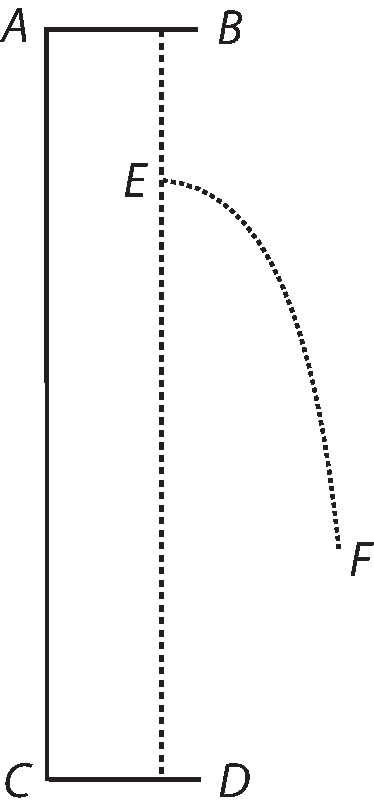
\includegraphics[trim = 0mm 0mm 0mm 0mm, clip, width=0.21\textwidth]{images/LH035,14,02_150v-d1.pdf}\\
\noindent \centering [\textit{Fig. 3}]
\pend
\count\Bfootins=1300
\count\Cfootins=1300
\newpage
\pstart \noindent \textit{aperiatur foramen \textso{D} erumpit quidem aqua sursum per lineam \textso{DE} caditque per \textso{EF} nunquam tamen ad libellam \textso{AB}
\edtext{sed}{\lemma{sed}\Cfootnote{\textsc{H. Fabri}, \title{Physica}\cite{00044}, Bd. 1, Lyon 1669, S. 283.}}} recte respondet \textit{Torricellius\protect\index{Namensregister}{\textso{Torricelli}, Evangelista 1608-1647} impediri cum ab aere dispergente, tum maxime quia superiores guttae ut deinde descendant, motum aliarum subsequentium suo pondere deprimunt et tardant. Hinc si uno et primo impetu aperto primum foramine }\textit{\textso{D}}\textit{ aqua erumpat, altius haud dubie \edtext{ascendet,}{\lemma{ascendet,}\Cfootnote{a.a.O.\cite{00044}, S. 283.}} porro aqua per foramen extrusa describit eandem lineam quam projectum per \edtext{horizontalem.}{\lemma{horizontalem.}\Cfootnote{a.a.O.\cite{00044}, S. 284.}}} Id est parabolam etsi experimento non appareat ob aerem despergentem. Porro \textit{si per siphonem solito more aqua extrigatur quantitates aquae exugentis sunt in subduplicata ratione altitudinum \edtext{siphonum.}{\lemma{siphonum.}\Cfootnote{a.a.O.\cite{00044}, S. 285.}}}
\pend
\pstart
\textso{Prop. }\edtext{[\textso{102.}]}{\lemma{}\Bfootnote{\textso{202.}\textit{\ L \"{a}ndert Hrsg. }}} Ratio \textit{circulorum\protect\index{Sachverzeichnis}{ratio circulorum} qui se circa idem centrum explicant,} dum aliquid \textit{immergitur, quia scilicet aquae quae sensim et quasi per superficies attollitur, cum extare non possit, sese ad libellam \edtext{componit.}{\lemma{componit.}\Cfootnote{a.a.O.\cite{00044}, S. 288.}}}
\pend 
\count\Bfootins=1200
\count\Cfootins=1200
\pstart 
\textso{Honorat. Fab. Tract. 1.} \pgrk{F}\,\textso{ys. lib. 4. prop. 104.} 
\textit{Libra aquae potest aequipondium facere cum pluribus libris ferri, etiamsi appendantur hae in brachiis librae aequalibus. Hoc est vulgare satis experimentum.
\edtext{Sit}{\lemma{Sit}\Cfootnote{a.a.O., S.~289
mit Auslassung: \textit{experimentum.} [...] \textit{Sit}.}}
cylinder \textso{FIKG} affixus}
\textit{immobiliter muro \textso{H}, ita compositus cum alio cavo \textso{ADCB}, ut inter utrumque tantulum spatii relinquatur, sitque affixus brachio \textso{OLN} in \textso{O} sustineatur libra in \textso{M} et appendatur gravissimum pondus \textso{P} in \textso{N} statim demittitur brachium \textso{LN} et attollitur \textso{LO}, ita ut basis \textso{CD} tangat basin \textso{IK} si autem per \textso{AF} vel \textso{GB} infundas aquam donec impleat illud intermedium spatium deprimitur basis \textso{DC} nec tangit amplius basin \textso{IK} igitur tantulum aquae praevalet maximo ponderi \textso{P}.} 
Res certa est ratio difficilis,
\textit{et vix quod sciam bene explicata. Dicunt aliqui ita se habere pondus}
\textit{\textso{P}}
\textit{attollens basin}
\textit{\textso{DC}}
\textit{mobilem, et affigens immobili}
\textit{\textso{IK}}\textit{ ac si basi}
\textit{\textso{DC}}\textit{ immobili affigeret basin}
\textit{\textso{IK}}
\textit{mobilem pondus}
\textit{\textso{P}}\textit{ positum in cylindro vacuo}
\textit{\textso{FIKG}}\textit{ qui nobis navem humido innatantem repraesentat, igitur sit vas}
\textit{\textso{AC}}\textit{ cylindricum aqua plenum, immobile sit aliud cavum}
\textit{\textso{FK}}\textit{ ad instar navis; cum suo pondere}
\textit{\textso{P}}
\textit{imponatur superficiei aquae haud dubie deorsum immergitur, aqua scil. ex parte extrusa, usque ad eam altitudinem quae ponderi innatanti at aquae extrusae proportionata est, h.e. eodem modo immergitur quo immergeretur in lacum vel in fluvium, manetque in eo statu innatantis, in quo revera maneret si aquam non extrusisset, sed ab ea fuisset ex parte 
extrusus, sed hoc dici non potest quia corpus innatans, si minus suo sustineat extrusae aquae pondus, aliam adhuc ulterius extrudit; ut dictum est supra: igitur ut deorsum non immergatur, debet aquae pondus sustinere suo prorsus aequale, quod revera in hoc casu non accidit. Igitur aliunde ratio petenda est, h.e. ex aere intercepto, qui cum extrudi non possit, externae basi cylindri innatantis adhaeret: igitur videtur esse aequipondium. Quod autem ille aer extrudi non possit ratio haec est, quia cum tantum extrudatur quasi per medium cylindrum, aqua scil. in orbem ab omni parte premente, et extrudente, et cylindrus cavus innatans illam regionem occupet, per quam aer ille extrudi posset, non est mirum, si in iis angustiis detineatur ac proinde efficiat, ut praedictus cylindrus cavus innatare videatur, rem facile probabis in gemino scypho, quorum alter alteri \edtext{inseratur.}{\lemma{inseratur.}\Cfootnote{a.a.O.\cite{00044}, S. 289f.}}}
(+ non satis haec capio 1. quae aliorum sententia, 2. quomodo in sententia Honorati\protect\index{Namensregister}{\textso{Fabri}, Honor\'{e} SJ 1607-1688}
non posset exire aer, 3. quomodo inclusus aer sit causa tantae gravitatis. 4. Debeant accuratius de hac re quae magni momenti esse potest institui
\edtext{experimenta quantum debeat}{\lemma{experimenta}\Bfootnote{\textit{(1)}\ quousque \textit{(2)}\ quantum debeat \textit{L}}} maximum pondus \textit{\textso{P}}
esse ut attollatur. An non tantum augeatur pondus \textit{\textso{DC}} quantum est pondus cylindri immobilis \textit{\textso{IK}}, et multa alia experiri hic decebat. Ego putem ponderare cylindrum immobilem hac ratione mobili, quia in aquam agit, eamque extrudit seu ei resistit. Tentandum in aliis. Item tentandum si basis inferior mobilis non attingit immediate  superiorem mobilem. NB. tandem potest ope hujus rei sine dubio 
%\begin{wrapfigure}{l}{0.7\textwidth} 
%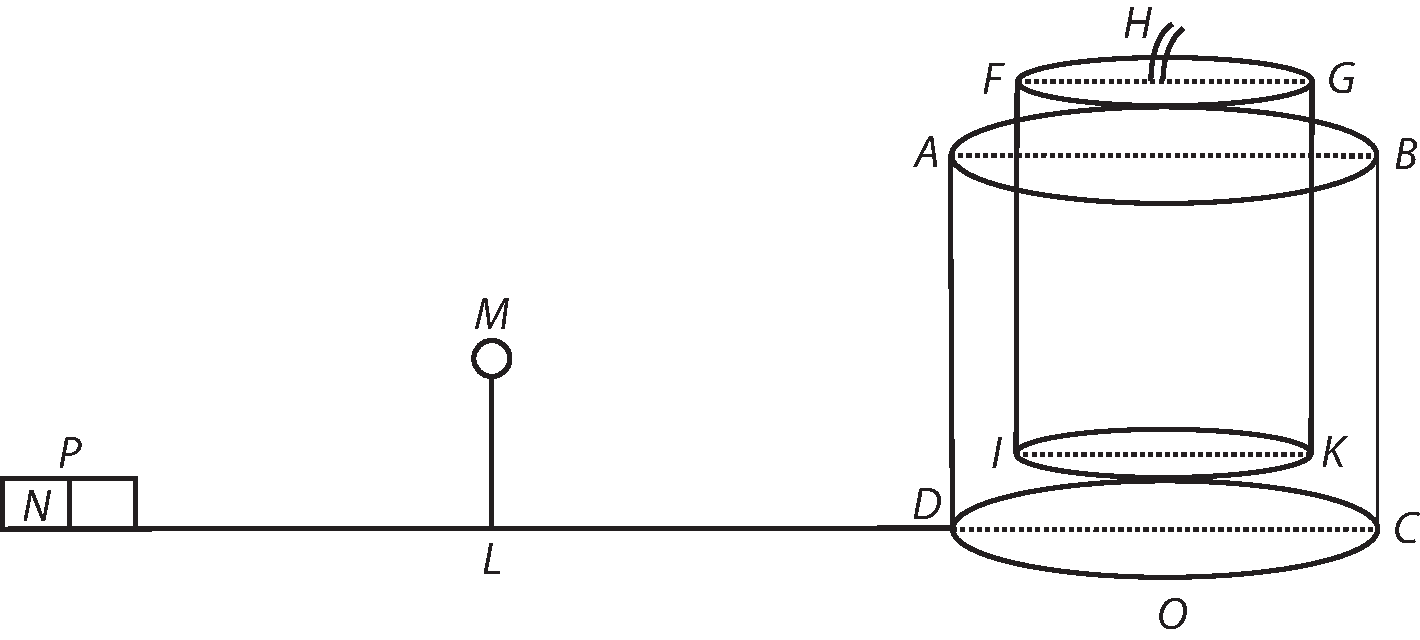
\includegraphics[width=0.7\textwidth]{images/LH035,14,02_150v-d2.pdf}\\
%\centering[\textit{Fig. 4}]
%\end{wrapfigure}
effici motus perpetuus aqua modo influente, et ita adverso pondere levato, modo ubi effluxit rursus depresso, \edtext{donec depressu suo finiat rursus influere aquam,}{\lemma{donec}\Bfootnote{\textit{(1)}\ effluxa sua rursus aq \textit{(2)}\ depressu [...] aquam, \textit{L}}} ut ascensu suo eandem iterum levabit \edtext{NB. \phantom(\hspace{-1.2mm}+)}{\lemma{NB.}\Bfootnote{\phantom(\hspace{-1.2mm}+) \textbar\ Haberi et alius motus perpertuus potest ope navis modo surgentis modo aquam subeuntis. \phantom(\hspace{-1.2mm}+) \textit{gestr.}\ \textbar\ \textit{L}}}
[149~r\textsuperscript{o}]
\pend%
\count\Bfootins=1200
\count\Cfootins=1200
\pstart%
% 
%
%
% \input{gesamttex/edit/LH035_14_02_149r.tex}
% [149~r\textsuperscript{o}]
\textso{Honorat. Fab. Tract. 1.} \pgrk{F}\,\textso{ys. lib. 4. prop. 107.}
\textit{Cum totus aer simul premat superficiem aquae attolli non potest, posita scil. aequalitate aeris quoquoversum prementis.
\edtext{Supponit}{\lemma{Supponit}\Cfootnote{a.a.O., S.~290 mit Auslassung: \textit{prementis.} [...] \textit{Supponit.}}}
haec propositio aequalem
\edtext{aeris}{\lemma{aeris}\Cfootnote{a.a.O., S.~290 mit Auslassung: \textit{aequalem} [...] \textit{aeris.}}}
altitudinem, alias
\textit{haud dubie tantulum aqua extruditur et attollitur versus illam partem, cui minor aeris portio incumbit, hinc versus terram tantulum}} \textit{attollitur aqua, hinc perpetua fluctuum atque reciproca aestuatione versus litora} \textit{mare agitatur, hinc facilius a litore naves recedunt, quam ad illud accedunt, per se.} \textit{Hinc demum\ \textso{NB.}}\ \textit{recte explicari potest ratio aestus marini, quidve ad eum Luna conferat, nempe si ea portio aeris assumatur quae inter Lunam\protect\index{Sachverzeichnis}{luna} et terram\protect\index{Sachverzeichnis}{terra} interjicitur h.e. cylindrus aeris cujus} \textit{una portio versus $\rightmoon$nam,} \textit{ut sic dicam} \textit{incumbit, seu gravitat, alia versus terram, haud dubie illa plaga terristris globi\protect\index{Sachverzeichnis}{globus terrestris}, quae hujus cylindri quasi\hfill basis\hfill est,\hfill minorem\hfill vim\hfill ab\hfill \edtext{aere\hfill gravitante\hfill\protect\index{Sachverzeichnis}{aer gravitans}}{\lemma{}\Bfootnote{\textit{aere} \textbar\ \textit{quando} \textit{gestr.}\ \textbar\ \textit{gravitante} \textit{L}}}accipit,\hfill quam\hfill aliae\hfill quibus\hfill major\hfill aeris} 
\pend 
\pstart
\centering
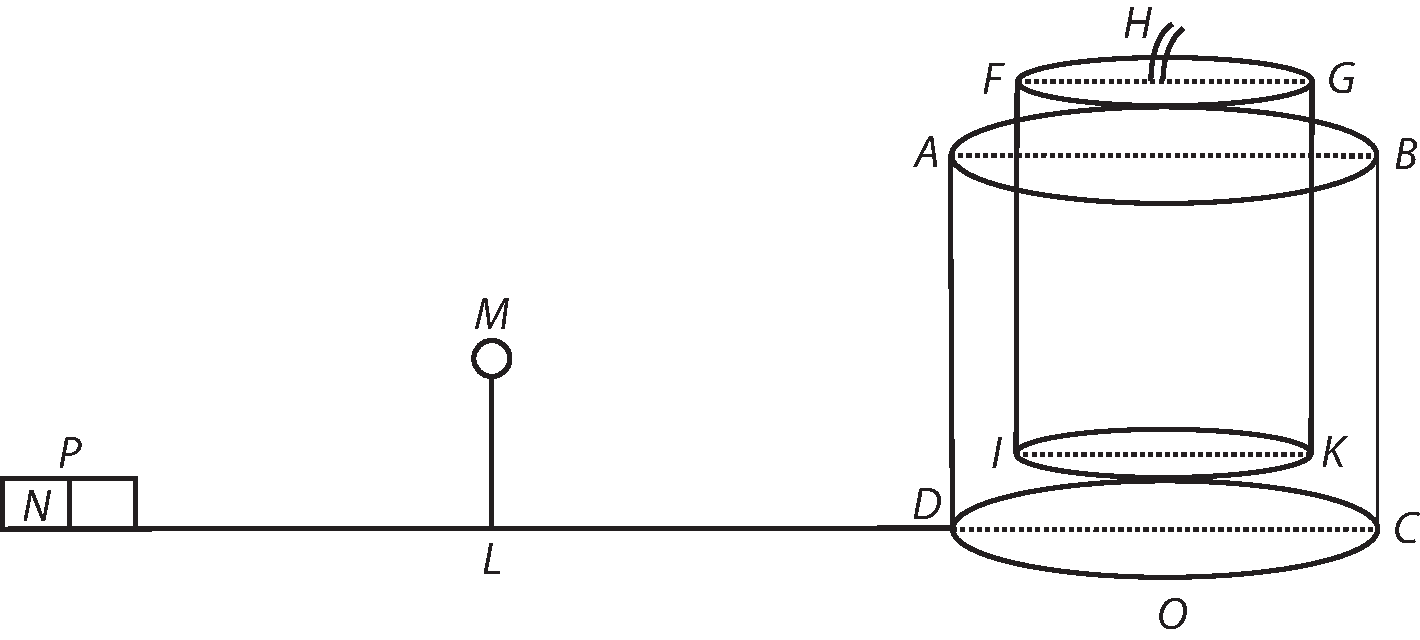
\includegraphics[width=0.84\textwidth]{images/LH035,14,02_150v-d2.pdf}\\
\centering [\textit{Fig. 4}]
\pend
\vspace{1.5em}
%\newpage
\pstart \noindent \textit{portio \setline{1}incumbit, igitur si aqua praedictam plagam occupat, necessario attolli debet, idque successive juxta lunae motum\protect\index{Sachverzeichnis}{motus lunae}, sed de} his alias
\textit{Videtur enim esse} simplex et facilis aestum marinorum explicandorum
\edtext{ratio.}{\lemma{ratio.}\Cfootnote{a.a.O.\cite{00044}, S. 290f.}}
\pend 
\count\Afootins=1200
\count\Bfootins=1100
\count\Cfootins=1100
\pstart 
\textso{Honorat. Fab. Tract. 1.} \pgrk{F}\,\textso{ys. lib. 4. prop. 114.}
\textit{Navis cujus fundi superficies
\edtext{latior}{\lemma{latior}\Cfootnote{a.a.O., S.~294
mit Auslassung: \textit{superficies} [...] \textit{latior.}}}
est non tam alte \edtext{immergitur.}{\lemma{immergitur.}\Cfootnote{a.a.O.\cite{00044}, S. 294.}}}\\
\indent
%\pend
%\pstart
\textso{Honorat. Fab. Tract. 1.} \pgrk{F}\,\textso{ys. lib. 4. prop. 116.}
\textit{Si fundus navis sit perforatus per foramen aqua sursum \edtext{erumpit}{\lemma{erumpit}\Cfootnote{a.a.O.\cite{00044}, S. 294.}}}, nam ab aqua superiore extruditur, ut \textit{si ex tubi foramine incumbentis \textso{aquae pondere extruderetur}\edtext{.}{\lemma{\textso{extruderetur.}}\Cfootnote{a.a.O.\cite{00044}, S. 294.}}}
Unde eadem proportio quae in tubis. Hinc fieri potest fons artefactus in navi si tubus foramini affigatur.\\
\indent
%\pend 
%\pstart 
\textso{Honorat. Fab. Tract. 1.} \pgrk{F}\,\textso{ys. lib. 4. prop. 118. sqq.}
\textit{Quaedam corpora supernatant propter poros ut lignum, \edtext{glacies.}{\lemma{glacies.}\Cfootnote{a.a.O.\cite{00044}, S. 295.}}} Unde glacies bene trita[,]
ligni serrati pulvis fundum petit,
\textit{modo sit aqua probe}
\edtext{[\textit{imbutus}],}{\lemma{imputus}\Bfootnote{\textit{L \"{a}ndert Hrsg. nach Vorlage}}}
\textit{idem de charta, fune, folio sicco\protect\index{Sachverzeichnis}{folium siccum}, tela panno,}
\edtext{\textit{nempe}}{\lemma{\textit{nempe}}\Cfootnote{a.a.O., S.~295
mit Auslassung: \textit{panno,} [...] \textit{nempe.}}}
aqua ex laxioribus poris aerem
\textit{extrudit, et in ejus locum \edtext{subit.}{\lemma{subit}\Cfootnote{a.a.O.\cite{00044}, S. 295.}}
Hinc pila lignea\protect\index{Sachverzeichnis}{pila lignea} malleo contusa non \edtext{innatat.}{\lemma{innatat}\Cfootnote{a.a.O.\cite{00044}, S. 295.}}}
Hinc \textit{corpora demersorum post aliquot dies emergunt et} \textit{innatant} \edtext{\textit{quia}}{\lemma{\textit{quia}}\Cfootnote{a.a.O.\cite{00044}, S.~295 mit Auslassung: \textit{innatant} [...] \textit{quia}.}}
\textit{dum aqua per poros laxiores subit, tenduntur membranae, ex qua sane tensione multae cavitates intus etiam} \textit{laxantur,} \edtext{\textit{quae}}{\lemma{\textit{quae}}\Cfootnote{a.a.O.\cite{00044}, S.~295 mit Auslassung: \textit{laxantur,} [...] \textit{quae}.}}
\textit{multum aera vel halitum capiunt, nec autem aqua propter membranarum} % \edtext{}{\lemma{membranarum}\Cfootnote{geändert nach Vorlage.}}
\edtext{[\textit{soliditatem}]}{\lemma{subtilitatem}\Bfootnote{\textit{L \"{a}ndert Hrsg. nach Vorlage}}}
\textit{intus subire potest. Hinc longe major corporis extensio sub eadem \edtext{materia,}{\lemma{materia,}\Cfootnote{a.a.O.\cite{00044}, S. 295.}}} hinc levitas. Inepta quae vulgus de eliso felle cantat.\\
\indent
%\pend 
%\pstart 
\textso{Honorat. Fab. Tract. 1.} \pgrk{F}\,\textso{ys. lib. 4. prop. 121.}
\textit{Scyphus inversus\protect\index{Sachverzeichnis}{scyphus inversus} atque immersus eo majore vi extruditur sursum quo altius immergitur.} Quia quo profundis descendit, hinc majus onus incumbit, et aer contentus magis comprimitur. Hinc modus quo intra campanas inclusi homines in mare demittuntur periculosus est ob nimiam aeris \edtext{compressionem.}{\lemma{compressionem.}\Cfootnote{a.a.O.\cite{00044}, S.~295.}}
(+~Imo huic rei facile remedium reperiemus.~+)
\pend 
\count\Afootins=1200
\count\Bfootins=1200
\count\Cfootins=1200
\pstart \textso{Honorat. Fab. Tract. 1.} \pgrk{F}\,\textso{ys. lib. 4. prop. 122.}
\textit{Ars natandi\protect\index{Sachverzeichnis}{ars natandi} a 3}\textsuperscript{\textit{bus}}\textit{ causis seu principiis petitur scilicet a novo impetu, a majore medii resistentia, et tertio a porrecta seu producta \edtext{extensione.}{\lemma{extensione.}\Cfootnote{a.a.O.\cite{00044}, S. 296.}}} Impetus novus est hominis se moventis. Is porro varius, \textit{nam vel aqua explicatis in orbem brachiis dividitur, sic natant ranae vel productis porrectisque alternis brachiis quasi secatur seu finditur aqua, sic aliqui caesim vulgo natare dicuntur, vel canum more utraque manu quasi tunditur seu percutitur aqua, vel demum anatum more leviter utraque manu quasi agitatur, quod iis solenne est, qui supini \edtext{natant.}{\lemma{natant.}\Cfootnote{a.a.O.\cite{00044}, S. 296.}}} Major resistentia est, ubi major latitudo, qualis est corporis explicati, plus enim aquae simul extrudendum est submergenti. Porro in aqua currente homines facilius natant quam consistente, quia tunc major medii resistentia. Tertia causa explicatio corporis manifesta est etiam, unde \textit{supini optime \edtext{natant}{\lemma{optime}\Bfootnote{\textit{(1)}\ \textit{navigant} \textit{(2)}\ \textit{natant}. \textit{L}}}. Quia latius dorsum aquae incumbit; hinc} \edtext{[\textit{aptiores}}{\lemma{[\textit{aptiores}]}\Cfootnote{a.a.O.\cite{00044}, S. 296.}} \hspace{-1.2mm}\edtext{\phantom[\hspace{-1.2mm}]}{\lemma{apti}\Bfootnote{\textit{\ L ändert Hrsg. nach Vorlage}}}
natant, qui latiore pectore, quia diu aquam in pulmonibus retinent, quatenus \textit{intestina inflata essent, hinc qui vesicae incumbunt vel suberi non \edtext{immerguntur.}{\lemma{immerguntur.}\Cfootnote{a.a.O.\cite{00044}, S. 296.}}} Hinc ita \textit{componi potest cingulum pneumaticum\protect\index{Sachverzeichnis}{cingulum pneumaticum}, vel Zona pneumatica\protect\index{Sachverzeichnis}{zona pneumatica}. Hoc est Zona inflata, qua quis ad instar cinguli utens recto situ aquis innateret, imo non defuit aliquis, qui hac Zona instructus apposito et expanso velo\protect\index{Sachverzeichnis}{velum}, actis remis hinc}
\edtext{\textit{aptatoque}}{\lemma{\textit{hinc}}\Bfootnote{\textit{(1)}\ \textit{inde appositoque} \textit{(2)}\ \textit{aptatoque} \textit{L}}} \textit{inter crura gubernaculo\protect\index{Sachverzeichnis}{gubernaculus}, navis simul et nautae munus \edtext{obiret.}{\lemma{obiret.}\Cfootnote{a.a.O.\cite{00044}, S. 296.}}}
\pend
\pstart \textso{Honorat. Fab. Tract. 1.} \pgrk{F}\,\textso{ys. lib. 4. prop. 123.}
\textit{Construi potest navigium, quod aliquando aquis more solito innatet, alias vero prorsus immergatur, rursumque ad libitum naucleri emergat. Hoc ante aliquot annos cum hominum stupore \edtext{prodiit.}{\lemma{prodiit.}\Cfootnote{a.a.O.\cite{00044}, S. 297.}}} Ratio quod navis est gravior\protect\index{Sachverzeichnis}{gravitas navis}, cum apposita pondera ex laqueari navis in libero aere pendent, levius cum demittuntur in mare per foramina saccis coriaceis instructa, quae modo stringi modo dilatari possunt vel laxari (+ \Denarius\ +), observandum, possent aperta foramina esse in fundo navis, ut tantulum aquae subiret, quae tamen sentinam tantum occupans reliquam navigii partem liberam relinqueret, at maximum unde resultaret incommodum, quia aer aqua comprimeretur et pulmonimbus duci non posset. Ergo potius omnia sint clausa. 2. Debet navis operculum ita componi, ut modo attolli modo adduci possit sine aquae ingressu, ergo accurate, ne aqua per rimas intret. Debet esse ampla navigii cavitas, ne aer anhelitu et fumo corrumpatur. 4. Sacci coriacei\protect\index{Sachverzeichnis}{sacci coriacei} debent esse flexibiles omnis motus dociles, gemino ligamine instructi, ut omnis aditus obstruatur quod facile intelligi potest (+ imo non adeo +) imo praedictorum saccorum opera remi adhiberi possunt, sed profecto remi inutiles sunt, modo longiores \textso{sudes} non absint quorum opera navis attolli \edtext{potest.}{\lemma{potest.}\Cfootnote{a.a.O.\cite{00044}, S. 297.}}
\textit{5 talis esse debet hujusmodi ponderum proportio\protect\index{Sachverzeichnis}{proportio ponderum}, ut} \edtext{[\textit{navim}]}{\lemma{}\Bfootnote{\textit{aquam}\textit{\ L \"{a}ndert Hrsg. nach Vorlage}}} \textit{\edtext{tantulo graviorem}{\lemma{tantulo}\Bfootnote{\textit{(1)}\ \textit{leviorem} \textit{(2)}\ \textit{graviorem} \textit{L}}} aequali aquea mole afficiant, ut scilicet minimo negotio pelli navis et agi \edtext{possit.}{\lemma{possit.}\Cfootnote{a.a.O.\cite{00044}, S. 297.}}} Hac arte vitari poterunt innumera, incommoda, eluderentur piratae, fallereturque tempestas, quia servissima agitatio vix aliquot passus in mare pervenit.
[147~r\textsuperscript{o}]
\pend%
\pstart%
% 
%
%
% \input{gesamttex/edit/LH035_14_02_147r.tex}
% [147~r\textsuperscript{o}]
\textso{Hon. Fab. tr. Phys. 1. lib. 4. prop. }[\textso{124. sq.}] \edtext{}{\lemma{\textso{125.}}\Bfootnote{\textit{\ L \"{a}ndert Hrsg. }}} Re a pluribus sustentata minuitur ejus gravitas, multis igitur tenuissimis filis\protect\index{Sachverzeichnis}{filae tenuissimae} magnum pondus appendi potest, hinc multis festucis vasta moles sustinetur, \textit{hinc tecta gravia a debilioribus cylindris vel} \edtext{[\textit{tabulis}]}{\lemma{tabulatis}\Bfootnote{\textit{L \"{a}ndert Hrsg. nach Vorlage}}} \textit{sustinentur, item dico de \edtext{tabulatis.}{\lemma{tabulatis.}\Cfootnote{a.a.O.\cite{00044}, S. 297.}}} Hinc aqua in caput urinatoris\protect\index{Sachverzeichnis}{caput urinatoris} non gravitat, quia cum urinatore tota a communi fundo \edtext{sustinetur.}{\lemma{sustinetur.}\Cfootnote{a.a.O.\cite{00044}, S. 298.}}
\pend 
\pstart \textso{Hon. Fab. tr. Phys. 1. lib. 4. prop. 128.} Centrum gravitatis\protect\index{Sachverzeichnis}{centrum gravitatis} solum est in corpore quod tendit perfecte quomodocunque vertas corpus, ad centrum terrae, imo dirigit et vim gravitationis extrinsecae. Distantia ab illo centro determinantur proportiones gravitatis\protect\index{Sachverzeichnis}{proportiones gravitatis} extrinsecae. Nam quod magis distat a centro gravitatis minus gravitat in eodem corpore, de quo pluribus in statica. Unde et major vis impactus est in centro \edtext{gravitatis.}{\lemma{gravitatis.}\Cfootnote{a.a.O.\cite{00044}, S. 299f.}}
\pend 
\pstart \textso{Hon. Fab. tr. Phys. 1. lib. 4. prop. 130.} Fumus\protect\index{Sachverzeichnis}{fumus} ascendit vi elateris, ubi humus aliquandiu summa vi ascendit, lentescit, ut in aqua per tubum sursum extrusa. Fumus miscetur aeri
ut aqua vino, et saepe totam aulam occupat, ut halitus
\edtext{odorifer: flante per lineam horizontalem vento ex camino fumus}{\lemma{odorifer:}\Bfootnote{\textit{(1)}\ fumo \ \textit{(2)}\ flante [...] fumus \textit{L}}} identidem non erumpit. Quia fumus camino exit, quia ab aere gravitante exprimitur, sed vis gravitationis ejus a vento frangitur (+ donec collectus satis fumus ipse se e latere expellat +).
\textit{Aperitur non raro aeri via per \edtext{canaliculos,}{\lemma{canaliculos,}\Cfootnote{a.a.O.\cite{00044}, S. 303.}}} quia per eundem tubum difficulter magna fumi vis ascendit. \textit{Analogiam habes in dolio aere pleno, dum immergitur, si enim unum tantum foramen sit difficilius aer ab aqua subeunte extruditur, quomodo vero componi possint ii canaliculi\protect\index{Sachverzeichnis}{canaliculi}, sive sint paralleli plano inclinato sursum, sive inclinato deorsum quasi perinde \edtext{est,}{\lemma{est,}\Cfootnote{a.a.O.\cite{00044}, S. 304 mit Auslassung: \textit{extruditur,} [...] \textit{quomodo}.}}} dummodo multitudo canaliculorum habeatur. \textit{Hinc superior camini vertex\protect\index{Sachverzeichnis}{vertex camini} ita construitur ut variis sit fenestellis pervius totus, ad praebendum scil. tum aeri aditum tum fumo exitum, si enim una sit via non sine collisione et lucta fumus extrudi potest, analogiam habes in aqua quae in vas immersum subit, ubi aer per vices tantum interruptus extruditur. Aperitur vulgo fenestra ad abigendum ex fumoso cubiculo fumum non propter ventum, ut vulgo creditur, ventus enim potius fumum intro repelleret, sed quia aer gravior per fenestram intrans fumum extrudit, hinc quo altior est fenestra facilius fumum \edtext{extrudit,}{\lemma{extrudit,}\Cfootnote{a.a.O.\cite{00044}, S. 304 mit Auslassung: \textit{extrudit,} [...] \textit{hinc}.}}} nam alioqui fumus qui in superiori est laqueari extrudi non potest. \textit{Qui astant igni a tergo auram frigidam quasi aspirantem sentiunt, illi maxime qui lateribus camini adhaerent, quod certe provenit ab aeris illapsu, qui non sine acceleratione per caminum descendit, maxime si vel porta pateat vel fenestra. Porro si radius solis\protect\index{Sachverzeichnis}{radius solis} a meridie fumi verticem feriat, fumus quasi \edtext{repercutitur}{\lemma{repercutitur}\Cfootnote{a.a.O.\cite{00044}, S. 304 mit Auslassung: \textit{fenestra.} [...] \textit{Porro}.}}} quia calore \edtext{[meridiani]}{\lemma{}\Bfootnote{marini\textit{\ L \"{a}ndert Hrsg. nach Vorlage}}} aestus rarescit aer, minus ergo in subjacentem fumum levior factus gravitat.
\pend 
\pstart \textso{Hon. Fab. tr. Phys. 1. lib. 5. prop. 21 sqq.} Perspicuitas\protect\index{Sachverzeichnis}{perspicuitas} est continuitas partium aeque densarum. Hinc vitrum tritum non est perspicuum, quia non continuum. Vinum\protect\index{Sachverzeichnis}{vinum}, atramentum\protect\index{Sachverzeichnis}{atramentum}, sanguis\protect\index{Sachverzeichnis}{sanguis}, lac, et alii liquores, quia non aeque densi. \mbox{E.g.} separato mercurio\protect\index{Sachverzeichnis}{mercurius vini}
\edtext{vini apparet esse}{\lemma{vini}\Bfootnote{\textit{(1)}\ seu parte \textit{(2)}\ apparet esse \textit{L}}}
%%
\edtext{[perspicuus],}{\lemma{perspicuum}\Bfootnote{\textit{L \"{a}ndert Hrsg.}}}
%%
quia aeque densus est[,]
%%
\edtext{[separatus]}{\lemma{separatibus}\Bfootnote{\textit{L \"{a}ndert Hrsg.}}} a partibus inaequaliter densis.
\textit{Butyrum liquidum\protect\index{Sachverzeichnis}{butyrum liquidum} est diaphanum, concretum opacum, quia concrescit in sphaerulas, liquidum est semidiaphanum, quia tunc replentur cavitates,} et fit densitatis \edtext{aequabilitas}{\lemma{aequabilitas}\Cfootnote{a.a.O.\cite{00044}, S. 316.}} (+ unde charta affuso oleo\protect\index{Sachverzeichnis}{oleum}, fit perspicua +).
Hinc et nix seu aqua concreta inaequaliter est opaca\protect\index{Sachverzeichnis}{aqua opaca}. Hinc oleum, adeps, albumen ovi\protect\index{Sachverzeichnis}{albumen ovi} concreta. \textit{Pila nivis\protect\index{Sachverzeichnis}{pila nivis} si bene prematur redditur ex parte dia\pgrk{f}ana quia \edtext{aer}{\lemma{aer}\Cfootnote{a.a.O.\cite{00044}, S. 316.}}} cavitatibus exprimitur. Porro superficies perspicui debet esse levigata, quia alias perturbatur refractio radiorum\protect\index{Sachverzeichnis}{refractio radiorum} incidentium. Id apparet in laminis vitreis\protect\index{Sachverzeichnis}{lamina vitrea} asperis et undatis, aqua fluctibus asperata\protect\index{Sachverzeichnis}{aqua asperata}, fervore in bullas\protect\index{Sachverzeichnis}{bullae} agitata. Hinc vitrum poliendum ut sic perspicuum optime. Porro situs partium ejusdem densitatis debet esse in lineam rectam, ut recta et libera sit laminis trajectio seu perspicuitas\protect\index{Sachverzeichnis}{persipcuitas} \textit{hinc metalla etsi habeant partes homogeneas continuas, non sunt 
\edtext{perspicua,}{\lemma{perspicua,}\Cfootnote{a.a.O.\cite{00044}, S. 317.}}} quia habent quasi in orbem, de quo suo loco idem de cera\protect\index{Sachverzeichnis}{cera} ligno sulphure\protect\index{Sachverzeichnis}{sulphur} bitumine saxo\protect\index{Sachverzeichnis}{saxum bitumine}. Vitrum facile frangitur et quidem in lineam rectam quasi lignum \edtext{fissile.}{\lemma{fissile.}\Cfootnote{a.a.O.\cite{00044}, S. 318.}} Vitrum maxime accedit ad terram puram. \edtext{Nam}{\lemma{puram.}\Bfootnote{\textit{(1)}\ Unde \textit{(2)}\ Nam \textit{L}}} elementa pura maxime diaphana praeter ignem, cum igitur res sint compositae ex elementis, recte observavit
Aquilonius\protect\index{Namensregister}{\textso{Aguilon} (Aguillon, Aguilonius), Fran\c{c}ois de SJ 1661-1707} omne \edtext{corpus habere aliquid}{\lemma{corpus}\Bfootnote{\textit{(1)}\ quod \textit{(2)}\ habere aliquid \textit{L}}} \edtext{perspicui.}{\lemma{perspicui.}\Cfootnote{a.a.O.\cite{00044}, S. 319.}} Hinc tenuissima ipsius auri lamina\protect\index{Sachverzeichnis}{lamina auri} aliquid radiorum transmittit. Quo crassior res etiam diaphana hoc opacior. Ut aqua profunda. \textit{Si plures ignes in eadem linea recta ponantur majorem caloris vim\protect\index{Sachverzeichnis}{vis caloris} ad utrumque \edtext{extremum}{\lemma{extremum}\Cfootnote{a.a.O.\cite{00044}, S. 320.}}} senties. Mersennus\protect\index{Namensregister}{\textso{Mersenne}, Marin 1588-1648}
scripsit mihi (ait Fabri \edtext{prop. 55.\phantom(\hspace{-1.2mm})}{\lemma{prop. 55.\phantom(\hspace{-1.2mm})}\Cfootnote{a.a.O.\cite{00044}, S. 321.}} esse sibi lapidem, qui cum sit opacus immersus in \edtext{aquam mox rursus sensim opacatur educitur}{\lemma{aquam}\Bfootnote{\textit{(1)}\ effertur \textit{(2)}\ mox [...] educitur \textit{L}}} \edtext{dia\pgrk{f}anus.}{\lemma{dia\pgrk{f}anus.}\Cfootnote{a.a.O.\cite{00044}, S. 321.}} Id fit proportionaliter eodem modo, ut oleum\protect\index{Sachverzeichnis}{oleum} facit dia\pgrk{f}anam chartam. \textit{Ra\pgrk{f}anus aliquando detracta cute est \edtext{semidia\pgrk{f}anus}{\lemma{semidia\pgrk{f}anus}\Cfootnote{a.a.O.\cite{00044}, S. 322.}}} scilicet ab humore\protect\index{Sachverzeichnis}{humor congelatus} quodam quasi congelato quando nondum satis maturuit nam postea opacatur seu siccatur. Hinc et hydropicorum crura aliquando apparent dia\pgrk{f}ana.
\textit{Hinc si caro\protect\index{Sachverzeichnis}{caro} illa premitur, non redit, sed manet \edtext{fossula.}{\lemma{fossula.}\Cfootnote{a.a.O.\cite{00044}, S. 322.}} Aliquod gy\pgrk{y}i\protect\index{Sachverzeichnis}{gypsum} genus est semidia\pgrk{f}anum ad instar lapidis specularis, sed calcinatione\protect\index{Sachverzeichnis}{calcinatio} perspicuitatem \edtext{amittit}{\lemma{amittit}\Cfootnote{a.a.O.\cite{00044}, S. 322.}}} quia humor exhalatur. \textit{Sal non raro dia\pgrk{f}anum est maxime flos \edtext{salis,}{\lemma{salis,}\Cfootnote{a.a.O.\cite{00044}, S. 322.}}} quia partes ejus longae et striatae.
\textit{Fructus quidam saccaro conditi dia\pgrk{f}ani ex parte \edtext{fiunt,}{\lemma{fiunt,}\Cfootnote{a.a.O.\cite{00044}, S. 322.}}} ut charta oleo. \textit{Imo saccarum candidum est semidia\pgrk{f}anum, quia habet poros \edtext{minores,}{\lemma{minores,}\Cfootnote{a.a.O.\cite{00044}, S. 323.}}} hinc major homogeneae densitatis\protect\index{Sachverzeichnis}{densitas homogenea} continuitas. \textit{Cera flava\protect\index{Sachverzeichnis}{cera flava} plus habet dia\pgrk{f}ani quam alba\protect\index{Sachverzeichnis}{cera alba}, quia ut flava fiat alba educitur \edtext{humor.}{\lemma{humor.}\Cfootnote{a.a.O.\cite{00044}, S. 323 mit Auslassung: \textit{alba,} [...] \textit{quia}.}}} Hinc pulvis a flava abigendus est quia magis adhaeret ob humorem, unde et est gravior.
[148~r\textsuperscript{o}]
\pend%
\pstart%
%
%
%
% \input{gesamttex/edit/LH035_14_02_148r.tex}
%
% [148~r\textsuperscript{o}]
\textso{Hon. Fab. Tract.} \pgrk{F}\,\textso{ys. 1. lib. 5. appendice} Jucundissimum est experimentum \textit{Belgicae cucurbitulae\protect\index{Sachverzeichnis}{cucurbitulae Belgicae}, sic enim vocare liceat \textso{solidum} vitrum hujus fere figurae longioris scil. ad instar olivae, cujus pediculus in longum ducitur obliquo seu curvo tractu, vel ut propius accedam ad instar cujusdam ampullae, quam chymici retortam\protect\index{Sachverzeichnis}{retorta chymicorum} \edtext{appellant.}{\lemma{appellant.}\Cfootnote{a.a.O.\cite{00044}, S. 323.}}} Porro Bullulae sunt per totum vitrum disseminatae liberaliter quas
\textit{Itali puliche\protect\index{Sachverzeichnis}{puliche} vocant, quarum aliae majores aliae minores sensum etiam fugientes quod si jam cucurbitulae rostrum, vel levi digito frangas, vel forfice scindas totum illico \edtext{vitrum}{\lemma{vitrum}\Cfootnote{a.a.O.\cite{00044}, S. 323.}}} in pollinem minutissimum cum modico crepitu abit, sed si glandem cucurbitulae stricto interim pugno teneas retinebis pulverem in manu. Constat ex durissimo vitro, quo Belgae 
%\pend
%\newpage
%\pstart\noindent 
utuntur, videtur
\textit{minus dilutum, et multa filix admixta non modicam viriditatem \edtext{conciliat}{\lemma{conciliat}\Cfootnote{a.a.O.\cite{00044}, S. 324.}}} durities tanta, ut \textit{vix adamantem admittat aut sentiat, et cum secari curaverim selecto smyri ad sectionem adhibito post aliquot horas serrula vix ad latum unguem penetravit, vidi aliquot lagenas vitreas\protect\index{Sachverzeichnis}{lagenae vitreae} ex hoc vitri genere conflatas, quamvis autem pulvis in quem cucurbitula abierat, igne mollitus sit, immisso tamen anhelitu inflari non potuit, licet in massam compactus \edtext{fuerit.}{\lemma{fuerit.}\Cfootnote{a.a.O.\cite{00044}, S. 324.}}} 
\pend
\pstart
Cucurbitulam nive diu sepultam comperi strepitum edere et explosionis vim, longe majorem. \textit{Aquae immersa cucurbitula\protect\index{Sachverzeichnis}{cucurbitula} more solito crepuit, ac repetitis experimentis observatum a me est aquam a vitro exugi, quod praesertium ab ea rostri portione fieri videtur quae inter digitos restat, diceres arenam exucto humore concretam, nisi enim aqua subiret omnes particulae facile distraherentur tanta vi explosionis\protect\index{Sachverzeichnis}{vis explosionis}. Dum secta est cucurbitula crepuit.
Ubi tamen serrula ad propiorem bullulam attigit,
vitrum illico in pulverem ivit;
remansit tamen grumus quidam vitreus qui digitorum affrictu teritur,
instar \setline{16}pumicis in-}
\pend
\vspace{1.2em}
\pstart
\centering
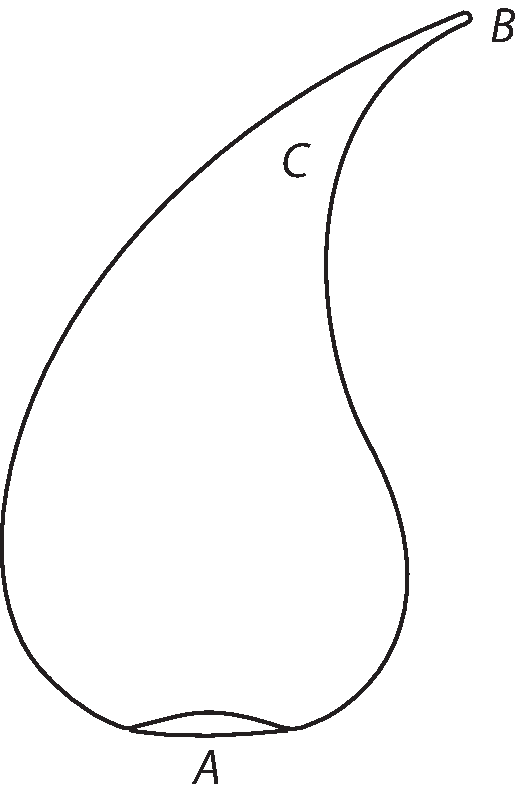
\includegraphics[trim = 0mm 0mm 0mm 0mm, clip, width=0.29\textwidth]{images//LH035,14,02_148r-d.pdf}\\
\noindent\centering [\textit{Fig. 5}]
\pend
\newpage
\pstart \noindent \textit{numeris foraminibus pervii.
Ubi rostrum paulo longius est, licet
\edtext{frangatur,}{\lemma{frangatur,}\Cfootnote{a.a.O.\cite{00044}, S.~324
mit Auslassungen: \textit{cucurbitula} [...] \textit{crepuit} und \textit{ivit;} [...] \textit{remansit}.}}}
si non attingatur bulla, vitrum non crepat.
Microscopio videbis bullam majorem in minore contineri; rostrum vero non esse perforatum. Summi caloris opera\protect\index{Sachverzeichnis}{opera caloris} cucurbitula candescens, non crepat, quamvis refrigeretur, observavi in aliqua bullulas summi caloris vi fere expunctas. In frangendo rostro sentitur magna resistentia, quae videtur non a vitro sed arcu quasi tenso se reducente. Saepe vitra sua sponte franguntur, ut mihi retulit Eustachius
Divini\protect\index{Namensregister}{\textso{Divini} (Divinus), Eustachio 1610-1685}, sibi nocte lentem in aliquot partes magno crepitu abiisse. \textit{Non raro evenit, dum infusa calida dolia purgantur, et abluuntur, ut obturamentum dolii post aliquot tempus non sine aliquo bombo avulsum eductumque avolet; et ne quis existimet ab halitu intus compresso extrudi, si dolium\protect\index{Sachverzeichnis}{dolium} subula perforetur, non quidem halitum\protect\index{Sachverzeichnis}{halitus} erumpentem, sed exteriorem aera exuctum cum solito sono adstantes audiunt. Igitur educitur obturamentum ab aere per rimas\protect\index{Sachverzeichnis}{rima} seu marginem foraminis exucto, sic corpus uliginosum inter digitos pressum, v.g. nucleus cerasi procul \edtext{emittitur.}{\lemma{emittitur.}\Cfootnote{a.a.O.\cite{00044}, S. 325.}}} \edtext{Porro}{\lemma{\textit{emittitur.}}\Bfootnote{\textit{(1)}\ Effectus igitur bull \textit{(2)}\ Porro \textit{L}}} ex his patet effectum esse bullulis ascribendum. In bullulis\protect\index{Sachverzeichnis}{bullulum} autem esse humorem tensum seu dilatatum, hinc humorem exugit, hinc resistentia in frangendo sentitur, hinc suctus sonum aemulatur, hinc calor\protect\index{Sachverzeichnis}{calor} minuit, frigus\protect\index{Sachverzeichnis}{frigor} auget impetum. Nam compressio frigore, tensio calore imminuitur. Bullulas esse meatibus inter se commissas, hinc consensum, seu una rapita rumpi omnes, aere celeritate \edtext{irrumpente.}{\lemma{irrumpente.}\Cfootnote{a.a.O.\cite{00044}, S. 328.}}
\pend 
\pstart Adde analogum quiddam ut vis appareat aeris
gravitantis. Eustachius Divinus\protect\index{Namensregister}{\textso{Divini} (Divinus), Eustachio 1610-1685} ex canna seu fistula catapultae longioris, cujus cavitas accurate et diligenter tornata erat, et immissae glandi prorsus aequalis, adducto \textit{anhelitu, pilam prius immissam cum adducere vellet, tanto cum impetu adducta est, ut dentem \edtext{fregerit}{\lemma{fregerit}\Cfootnote{a.a.O.\cite{00044}, S. 329.}}} (+~nihil hoc novi, vide Digbaeum\protect\index{Namensregister}{\textso{Digby} (Digbaeus), Kenelm (1603-1665)}.
Sed haec
Honoratus\protect\index{Namensregister}{\textso{Fabri}, Honor\'{e} SJ 1607-1688}
\edtext{scripsit}{\lemma{scripsit}\Cfootnote{\textsc{H. Fabri}, \title{Dialogi physici}\cite{00187}, Lyon 1665, S.~208.}}
anno \edtext{[1665]}{\lemma{1656}\Bfootnote{\textit{L ändert Hrsg.}}}~+) Ratio est quia ubi \textit{anhelitu aeris
aliquid adductum est, quod in canna remanet, tensum est, et dilatatum et proinde levius,} ergo \textit{per illud foramen, quod focum vulgo} vocant, \textit{totus aeris
cylinder cujus basis ori fistulae aequalis est suo pondere summam vim exerit, et pilam extrudit. Vitri\protect\index{Sachverzeichnis}{durities vitri} \edtext{durities}{\lemma{durities}\Cfootnote{\textsc{H. Fabri}, \title{Physica}\cite{00044}, Bd. 1, Lyon 1669, S. 329.}}} porro in experimento nostro \textit{ad rem non facit, quamquam eam aliqua stibii\protect\index{Sachverzeichnis}{admixtio stibii} \edtext{admixtio}{\lemma{admixtio}\Cfootnote{a.a.O.\cite{00044}, S. 329.}}} ut in aere campano conciliare possit. Adde temperaturam ut in ferro\protect\index{Sachverzeichnis}{ferrum}. (+ Ratio \edtext{cur raritas}{\lemma{cur}\Bfootnote{\textit{(1)}\ rariscentia \textit{(2)}\ raritas \textit{L}}} \edtext{minuat tensionem}{\lemma{minuat}\Bfootnote{\textit{(1)}\ dilatationem \textit{(2)}\ tensionem, \textit{L}}}, densitas compressionem, est NB. haec quod ex statu violento faciunt naturalem. +) Fractio vitrorum\protect\index{Sachverzeichnis}{fractio vitrorum} subitanea forte ab aliqua latente bulla tandem longo aeris molimine aperto procedit. \textit{Infusa calida} aer dolio contentus rarescit, \textit{obstructo foramine aer adduci nequit, hinc} adducto paulatim perrimas tandem operculum ejicitur. Modum fatetur sibi ignotum esse, quo ab artificibus talia vitra parentur (+ constat hodie esse quod vitrum instillatur aquae ex igne +). Vale scribebam 10. Kal. Jun. \edtext{1656.}{\lemma{1656.}\Cfootnote{a.a.O.\cite{00044}, S. 330.\hspace{-0.5mm}}}
\pend 
\pstart \textso{Hon. Fab. tract.} \pgrk{F}\,\textso{ys. 2. lib. 1. hypoth. 2.}
\textit{Extincto subito igne, non sentitur millesima pars illius caloris quae \edtext{prius.}{\lemma{prius.}\Cfootnote{a.a.O.\cite{00044}, S. 334.\hspace{-0.5mm}}}}
\pend 
\pstart \textso{Hon. Fab. tract.} \pgrk{F}\,\textso{ys. 2. lib. 1. prop. 14} Purus cinis\protect\index{Sachverzeichnis}{cinis purus} lucutento igni admotus, vix tantulum \edtext{incalescit.}{\lemma{incalescit.}\Cfootnote{a.a.O.\cite{00044}, S. 339.\hspace{-0.5mm}}}
\pend
\pstart \textso{Hon. Fab. tract.} \pgrk{F}\,\textso{ys. 2. lib. 1. prop. 20} Agere actione communi voco, ita agere, ut totus effectus a singulis causis dependeat, et ita agat ignis\protect\index{Sachverzeichnis}{ignis calefaciens} \edtext{calefaciens.}{\lemma{calefaciens.}\Cfootnote{a.a.O.\cite{00044}, S. 342f.}}
\pend 
%\newpage
\pstart \textso{Hon. Fab. tract.} \pgrk{F}\,\textso{ys. 2. lib. 1. prop. 34.} Ignis est causa primaria \edtext{caloris, hinc}{\lemma{caloris,}\Bfootnote{\textit{(1)}\ is \textit{(2)}\ hinc \textit{L}}} calor secundarius statim extinguitur igne \edtext{extincto.}{\lemma{extincto.}\Cfootnote{a.a.O.\cite{00044}, S. 348.}} At \edtext{cur durat calor in aqua}{\lemma{cur}\Bfootnote{\textit{(1)}\ in igne \textit{(2)}\ durat calor in aqua, \textit{L}}}, saxo, etc. quia in iis multis calor primarius intrusus; unde Scaliger\protect\index{Namensregister}{\textso{Scaliger}, Julius Caesar 1484-1558} agnoscit in aqua fervente ignem, ut et Sennertus\protect\index{Namensregister}{\textso{Sennert}, Daniel 1572-1637}. Minuitur calor dum divisione particularum ignis allapsis frigidis, tum avolatione\protect\index{Sachverzeichnis}{avolatio} earum cum \edtext{halitu.}{\lemma{halitu.}\Cfootnote{a.a.O.\cite{00044}, S. 350.}} Corpora sentiuntur calidiora inter quae plurimus ignis oleum calidius quam fervens aqua aurum liquatum quam aes, aes quam \edtext{plumbum.}{\lemma{plumbum.}\Cfootnote{a.a.O.\cite{00044}, S. 353.}} Eductio prop. 40. calor et potentia materiae est collectio \edtext{partium.}{\lemma{partium.}\Cfootnote{a.a.O.\cite{00044}, S. 354.}} Calor et lumen eodem modo diffunduntur, est enim lumen quidam calor \edtext{modificatus.}{\lemma{modificatus.}\Cfootnote{a.a.O.\cite{00044}, S. 355.}} Calor ita diffunditur praesertim in sublunaribus\protect\index{Sachverzeichnis}{sublunares}, ut cum eo multus halitus igneus conjunctus sit. Idem ait P. Aguillonius\protect\index{Namensregister}{\textso{Aguilon} (Aguillon, Aguilonius), Fran\c{c}ois de SJ 1661-1707}
lib. 5. optic. \edtext{def. 5.}{\lemma{def. 5.}\Cfootnote{\textsc{F. Aguilonius}, \title{Opticorum libri sex}\cite{00305}, Antwerpen 1613. S. 359.}} si vel subtilissimum velum luculento igni interponas vix calore senties. Hinc calor \edtext{noster vix}{\lemma{noster}\Bfootnote{\textit{(1)}\ non \textit{(2)}\ vix \textit{L}}} agit per refractionem\protect\index{Sachverzeichnis}{refractio} et reflexionem\protect\index{Sachverzeichnis}{reflectio} ut
\edtext{coelestis.}{\lemma{coelestis.}\Cfootnote{\textsc{H. Fabri}, \title{Physica}\cite{00044}, Bd. 1, Lyon 1669, S. 356f.}}
\textit{Flamma}
%
% \input{gesamttex/edit/LH035_14_02_148v.tex}
%
[148~v\textsuperscript{o}]
\textit{longius diffundit calorem quam carbo \edtext{accensus}{\lemma{accensus}\Cfootnote{a.a.O.\cite{00044}, S. 357.}}}, quia plus partium accensum est. Vitis et olea flammam luculentiorem nutriunt, quia plus in iis uliginis seu ignis. \textit{Aqua calida stanneo vasi probe obstructo \edtext{inclusa}{\lemma{inclusa}\Cfootnote{a.a.O.\cite{00044}, S. 358.}}} aliquot horis calorem servat. Haec vasa \textit{vulgo adhibentur ad conciliandum \edtext{calorem}{\lemma{calorem}\Cfootnote{a.a.O.\cite{00044}, S. 358.}}}, quippe satis moderatum febri correptis tempore horroris\protect\index{Sachverzeichnis}{tempus horroris}. Corpora incalescunt per affrictum ut serra, percussionem, ut malleus, unde non raro ignis percussione exilit, \textit{pressione, sic funis a gravi pondere tensus, et maxime ad trochleam\protect\index{Sachverzeichnis}{trochlea} \edtext{pressus}{\lemma{pressus}\Cfootnote{a.a.O.\cite{00044}, S. 359.}}}. Quia ubicunque humoris particulae motu separantur, id avolent, sequitur contra partium ignis quippe uliginosarum collectio\protect\index{Sachverzeichnis}{collectio uliginosarum} seu calor, (+ NB. nondum capio quod partes uliginosae sint rarefactivae +) vulgo dicunt incalescere sagittam motu per aerem hoc experientia comprobare non potui, imo appulsus aeris facit frigus. \textit{Animal motu incalescit}, quia agitatio fibras musculorum\protect\index{Sachverzeichnis}{agitatio musculorum} divellit, ut humor exprimatur, calor vitalis\protect\index{Sachverzeichnis}{calor vitalis} colligatur. \textit{Calor vitalis mirificam habet originem nempe tot percolationes in corpore animato fiunt, ut \edtext{secretis}{\lemma{secretis}\Cfootnote{a.a.O.\cite{00044}, S. 359 mit Auslassung: \textit{originem} [...] \textit{nempe}.}}} humidis ignis particulae colligantur. NB. \textit{Calor aquarum thermalium vel est ab ignibus subterraneis\protect\index{Sachverzeichnis}{ignis subterraneus}, vel ab eadem percolatione\protect\index{Sachverzeichnis}{percolatio}. Calor febris immoderatus internus quidem ideo accenditur, quod sanguinis arteriosi\protect\index{Sachverzeichnis}{sanguis arteriosus} \edtext{percolatio}{\lemma{percolatio}\Cfootnote{a.a.O.\cite{00044}, S.~359 mit Auslassungen: \textit{subterraneis, vel} [...] \textit{ab} und \textit{percolatione.} [...] \textit{Calor}.}}}
obstructione impediatur, unde non mirum si sanguis quasi 
\textit{in intimis praecordiis effervescat, externus quod tandem superata obstructione fractoque obice in exteriores} \edtext{[\textit{partes}]}{\lemma{\textit{partes}}\Bfootnote{\textit{erg. Hrsg. nach Vorlage}}}
\textit{quasi torrens \edtext{exundet}{\lemma{exundet}\Cfootnote{a.a.O.\cite{00044}, S. 359.}}} caloris virtualis eadem ratio, qui calefacit certo partium dispositione, v.g. piper attritum, vinum haustum quia saliva\protect\index{Sachverzeichnis}{saliva} devehit ignem liberatum in fibras subtilissiores etc. Unde piperis acrimonia, vini calor in stomacho ab humore separatur, \textit{si aqua calida primo soli admoveatur deinde removeatur \edtext{facilius}{\lemma{facilius}\Cfootnote{a.a.O.\cite{00044}, S. 360.}}} frigescit. Quia vis solis\protect\index{Sachverzeichnis}{vis solis} extrahere facit halitum igneum\protect\index{Sachverzeichnis}{halitus igneus}: aestus aestivus non est solum a radio perpendiculari magis, quia is et hyeme excipi plano obliquo potest, sed quia tunc in aere sunt innumerae ignis particulae\protect\index{Sachverzeichnis}{particulae ignis} calorem augentes, ut multi ignes positi in una linea \edtext{recta.}{\lemma{recta.}\Cfootnote{a.a.O.\cite{00044}, S.~361.}}
[146~r\textsuperscript{o}]
\pend% 
\pstart%
%
%
%
% \input{gesamttex/edit/LH035_14_02_146r.tex}
% [146~r\textsuperscript{o}]
\textso{Hon. Fab. Phys. Tract. 2. lib. 2. def. 1.} Frigus\protect\index{Sachverzeichnis}{frigus} est qualitas condensativa. \textso{Prop. 32.} Frigus frigefacit dividendo partes calidi\protect\index{Sachverzeichnis}{partes calidi} seu igneas\protect\index{Sachverzeichnis}{partes igneas}. Unde \textit{corpus frigefactivum ejus naturae esse debet, ut vel subtilia evibret corpuscula, vel constet illis partibus quae facile se \edtext{insinuent.}{\lemma{insinuent.}\Cfootnote{a.a.O.\cite{00044}, S. 371.}}} Eas partes seu id corpus vocat humorem purum\protect\index{Sachverzeichnis}{humor purus}, seu aquam puram, quae cum sit gravior igne eum elidit, et dividit, et \edtext{expellit.}{\lemma{expellit.}\Cfootnote{a.a.O.\cite{00044}, S.~373.}}
% \edtext{}{\lemma{expellit.}\Cfootnote{Fortsetzung in LSB VI, 2, S. 200.}}
Aqua calida mixta calidae aequalis gradus nec magis nec minus incalescit, mixta frigidae vel minus calidae frigescit, et illam frigefacit (+ par videtur ratio esse, si duo aeres compressi misceantur, item si compressus dilatato, et si compressus minus compresso. Sed in agendo discrimen est, quod totum compressum uno impetu in unum punctum agit, calor non agit NB. +) 
\textit{In qua proportione agat calidum in frigidum} et contra fuse dicemus tractatu \textit{4. est enim res scitu dignissima, quam vix ulla hactenus delibavit, nedum demonstravit.} Aer est frigidus\protect\index{Sachverzeichnis}{aer frigidus} quia subtilis et gravior igne (+ deberet etiam subtilior esse +) frigidior est cum a partibus igneis \edtext{liberior.}{\lemma{liberior.}\Cfootnote{a.a.O.\cite{00044}, S.~375.}} Unde aer afflatus frigefacit. Sed ille Mercurius\protect\index{Sachverzeichnis}{mercurius} tamen seu subtilis humor majorem ipso aere ad insinuandum se vim habet. \textit{Hinc nubecula hyeme frigidissima \edtext{sentitur}{\lemma{sentitur}\Cfootnote{a.a.O.\cite{00044}, S.~377.}}} innumeris humoris subtilis particulis constat, contra aestate\protect\index{Sachverzeichnis}{aestas} halitibus igneis unde si dissipata pomeridianum aestum facit majorem. Unde hyeme\protect\index{Sachverzeichnis}{hyems} saevit frigus, quia tunc ob obliquam solis actionem\protect\index{Sachverzeichnis}{actio solis} plus humoris subtilis quam halitus igni \edtext{educitur.}{\lemma{educitur.}\Cfootnote{a.a.O.\cite{00044}, S.~377.}} Quia ad pinguiorem partem seu halitum igneum educendum \edtext{fortissimo}{\lemma{educendum}\Bfootnote{\textit{(1)}\ multo \textit{(2)}\ fortissimo \textit{L}}} calore opus ut in distillatione patet. Aestate summa aeris regio frigidissima est, quia igneae particulae\protect\index{Sachverzeichnis}{particulae igneae} aqueas (sulphur\protect\index{Sachverzeichnis}{sulphur} mercurium\protect\index{Sachverzeichnis}{mercurius}) sursum expellunt, hinc et major hic aestus et illic frigus, hinc in inferiore fulgura et \edtext{tonitrua.}{\lemma{tonitrua.}\Cfootnote{a.a.O.\cite{00044}, S.~377f. (prop. 49).}} \textit{Dum aestate foris pluit intus fervet \edtext{aestus,}{\lemma{aestus,}\Cfootnote{a.a.O.\cite{00044}, S.~378.}}} quia aer pluviis densatus attrahit subtilis humoris\protect\index{Sachverzeichnis}{humor subtilis} particulas ex conclavibus, unde magis intus colliguntur pingues. Pluvia temperat aestum, quia halitum igneum dividit. Aqua cum impetu afflata plurimum frigoris conciliat, hinc \textit{ex siphone\protect\index{Sachverzeichnis}{sipho} \edtext{illo quem syringa\protect\index{Sachverzeichnis}{syringa} vocant}{\lemma{}\Bfootnote{\textit{illo quem syringa vocant} \textit{erg.} \textit{L}}} intruso embolo \edtext{evibrata}{\lemma{evibrata}\Cfootnote{a.a.O.\cite{00044}, S.~378.}}} frigidior sentitur et ideo magis ad ignem extinguendum adhibetur. Carbo\protect\index{Sachverzeichnis}{carbo} accensus aeri expositus citius in parte superiore extinguitur, quia facilius eo aer recta quam in inferiora oblique penetrat. Cinere\protect\index{Sachverzeichnis}{cinis} obtectus diu accensus manet, quia cinis \mercury\textsuperscript{rium}\protect\index{Sachverzeichnis}{mercurius} retinet et exugit. \textit{Carbo accensus citius hyeme quam aestate extinguitur sub \edtext{dio}{\lemma{dio}\Cfootnote{a.a.O.\cite{00044}, S.~379.}}}. Sed tamen semiaccensus a patulo aere melius accenditur ob venti appulsum. Nix est frigida quia multum 
\edtext{\mercury\ semper emittit}{\lemma{\mercury}\Bfootnote{\textit{(1)}\ continet \textit{(2)}\ semper emittit \textit{L}}} ruptis catervatim ignis actione bullis. Unde ventus e montibus nive\protect\index{Sachverzeichnis}{nix montium} tectis frigidissimus. Hac emissione nix aquam vinum\protect\index{Sachverzeichnis}{vinum}, fructus\protect\index{Sachverzeichnis}{fructus}, \edtext{refrigerat.}{\lemma{refrigerat.}\Cfootnote{a.a.O.\cite{00044}, S.~380.}} Hinc \textit{vitrei scyphi\protect\index{Sachverzeichnis}{scyphum vitreum} sudor in superficie externa dum aqua frigida vel vino frigido \edtext{impletur,}{\lemma{impletur,}\Cfootnote{a.a.O.\cite{00044}, S.~381.}}} quia halitus ambiens frigore concrescit, ut sudat marmor\protect\index{Sachverzeichnis}{sudor marmoris} afflante austro qui multum vaporem\protect\index{Sachverzeichnis}{vapor} vehit, itemque vitrei seu speculares\protect\index{Sachverzeichnis}{speculares} cancelli qui fenestras\protect\index{Sachverzeichnis}{fenestra} muniunt, quorum contra interna superficies\protect\index{Sachverzeichnis}{superficies interna} a frigore externo\protect\index{Sachverzeichnis}{frigor externo} sudat
\textit{nec enim per medium vitrum ex libero \edtext{aere}{\lemma{aere}\Cfootnote{a.a.O.\cite{00044}, S.~381 mit Auslassung: \textit{vitrum} [...] \textit{ex}.}}} humor subit, unde in cubiculis\protect\index{Sachverzeichnis}{cubiculum} ubi nemo habitat hoc non sentitur. Hyeme concrescit is \textit{halitus non modo in rorem sed in \edtext{gelu\protect\index{Sachverzeichnis}{gelu}}{\lemma{gelu}\Cfootnote{a.a.O.\cite{00044}, S. 381.}}} in levigata vitri\protect\index{Sachverzeichnis}{levigata vitri} superficie, at in asperiore chartae quae ex filaminibus constat, concrescit in \edtext{nivem, et}{\lemma{nivem}\Bfootnote{\textit{(1)}\ . Unde \textit{(2)}\ , et \textit{L}}} analogiam \textit{habes in brumali nubecula\protect\index{Sachverzeichnis}{nubecula brumalis} cujus filamina aliis corporibus implexa in nivem concrescunt,} unde et anhelitus\protect\index{Sachverzeichnis}{anhelitus} in barbae pilis concrescit in nivem. Nitrum\protect\index{Sachverzeichnis}{nitrum} emittit plurimum frigidi \mercury\textsuperscript{ii}. Aqua calida\protect\index{Sachverzeichnis}{aqua calida} agitata citius frigescit quia dividuntur ita et exhalant ignis \edtext{particulae}{\lemma{particulae}\Cfootnote{a.a.O.\cite{00044}, S.~382 (prop.~62).}} (+ quomodo leviores, si densiores et pinguiores, et quomodo sic rarefaciunt~+).
\textit{Irrigantur vici et conclavia ad temperandum aestum.} At modica irrigatio\protect\index{Sachverzeichnis}{irrigatio} magis promovet aestum, quia solum non penetrat, ideo superiorem superficiem quae magis adusta est tantum solvit ejusque partes igneas\protect\index{Sachverzeichnis}{partes igneae} secum elevat. Solum irrigatum exsiccatur scil. propter humoris irrigantis a sole elevationem, et quia inde sentitur odor\protect\index{Sachverzeichnis}{odor} quispiam isque parum gratus (+ imo qualis cretae, satis gratus~+). \textit{Aqua putealis aestate frigidior est, hyeme calidior,} quia hyberno frigore constricta terra\protect\index{Sachverzeichnis}{terra constricta} non avolat igneus halitus, aestate \edtext{avolat.}{\lemma{avolat.}\Cfootnote{a.a.O.\cite{00044}, S.~383 (prop. 64).}} Marmor frigidum quia in eo, ut aliis perfecte mixtis particulae ignis\protect\index{Sachverzeichnis}{particulae ignis} et humoris\protect\index{Sachverzeichnis}{particulae humoris} valde divisae, unde hae in illas agunt, et eas expellunt (+ at cur non potius humidae expellunt ignem, quippe graviores et subtiliores. +) constat autem marmor prae aliis lapidibus succo lapidescente\protect\index{Sachverzeichnis}{succus lapisdiscentis} probe \edtext{percolato.}{\lemma{percolato.}\Cfootnote{a.a.O.\cite{00044}, S.~383f. (prop. 65).}} Idem de metallis\protect\index{Sachverzeichnis}{metalla} politum est frigidius quia tunc pori minus obstructi. Hinc glacies frigidior nive. Imo in ferro\protect\index{Sachverzeichnis}{ferrum politum} polito et magnete  \edtext{levigato\protect\index{Sachverzeichnis}{levigatum magnetum}, et succino lacca\protect\index{Sachverzeichnis}{lacca}, etc. frictis vis\protect\index{Sachverzeichnis}{vis frictis}}{\lemma{levigato, et}\Bfootnote{\textit{(1)}\ electro fricto \textso{vis} \textit{(2)}\ succino lacca, etc. frictis vis \textit{L}}} major. Charta marmori levigato imposita tantulum humectata reperitur per \edtext{noctem.}{\lemma{noctem.}\Cfootnote{a.a.O.\cite{00044}, S. 383f.}} Aedes\protect\index{Sachverzeichnis}{aedes} ex levigato marmore \edtext{frigidiores.}{\lemma{frigidiores.}\Cfootnote{a.a.O.\cite{00044}, S.~384f. (prop.~68).}}
(+~Si qualibet nocte sensibilis emittitur humor,
cum possit ponderari; necesse est anno emitti dimidiam et ultra marmoris partem.
Ergo rectius aer per poros transit, quasi per angiportas~+). Hinc et humiditati obnoxiae\protect\index{Sachverzeichnis}{obnoxiae}, et frigidissima aura\protect\index{Sachverzeichnis}{aura frigidissima} ad limen\protect\index{Sachverzeichnis}{limen} offeretur intranti. Omne frigus humidum \edtext{est.}{\lemma{est.}\Cfootnote{a.a.O.\cite{00044}, S.~385 (prop. 69).}} Sal hyeme liquescit, imo et \textit{gluten, coagulum, saccaro condita, imo et caseus hyeme mollior} (+ ratio quia aer abit densatione\protect\index{Sachverzeichnis}{densatio} in aquam~+) \edtext{tela.}{\lemma{tela.}\Cfootnote{a.a.O.\cite{00044}, S.~385 (prop. 70).}} Si duas laevigati marmoris laminas, \textit{alteram candidi alteram nigri aestivo soli per aliquod tempus expones, et utramque manu} attrectabis, nigram senties calidissimam, candidum frigidum, nec recte dicetur omnia candida \edtext{temperamenti}{\lemma{temperamenti}\Cfootnote{a.a.O.\cite{00044}, S.~385 (prop. 71).}}
%
% \input{gesamttex/edit/LH035_14_02_146v.tex}
[146~v\textsuperscript{o}] 
%
frigidi esse, ecce enim arsenicum saccarum\protect\index{Sachverzeichnis}{saccarum arsenicum}, mercurius sublimatus\protect\index{Sachverzeichnis}{mercurius sublimatus}, adde puram flammam. Ratio igitur est, quod candida plus \edtext{lumen}{\lemma{}\Bfootnote{lumen \textit{erg.} \textit{L}}} reflectunt, ergo minus retinent. Hinc conclavia dealbata\protect\index{Sachverzeichnis}{conclavia dealbata} magis lumen reflectunt. Si lumen ergo \edtext{calorem.}{\lemma{calorem.}\Cfootnote{a.a.O.\cite{00044}, S. 385.}} Aqua est frigidior in \edtext{summo,}{{\lemma{}\Afootnote{\textit{Über} summo: \Denarius \vspace{-4mm}}}{\lemma{summo}\Cfootnote{a.a.O.\cite{00044}, S.~388.}}}\hfill et\hfill suprema\hfill eius\hfill superficies\hfill prius\hfill congelatur,\hfill \textit{quia\hfill in\hfill eam\hfill prae\hfill caeteris}
\pend
\newpage
\pstart
\noindent\textit{mercurius incubat.} Et ratio est quia mediae partis ignis dividitur \edtext{tantum a mercurio}{\lemma{tantum}\Bfootnote{\textit{(1)}\ ab igne ha \textit{(2)}\ a mercurio \textit{L}}} partis inferioris, summus a mercurio partis suae et inferioris configitur ergo quasi totidem \edtext{telis}{\lemma{telis}\Cfootnote{a.a.O.\cite{00044}, S.~388.}} (+ non omnia satis subito exhalare possunt, hinc congelantur.~+) Saeviente bruma maxime post nivem attrectatam incalescunt manus quia impeditur circulatio sanguinis\protect\index{Sachverzeichnis}{circulatio sanguinis}, hinc multus sanguis praesertim arteriosus\protect\index{Sachverzeichnis}{sanguis arteriosus} \edtext{colligitur.}{\lemma{colligitur.}\Cfootnote{a.a.O.\cite{00044}, S. 388f.}} \textit{Si manus maxime frigidas igni admoves, maximum dolorem \edtext{sentis}{\lemma{sentis}\Cfootnote{a.a.O.\cite{00044}, S. 389.}}} et semiusta parte igni admota major (+ puto minor, aliud si aquae admoventur +). Dolor\protect\index{Sachverzeichnis}{dolor} quia frigus \textit{per accidens partes ignis colligit,} unde novus calor accedens humorem facile educit, et ignem \edtext{auget}{\lemma{auget}\Cfootnote{a.a.O.\cite{00044}, S.~389.}}
(+~putarem potius motum obstructum violentius se exerere via facta~+).\textit{Congelata poma\protect\index{Sachverzeichnis}{poma} vel ova\protect\index{Sachverzeichnis}{ova} calidae immersa \edtext{corrumpuntur,}{\lemma{corrumpuntur,}\Cfootnote{a.a.O.\cite{00044}, S. 389.}}} quia glacies\protect\index{Sachverzeichnis}{glacies} est massa spumarum seu bullarum, non mirum ergo si congelata facile resolvat; \textit{si vero aquae frigidissimae immergantur integra deinde servantur, quia cum novi frigoris accessione magis densentur, nova illa condensatio foras exprimit mercurium congelativum\protect\index{Sachverzeichnis}{mercurius congelativus}, qui deinde ad instar glaciei extra adhaeret. Hinc Boreales\protect\index{Sachverzeichnis}{boreales}} quibus membra \edtext{hyberno itinere}{\lemma{hyberno}\Bfootnote{\textit{(1)}\ frigore \textit{(2)}\ itinere \textit{L}}} congelantur, non statim accedunt ad focum, ne summo dolore afficiantur, \edtext{\textit{sed membra}}{\lemma{\textit{sed}}\Bfootnote{\textit{(1)}\ \textit{manus} \textit{(2)}\ \textit{membra} \textit{L}}} \textit{gelidae immergunt,} non ut quod simile attrahat simile, \textit{ut vult }\textit{Sennertus}\protect\index{Namensregister}{\textso{Sennert}, Daniel 1572-1637}, sed quod gelida magis condensat, unde sequitur \edtext{expressio.}{\lemma{expressio.}\Cfootnote{a.a.O.\cite{00044}, S. 389.}} \textit{Frigus parens} \edtext{inertiae nam}{\lemma{inertiae}\Bfootnote{\textit{(1)}\ hinc \textit{(2)}\ nam \textit{L}}} stupefacit nervos, \textit{frigore manus et vultus lividum} \edtext{[\textit{colorem}]}{\lemma{calorem}\Bfootnote{\textit{L ändert Hrsg. nach Vorlage}}} \textit{contrahunt,
quia frigus constringit, hinc impedit sanguinis perlocationem\protect\index{Sachverzeichnis}{perlocatio sanguinis}, ac proinde sanguis collectus\protect\index{Sachverzeichnis}{sanguis collectus} hunc colorem} habet \textit{analogiam habes in contusa \edtext{carne.}{\lemma{carne.}\Cfootnote{a.a.O.\cite{00044}, S. 389.}}} Hinc et ob collecti sanguinis intumescentiam inflantur, imo finduntur, humore nimio plus aequo tensae, hinc vulnera\protect\index{Sachverzeichnis}{vulnera} in frigido difficilius curantur, quia coeunt calore partes opera filaminum, \textit{quae quasi faciunt stamen vitae, haec} autem filamina non nisi caloris opera duci possunt. Medicamenta\protect\index{Sachverzeichnis}{medicamentorum actio} quoque \textit{non agunt nisi per \edtext{corpuscula,}{\lemma{corpuscula,}\Cfootnote{a.a.O.\cite{00044}, S. 390.}}} et ita indigent calore ut educantur, frigus etiam stringit partes ita benignus calor et partis laesae restaurator excluditur. Hinc frigus sanguinem sistit, quia stringit meatus. Pallorem facit, quia stringendo sanguinis affluxum prohibet. Sic et stringendo lacrymas\protect\index{Sachverzeichnis}{lacrymae} provocat et nares\protect\index{Sachverzeichnis}{nares} stillare facit et compressione vel constrictione \textit{intestina ad egestionem solicitat, et post pastum \edtext{hyeme}{\lemma{hyeme}\Cfootnote{a.a.O.\cite{00044}, S. 390.}}} major horror, \textit{vulgo vitulina febris\hfill quia\hfill primae\hfill alimenti\hfill particulae\hfill paulo\hfill crudiores\hfill capillares\hfill venas\protect\index{Sachverzeichnis}{venae capillares}\hfill obstruunt.}
\pend
\newpage
\pstart
\noindent\textit{Hinc sanguis arteriosus\protect\index{Sachverzeichnis}{sanguis arteriosus} percolari non potest, nex ad partes externas \edtext{appelli,}{\lemma{appelli,}\Cfootnote{a.a.O.\cite{00044}, S. 390.}}} adde divisionem ignis per haec corpuscula quae ciborum \mercury\textsuperscript{ium}\protect\index{Sachverzeichnis}{cibus mercurius} appellare queas. Febris accessio\protect\index{Sachverzeichnis}{accessio febris} facit frigus, quia materia morbifica\protect\index{Sachverzeichnis}{materia morbifica} obstructione sanguinis percolationem impedit; \textit{timor\protect\index{Sachverzeichnis}{timor} etiam frigus et horrorem\protect\index{Sachverzeichnis}{horror}} facit, movet in sanguinem ad centrum. Hyeme plus edimus, quia non tot bilis seu sulphuris vel caloris resolutorii partes\protect\index{Sachverzeichnis}{partes bilis}\protect\index{Sachverzeichnis}{partes sulphuris}\protect\index{Sachverzeichnis}{partes caloris} exhalantur. \textit{Hinc animalia hyeme \edtext{pinguiora}{\lemma{pinguiora}\Cfootnote{a.a.O.\cite{00044}, S. 390 mit Auslassung \textit{animalia} [...] \textit{hyeme}.}}} (nisi scillicet iis nutrimentum\protect\index{Sachverzeichnis}{nutrimentum} desit, ut lupis). Hyeme humor per nares\protect\index{Sachverzeichnis}{nares} distillat, quia non potest abire per sudorem\protect\index{Sachverzeichnis}{sudor}, et exprimitur, hyeme manus congelatione laeduntur, quia congelatum facilius \edtext{frangitur,}{\lemma{frangitur,}\Cfootnote{a.a.O.\cite{00044}, S.~390.}} macilentis et rarae texturae hominibus frigus magis adversum, manus asperiores facilius frigore finduntur, \textit{quia sicciores, in pinguibus corpuscula frigida in intimas nervorum fibras\protect\index{Sachverzeichnis}{fibrae nervorum} non \edtext{penetrant.}{\lemma{penetrant.}\Cfootnote{a.a.O.\cite{00044}, S. 391.}}} Frigent magis qui nuper valetudinem recuperarunt. Pili\protect\index{Sachverzeichnis}{pilus} et villi\protect\index{Sachverzeichnis}{villus} optime frigus arcent, quia ignis filamina implicant, unde calorem diu servant, ergo et felinae pellis\protect\index{Sachverzeichnis}{pellis felinae} affrictu noctu scintillae excutiuntur. \textit{Vas figlinum aquam frigidam continens si diu pavimento vel laterculo incumbatur sensibile vestigium \edtext{relinquit,}{\lemma{relinquit,}\Cfootnote{a.a.O.\cite{00044}, S.~391 mit Auslassung: \textit{vestigium} [...] \textit{relinquit}.}}
quia praedicta corpuscula vas ipsum penetrant, et deorsum facilius quam sursum eunt. Si glacies imponatur orbi stanneo, et hic vitreo scypho\protect\index{Sachverzeichnis}{scyphus vitreus}, ad basin scyphi aqua congelatur quia mercurius\protect\index{Sachverzeichnis}{mercurius} ille facile \edtext{descendit}{\lemma{descendit}\Cfootnote{a.a.O.\cite{00044}, S.~391 mit Auslassung: \textit{eunt.} [...] \textit{Si}.}}} per
scyphum seu quasi serpit. Pili frigore rigescunt, quia contrahuntur pori\protect\index{Sachverzeichnis}{pori}, jam contractione apothecae\protect\index{Sachverzeichnis}{apotheca} cylinder infixus necessario erigitur, adde quod pili ipsi contrahuntur ergo rigescunt. Hinc si hyeme pectimus caput\protect\index{Sachverzeichnis}{caput} dolorem quasi in pilis sentimus quia ridigi difficilius inflectuntur, \textit{nisi vis fibris, quibus radices pilorum\protect\index{Sachverzeichnis}{radices pilorum} \edtext{adhaerent,}{\lemma{adhaerent,}\Cfootnote{a.a.O.\cite{00044}, S.~391.}}} inseratur. Senes frigidi, quia sicci membranosi et fibrosi, qualia frigida. \textit{Horrescimus affusa etiam calida, quia haec cuti adhaerens dividit partes ignis. Hyeme magis rigemus cum \edtext{currimus,}{\lemma{currimus,}\Cfootnote{a.a.O.\cite{00044}, S.~391 mit Auslassung: \textit{ignis.} [...] \textit{Hyeme}}}} non quia ob motum afflatus aer novum facit frigus, alioqui etiam rheda cito vectis fieret, sed quia fibrae quae rigori famulantur, jam a frigore ad rigorem\protect\index{Sachverzeichnis}{rigor} \edtext{determinatae, secundo motu}{\lemma{determinatae,}\Bfootnote{\textit{(1)}\ secunda vice \textit{(2)}\ secundo motu \textit{L}}} quasi \edtext{solicitantur.}{\lemma{solicitantur.}\Cfootnote{a.a.O.\cite{00044}, S.~391.}} \textit{Frigus non refringitur,} neque reflexitur, quia consistit in halitu corporeo\protect\index{Sachverzeichnis}{halitus corporeus}, quia modici nisus\protect\index{Sachverzeichnis}{nisus}, ut halitus odorifer\protect\index{Sachverzeichnis}{halitus odorifer} non reflectitur, nec refringitur, quia non transit \edtext{poros\protect\index{Sachverzeichnis}{pori}.}{\lemma{poros.}\Cfootnote{a.a.O.\cite{00044}, S.~391.}} Frigus sola attrectatione sentitur, non ut calor e longinquo. Corpuscula enim frigus facientia haerent superficiei, ut rubigo ferro\protect\index{Sachverzeichnis}{ferrum rubigum}, scabies cuti\protect\index{Sachverzeichnis}{scabies cuti}, furfur capiti\protect\index{Sachverzeichnis}{furfur capiti}, gummi cortici\protect\index{Sachverzeichnis}{gummi cortici} aerugo \edtext{aeri}{\lemma{aeri}\Cfootnote{a.a.O.\cite{00044}, S.~392f.}} (+ unde et ex aqua non avolat quia in glaciem concrescat +). Agit omnia in orbem, sed debiliter. Frigora sunt ut quadrata \edtext{distantiarum.}{\lemma{distantiarum.}\Cfootnote{a.a.O.\cite{00044}, S.~394.}} Frigida non agunt actione communi, alioqui esset magnum frigus a toto mari \edtext{etc.}{\lemma{etc.}\Cfootnote{a.a.O.\cite{00044}, S.~395.}} (+ imo agunt, sed debiliter ad extra +) virtualiter frigida, ut lactuca plantago cicuta\protect\index{Sachverzeichnis}{lactuca cicuta}, quia frigus sentitur resolutione. Frigidi temperamenti cerebrum membranae ossa\protect\index{Sachverzeichnis}{ossa} partes spermaticae quia ob densitatem facile frigus recipiunt et \edtext{servant.}{\lemma{servant.}\Cfootnote{a.a.O.\cite{00044}, S. 395.}}
[145~v\textsuperscript{o}]
\pend%
\count\Bfootins=1200
\count\Cfootins=1100
\pstart%
%
%
%
% \input{gesamttex/edit/LH035_14_02_145v.tex}
% [145~v\textsuperscript{o}]
\textso{Hon. Fab. tract. 2. lib. 3. prop. 7.} refert sententiam cujusdam recentioris, qui lumen\protect\index{Sachverzeichnis}{lumen} explicat per systolen\protect\index{Sachverzeichnis}{systole} et diastolen\protect\index{Sachverzeichnis}{diastole}, id est intumescentiam\protect\index{Sachverzeichnis}{intumescenta corporis} et detumescentiam\protect\index{Sachverzeichnis}{detumescentia corporis} corporis lucidi. (+ Sed ego non video quomodo hoc sit possibile, nisi perpetua partium rei emmissione. Nam quae intumescere faciunt extrorsum tendunt, quae extrorsum tendunt abire conantur, quae abire conantur si non possunt abire non conantur ultra momentum. +) Effectus quem praestat lumen in corpore illuminato est tantum rarefactio   \edtext{per se}{\lemma{per se}\Cfootnote{a.a.O.\cite{00044}, S. 418.}}, nam quod luna\protect\index{Sachverzeichnis}{luna} humectat, fit quod calore solis\protect\index{Sachverzeichnis}{calor solis} reflexo particulae ab humiditate abripiuntur. Est autem rarefactio non major quam quae sufficiat ad visibilitatem, seu liberam radiorum \edtext{trajectionem.}{\lemma{trajectionem.}\Cfootnote{a.a.O.\cite{00044}, S. 419.}} Etiam in oculo\protect\index{Sachverzeichnis}{oculus} nil aliud praestat lumen, quam quod \edtext{rarefacit.}{\lemma{rarefacit.}\Cfootnote{a.a.O.\cite{00044}, S. 422.}} Nam \textit{retina ex ductili substantia cerebri contexta cum infinitis propemodum venulis et arteriolis facile \edtext{rarescit}{\lemma{rarescit}\Cfootnote{a.a.O.\cite{00044}, S.~423.}}}, hinc \textit{per rarefactionem explicantur subtilissimae fibrae, ex quibus retina\protect\index{Sachverzeichnis}{retina} constat, ac proinde cum ducantur a cerebro\protect\index{Sachverzeichnis}{cerebrum} per nervos opticos\protect\index{Sachverzeichnis}{nervi optici}, facile illa tensio, ille motus, illa affectio in cerebrum traducitur, si enim chordam tangis tota illico \edtext{tremit.}{\lemma{tremit.}\Cfootnote{a.a.O.\cite{00044}, S.~423.}}} Minus lucidum aliquid est \edtext{ob admixtum non lucidum.}{\lemma{ob}\Bfootnote{\textit{(1)}\ aliquid \textit{(2)}\ admixtum non lucidum. \textit{L}}} \hspace{-1.2mm}\edtext{}{\lemma{lucidum.}\Cfootnote{a.a.O.\cite{00044}, S.~432f.}} Ut calor, unde non consistit in intensione, sed extensione. \textit{Litheosphoros\protect\index{Sachverzeichnis}{litheosphorus} est lapis mineralis in agro Bononiensi vulgo nascens, qui recte calcinatus ut aiunt vel ustus et debito modo praeparatus, si primum soli exponatur tum deinde in obscuro conclavi aspiciatur, lumen emittit ad instar carbonis accensi, modico cinere\protect\index{Sachverzeichnis}{cinis} aspersi, sed hoc lumen sensim languescit, tandemque \edtext{deficit,}{\lemma{deficit,}\Cfootnote{a.a.O.\cite{00044}, S.~442f.}}} differt in eo ab his noctilucis, \textit{quod lumini expositus accendatur} (+ forte hoc in caeteris quoque~+). \textit{Alii dicunt vaporem subtilissimum aeri admixtum facile lucem concipere a sole, qui vapor luce concepta in poros lapidis calcinati subit, ibique frigore cogitur, et cum partibus perspicuis quae lapidi intersunt conjunctus, tandem lucidus \edtext{evadit.}{\lemma{evadit.}\Cfootnote{a.a.O.\cite{00044}, S.~443.}}} At contra concipit \edtext{[lucem]}{\lemma{lapidem}\Bfootnote{\textit{L ändert Hrsg. nach Vorlage}}} et \textit{in vitrea pyxide hermetice \edtext{sigillata,}{\lemma{sigillata,}\Cfootnote{a.a.O.\cite{00044}, S.~443f.}}} dicendum lapidem esse plenum igne\protect\index{Sachverzeichnis}{lapis ignis}, qui accendatur a sole. Praeparatio fit saepe repetita calcinatione, accenditur \edtext{non tamen}{\lemma{non tamen}\Bfootnote{\textit{erg. L}}} \textit{ad instar naphtae\protect\index{Sachverzeichnis}{naphta}}, nam ductiles radii, \textit{quod scilicet ductiles radii ignem conceptum in aere consequenti quasi insensibilis fomitis inflammatione introrsum \edtext{adducant;}{\lemma{adducant;}\Cfootnote{a.a.O.\cite{00044}, S.~444.}}} alioqui lapis ad nostrum quoque ignem accenderetur, quod non est. Si oculos proxime oculis admoveatur, senties calorem, si naribus odorem sulphureum\protect\index{Sachverzeichnis}{odor sulphureus}, si humore dissolvas 
\textit{senties teterrimum odorem, quasi ex nitro\protect\index{Sachverzeichnis}{nitrum sulphurum} sulphure et bitumine\protect\index{Sachverzeichnis}{bitumen} spirantem. Calore solis melius accenditur,} quia sol igneus \edtext{est.}{\lemma{est.}\Cfootnote{a.a.O.\cite{00044}, S.~444.}} In pyxide\protect\index{Sachverzeichnis}{pyxis opaca} opaca \edtext{accenditur.}{\lemma{accenditur.}\Cfootnote{a.a.O.\cite{00044}, S.~445.}} \textit{Ex parte perspicuus est} ex parte \edtext{opacus.}{\lemma{opacus.}\Cfootnote{a.a.O.\cite{00044}, S.~445.}} Lux non nisi in loco obscuro \edtext{videtur.}{\lemma{videtur.}\Cfootnote{a.a.O.\cite{00044}, S.~445.}} Per calcinationem seperatur humor aqueus non inflammabilis unde repeti debet. Etiam intus lucet et in nova superficie, etsi frangatur. Hinc quasi cinis\protect\index{Sachverzeichnis}{cinis} aspersus videtur dum sensim \edtext{extinguitur.}{\lemma{extinguitur.}\Cfootnote{a.a.O.\cite{00044}, S.~445.}} Majorem lucem praebere videtur evigilanti, adeo ut ab eo adhuc videatur cum aliis  \edtext{extinctus videtur.}{\lemma{extinctus videtur.}\Cfootnote{a.a.O.\cite{00044}, S.~445.}} Adde \textit{si quis per aliquod tempus oculos} \edtext{clauserit.}{\lemma{clauserit.}\Cfootnote{a.a.O.\cite{00044}, S.~446.}} \textit{Hinc matutino\protect\index{Sachverzeichnis}{tempus matutinum} tempore major apparet lux, tum quia serotinus aer\protect\index{Sachverzeichnis}{aer serotinus} multum halitum admixtum habet, quia radios puri \edtext{luminis}{\lemma{luminis}\Cfootnote{a.a.O.\cite{00044}, S.~446 mit Auslassung: \textit{habet,} [...] \textit{quia}.}}} detinet, tum quia oculos\protect\index{Sachverzeichnis}{oculi} est \edtext{praeparatior. Et}{\lemma{praeparatior}\Bfootnote{\textit{(1)}\ , hinc \textit{(2)}\ . Et \textit{L}}}
plus in eo aestivo tempore lucis sereno quam pluvio, \textit{lunari lumine non \edtext{accenditur.}{\lemma{accenditur.}\Cfootnote{a.a.O.\cite{00044}, S.~446 mit Auslassung: \textit{lumine} [...] \textit{non}.}}} \textit{Quo ditius exponitur majorem lucem \edtext{concipit.}{\lemma{concipit.}\Cfootnote{a.a.O.\cite{00044}, S. 447.}}} Magis accenditur recto quam obliquo solis radio\protect\index{Sachverzeichnis}{radius soli}, \textit{si nix vel \edtext{glacies}{\lemma{glacies}\Cfootnote{a.a.O.\cite{00044}, S.~447.}}} propius admoveatur facilius extinguitur ob emissum mercurium, ut et \textit{si tenui flatu perfletur. Aqua lapidi aspersa, citius sensim tamen \edtext{extinguitur,}{\lemma{extinguitur,}\Cfootnote{a.a.O.\cite{00044}, S.~447.}}} non ut carbo\protect\index{Sachverzeichnis}{carbo} accensus statim, quia aqua non statim in 
\textit{exiguos poros\protect\index{Sachverzeichnis}{pori exigui} subire \edtext{potest.}{\lemma{potest.}\Cfootnote{a.a.O.\cite{00044}, S.~447 mit Auslassung: \textit{poros} [...] \textit{subire}.}}} Carbo accensa in pyxide\protect\index{Sachverzeichnis}{pyxis} aerea statim extinguitur, quia halitus quem emittit in ipsum repercutitur unde dicitur vulgo flamma suffocari clausa. Quod longe aliam quam vulgo putant, quasi aer pabulum sit rationem \edtext{habet.}{\lemma{habet.}\Cfootnote{a.a.O.\cite{00044}, S.~447.}} Senescit tandem ut \textit{lucem amplius non concipiat,} diutius tamen alius alio vivit, prout plus materiae alius accendibilis habuit aut \edtext{amisit.}{\lemma{amisit.}\Cfootnote{a.a.O.\cite{00044}, S.~447f.}} Aquae immersus aliquandiu amittit virtutem, tandem \edtext{recuperat.}{\lemma{recuperat.}\Cfootnote{a.a.O.\cite{00044}, S.~448.}} Partes interiores si frangas \textit{aliquid pristinae virtutis habent, sic ferrum ubi rubiginem
\edtext{contraxit}{\lemma{contraxit}\Cfootnote{a.a.O.\cite{00044}, S.~448 mit Auslassungen: \textit{habent,} [...] \textit{sic ferrum} [...] \textit{ubi}.}}}
 perdit virtutem magneticam, \textit{quae cito reviviscit} (+~ambigue an sponte, an novo affrictu~+) si rubiginem \edtext{abigas.}{\lemma{abigas.}\Cfootnote{a.a.O.\cite{00044}, S. 448.}} Nimi calore debilitatur, ut ferrum magneticam virtutem candefactum amittit. Lumen a Litheosphoro\protect\index{Sachverzeichnis}{litheosphorus} procedens per vitrum refingitur omne enim lumen hoc patitur, etiam cicindelae\protect\index{Sachverzeichnis}{cicindelae}. Sunt granula quaedam instar floris in lapide, quae prae caeteris lucent, et sunt ab exudante vel expressa per calcinationem\protect\index{Sachverzeichnis}{calcinatio} subtili materia. Sunt qui affirmant retinam\protect\index{Sachverzeichnis}{retina} eodem modo lucem \edtext{concipere,}{\lemma{concipere,}\Cfootnote{a.a.O.\cite{00044}, S. 448.}} ut litheosphoron aliqui affirmant, quia
\textit{si chartam, in qua aliquid imaginis vel figurae descriptum sit fixis et immobilibus oculis aliquandiu intuearis, ita ut charta solem inter et oculum collocetur tum deinde in conclavi obscurissimo in chartam albam oculos defigas eam primo croceam\protect\index{Sachverzeichnis}{croceus} videbis, tum rubram mox puniceam\protect\index{Sachverzeichnis}{rubra punicea}, et fere omni colorum varietate depictam, tandemque imaginem priorem videbis, modo nigram, modo flavam, modo rectam, modo inversam \edtext{etc.}{\lemma{etc.}\Cfootnote{a.a.O.\cite{00044}, S. 449.}}} Sed si quid in charta depingeretur, videret et socius tuus, quod non est, nec potest in oculis suis lux videri. Et si supponatur pupilla\protect\index{Sachverzeichnis}{pupilla} ejusdem diametri lucem inversam non videbis, nempe cum eadem refractione radii ab imagine depicta in fundo retinae per crystallinum trajecti ad objectum terminantur et ab objecto ad retinam, est enim certissima refractionum regula, quod si vis pupillam\protect\index{Sachverzeichnis}{pupilla} dilatare \edtext{etiam imaginem}{\lemma{etiam}\Bfootnote{\textit{(1)}\ refractionem \textit{(2)}\ imaginem \textit{L}}} rectam videbis, sed majorem, ut constat ex regulis opticis, et nos suo loco \edtext{demonstrabimus.}{\lemma{demonstrabimus.}\Cfootnote{a.a.O.\cite{00044}, S. 449f.}} Igitur apparet tantum, mihique ipsi contigit, ut cum legissem aliquid, et sex horas dormissem suavissimo somno\protect\index{Sachverzeichnis}{somnus}, ubi oculos aperui et in parietem ex opposito \textit{situm intendi eandem penitus scriptionem distinctis characteribus et verbis quasi in praedicto pariete exarata esset, distincte legi, brevissimo dumtaxat \edtext{tempore,}{\lemma{tempore,}\Cfootnote{a.a.O.\cite{00044}, S. 450.}}} nam statim evanuit. Sic phrenetici\protect\index{Sachverzeichnis}{phrenetici} ea vident, quae nunquam ante oculos habuerunt, \textit{quae insignes fibrarum cerebri\protect\index{Sachverzeichnis}{fibrae cerebri} mutationes patiuntur, quae in retinam traduci possunt.
Adde quod characteres seu notae coloris atri facile discernuntur seu a cerebro ad retinam
\edtext{traducuntur,}{\lemma{traducuntur}\Cfootnote{a.a.O.\cite{00044}, S.~451 mit Auslassung: \textit{possunt.} [...] \textit{Adde}.}}}
quia scilicet velut intactae relinquantur.
[144~r\textsuperscript{o}]
\pend%
\count\Cfootins=1200
\pstart%
%
%
%
% \input{gesamttex/edit/LH035_14_02_144r.tex}
% [144~r\textsuperscript{o}]
\textit{Lumen solis colores minus vegetos reddit, v.g. si peristromata\protect\index{Sachverzeichnis}{peristromata} vegetis tincta coloribus soli exponantur, pallescit color, quia calore solis
\edtext{subtilia}{\lemma{subtilia}\Cfootnote{a.a.O.\cite{00044}, S.~451
mit Aus\-lassungen: \textit{color,} [...] \textit{quia calore solis} [...] \textit{subtilia}.}}
corpuscula resolvuntur, quae lunam tingunt,
\edtext{hinc}{\lemma{hinc}\Cfootnote{a.a.O.\cite{00044}, S.~451
mit Auslassung: \textit{tingunt,} [...] \textit{hinc}.}}
panni tincti ita complicantur, ut lucem fugiant.
\edtext{Hinc}{\lemma{Hinc}\Cfootnote{a.a.O.\cite{00044}, S.~451
mit Auslassung: \textit{fugiant.} [...] \textit{Hinc}.}}
si diu subtiliores panni cancellis vitro} \edtext{[\textit{instructis}]}{\lemma{obstructis}\Bfootnote{\textit{L ändert Hrsg. nach Vorlage}}}
\textit{seu specularibus obducantur, ad mitigandam vim aestus, post aliquot annos vitrum eadem tinctura leviter tamen imbuitur, praesertim si color}
\edtext{[\textit{pannorum}]}{\lemma{\textit{pannorum}}\Bfootnote{\textit{erg. Hrsg. nach Vorlage}}}
\textit{sit vegetus\protect\index{Sachverzeichnis}{vegetus}, croceus\protect\index{Sachverzeichnis}{croceus}, rubeus\protect\index{Sachverzeichnis}{rubeus} etc.}
imo \textit{per poros subeunt vitri, totumque adeo vitrum}
\edtext{[\textit{leviter}]}{\lemma{leniter}\Bfootnote{\textit{L ändert Hrsg. nach Vorlage}}}
\textit{\edtext{inficiunt.}{\lemma{inficiunt.}\Cfootnote{a.a.O.\cite{00044}, S.~451.}}}
Retina rarefactionem et dilatationem a lumine facile recipit, quia ex ductili cerebri membrana, innumeris venis et arteriolis\protect\index{Sachverzeichnis}{venae arteriolae} quasi in rete quodam, unde retinae nomen, contexta est. Sed et uvea dilatatur ut videmus, quanquam potior retina. Ergo pupilla seu centrum uveae ipsa dilatata contrahitur lumine. Populorum septentrionalium visus hebes, quia inter perpetuas nives habitant quae lucem reflectunt, et oculos perstringunt; tum potius quia retina externo frigore induratur, imo \textit{frigus oculos ita stringit ut lacrymas \edtext{exprimat.}{\lemma{exprimat.}\Cfootnote{a.a.O.\cite{00044}, S. 452.}}} Adde quod \textit{cristallinus frigore concrescit, hinc flecti \edtext{nequit.}{\lemma{nequit.}\Cfootnote{a.a.O.\cite{00044}, S. 452.}}} Ophthalmia\protect\index{Sachverzeichnis}{opthalmia} efficit ut ophthalmici etiam modicam lucem fugiant
\textit{quia ophthalmia multam oculo inflammationem conciliat, sed retina ita affecta modico calore seu lumine plus aequo rarescit atque afficitur, nempe ex nimia tensione lacerantur et distrahuntur fibrae. Hinc ophthalmici ignem fugiunt, et frigida oculos abluunt, hinc destillatio\protect\index{Sachverzeichnis}{destillatio} vel defluvium\protect\index{Sachverzeichnis}{defluvium} oculi caloris
\edtext{excessum}{\lemma{excessum}\Cfootnote{a.a.O.\cite{00044}, S.~452 mit Aus\-lassungen: \textit{fibrae.} [...] \textit{Hinc} und \textit{abluunt,} [...] \textit{hinc}.}}}
notat, nam signum est, multum eo \edtext{[\textit{sanguinis}]}{\lemma{caloris}\Bfootnote{\textit{L ändert Hrsg. nach Vorlage}}} \textit{arteriosi confluere, cujus cum partes humoris percolatione separentur, partes ignis colligi necesse est, hinc tumor oculi ex sanguinis et humorum \edtext{appulsu.}{\lemma{appulsu.}\Cfootnote{a.a.O.\cite{00044}, S.~453 mit Auslassung: \textit{est,} [...] \textit{hinc}.}}} Per
quietem reficitur oculus per accessionem novarum partium quibus novum accidit luce affici, unde nictanti oculo lucem evigilantes intuemur, \textit{propter nimiam rarefactionem quae retinam afficit; ex qua distractio \edtext{fibrarum}{\lemma{fibrarum}\Cfootnote{a.a.O.\cite{00044}, S. 453 mit Auslassung: \textit{qua} [...] \textit{distractio}.}}} seu dolor. Unde et qui ex tenebris, diuturnis prodit, aegre lucem sustinet. Adde quod \textit{cum retina citius afficiatur quam uvea pupilla quae tunc explicatior est, nimiam lucem admittit, hinc nictatio\protect\index{Sachverzeichnis}{nictatio} et \edtext{dolor}{\lemma{dolor}\Cfootnote{a.a.O.\cite{00044}, S.~453.}}} adeo ut quidam ex diuturnis tenebris facti sint caeci, aut saltem hebetis visus retina frigore indurata, fibris diu in eodem situ haerentibus. Oculus fixus solem intueri vix potest propter nimiam luminis vim, et distractionem retinae, et quia lenticularis humoris\protect\index{Sachverzeichnis}{humor lenticularis} cristallini forma radios instar vitri ustorii colligit, adeo ut \textit{non semel adhibito bubulo cristallino perinde ac lente vitrea pulverem \edtext{tormentarium}{\lemma{tormentarium}\Cfootnote{a.a.O.\cite{00044}, S. 453.}}} incenderimus. Senum oculos lux minus afficit, quia habent retinam sicciorem, et ita minus flexibilem, nam sicca, ut testa\protect\index{Sachverzeichnis}{testa}, lateres\protect\index{Sachverzeichnis}{lateres}, ossa\protect\index{Sachverzeichnis}{ossa}, quae plus terrae habent, minus rarescunt. Adde quod sicciores particulae tot sanguinis percolationibus, quot in corpore humano fiunt colliguntur.
\pend 
\count\Afootins=1200
\count\Bfootins=1400
\count\Cfootins=1400
\pstart
\textit{Aliquando lucem de nocte evigilantes \edtext{vident,}{\lemma{vident,}\Cfootnote{a.a.O.\cite{00044}, S. 454.}}} non ab oculo emissam, unde circumferunt. Tiberii\protect\index{Namensregister}{\textso{Tiberius}, römischer Kaiser (14-37) 42 v. Chr. - 37. n. Chr.} oculos aliorumque lucem emisisse. Sed multos vidi quorum oculi lumen egregie reflecterent, quorum emitterent, nullum. Et quod feles ajunt noctu videre quia lucem emittant falsum est. Vident quodam tempore, et quaedam animalia noctu, quia retina ita praeparata, ut debilem lucem sentiat. Felem\protect\index{Sachverzeichnis}{felis} et noctuam in obscurissimo conclavi habui, nihil lucis vidi. Idem de vespertilionibus, imo cane\protect\index{Sachverzeichnis}{canis}, equo\protect\index{Sachverzeichnis}{equus}, bove\protect\index{Sachverzeichnis}{bovis}. Ita et somno, praeparari retina potest, quia et nimia luce perstringitur. Unde animalia\protect\index{Sachverzeichnis}{animalia} quae noctu vident die minus vident, quia enim parva lux iis ad visum sufficit, nimia minus sufficit et proinde nocet, unde iis dies pro somno. Ophthalmici quoque modica luce ad legendum indigent. In squamis quoque piscium lucem vidi, in oculis nunquam. Quod si qua lux talis sit, non retinae inerit sed uveae, vel certo humori corneam\protect\index{Sachverzeichnis}{cornea} inter et uveam\protect\index{Sachverzeichnis}{uves}, circa utriusque margines. Caetera cur evigilantes subitam lucem vident, potest et ut supra ab imaginatione proficisci. \edtext{Nonnunquam hebetiorem}{\lemma{Nonnunquam}\Bfootnote{\textit{(1)}\ qui \textit{(2)}\ hebetiorem \textit{L}}} visum habentibus ita subito acuitur visus, quanquam
\textit{brevi temporis spatio, ut distinctissime \edtext{videant,}{\lemma{videant,}\Cfootnote{a.a.O.\cite{00044}, S. 455.}}} quae prius confuse videre solebant. Necesse erat retinae subitam dispositionem accessisse \textit{a congestione particularum ignis, vel appulsu repentino subtilissimae \edtext{materiae.}{\lemma{materiae.}\Cfootnote{a.a.O.\cite{00044}, S. 456.}}} 
\textit{Ex oculi compressione lux emicat de noctu ad instar modici \edtext{fulgetri,}{\lemma{fulgetri,}\Cfootnote{a.a.O.\cite{00044}, S. 456.}}} quia retina compressa exprimuntur subtilissimae partes humoris et ignis \edtext{colligitur. De}{\lemma{colligitur.}\Bfootnote{\textit{(1)}\ Hinc \textit{(2)}\ De \textit{L}}} noctu tantum et in tenebris hoc lumen sentitur, et a me non aliis. De die lumen majus praevalet, ut hoc non sentiatur. \edtext{\textit{Hinc}}{\lemma{}\Bfootnote{\textit{Hinc} \textit{erg.} \textit{L}}}
\textit{fulgetrum apparet in parte oculi, non a qua sed versus quam fit \edtext{compressio.}{\lemma{compressio.}\Cfootnote{a.a.O.\cite{00044}, S. 456.}}} Hinc \textit{si capiti\protect\index{Sachverzeichnis}{caput} vel oculo ictus infligitur scintillas\protect\index{Sachverzeichnis}{scintilla}} emittere videtur agitatione illa humorum seu sanguinis arteriosi (+ \Denarius\ an et alliis appareat, et non puto +).
\textit{Scintillae\protect\index{Sachverzeichnis}{scintilla} ex affrictu felis\protect\index{Sachverzeichnis}{fel} in dorso\protect\index{Sachverzeichnis}{dorsum} emicare \edtext{videntur,}{\lemma{videntur,}\Cfootnote{a.a.O.\cite{00044}, S. 456.}}} quia frictu exprimitur humor, ergo partes igneae\protect\index{Sachverzeichnis}{partes igneae}, quarum magna in pellibus et pilis vis, maxime in felinis (+ quomodo cum pili praebeant tantum sal volatile +) nam in tanta pilorum sylva ignis implicatur. Imo \textit{scintillae avolant etiam ex ligno calefacto prius,} si postea succutiatur. \textit{Hinc si pellem igni admoveas,} maxime si ignis \edtext{[lignis]}{\lemma{}\Bfootnote{linis \textit{\ L \"{a}ndert Hrsg. nach Vorlage}}} resiniferis\protect\index{Sachverzeichnis}{lignum resinifere}; abie\protect\index{Sachverzeichnis}{abis}, pinu\protect\index{Sachverzeichnis}{pinus}, \edtext{alatur.}{\lemma{alatur.}\Cfootnote{a.a.O.\cite{00044}, S. 456.}} \textit{Probabile est illa animalcula} subtilia\protect\index{Sachverzeichnis}{animalcula subtilia} \textit{quae mixto insunt tantae parvitatis, ut oculos fugiant, si oculos habent, etiam de nocte videre,} et alioqui frustra oculos \edtext{haberent.}{\lemma{haberent.}\Cfootnote{a.a.O.\cite{00044}, S.~456 mit Auslassung: \textit{ut} [...] \textit{oculos}.}}
Illi optime vident quorum retina facile modico lumine afficitur, sed tamen \textit{talis est temperamenti,} ut etiam \textit{maximae luci \edtext{resistat}{\lemma{resistat}\Cfootnote{a.a.O.\cite{00044}, S. 456.}}} nec ut ea distrahatur. Multo igitur igne constare debet, sed praeparato et substantia solida. Tales falconum et aquilarum oculi qui et solem sine nictatione\protect\index{Sachverzeichnis}{nictatio}
%
% \input{gesamttex/edit/LH035_14_02_144v.tex}
[144~v\textsuperscript{o}]
%
\edtext{intuentur. \\ \indent Ratio}{\lemma{intuentur.}\Bfootnote{\textit{(1)}\ Lux solis \textit{(2)}\ Ratio \textit{L}}} cur animalia illa altivola\protect\index{Sachverzeichnis}{animalia altivola} tam acute videant, est ut praedam videant. Lux solis sternutationem\protect\index{Sachverzeichnis}{sternutatio} provocat, quia fibrae tenduntur, ut si quis nares intus pluma \edtext{vellicet.}{\lemma{vellicet.}\Cfootnote{a.a.O.\cite{00044}, S. 457f.}} Subrubram flammam praeferrunt quae multum fumi emittunt, intermixtis quasi umbellis, unde rubor. \textit{Aquae vitis flamma caerulea} est ab intermixto humore qui accendi nequit, unde et \textit{flamma cerae ad radicem coni caeruleum colorem \edtext{praefert}{\lemma{praefert}\Cfootnote{a.a.O.\cite{00044}, S. 458.}}} (+ Ergo nigrum luci mixtum est rubrum, perspicuum mixtum caeruleum\protect\index{Sachverzeichnis}{mixtum caeruleum} \Denarius\ +), \textit{itemque sulphuris flamma, si praedictae aquae aliquid aeruginis\protect\index{Sachverzeichnis}{aerugo} admisceas,} habebis 
\textit{virentem flammam, si cinnabarim\protect\index{Sachverzeichnis}{cinnabar}, rubeo colore} habebis. Hinc lignum siccum et cera alba puriorem lucem
\edtext{alunt}{\lemma{alunt.}\Cfootnote{a.a.O.\cite{00044}, S. 458f.}} \hspace{-1.2mm}\edtext{. Noctu}{\lemma{alunt.}\Bfootnote{\textit{(1)}\ Stellae \textit{(2)}\ Noctu \textit{L}}} lucentia magis videmus, quia nocte explicatur pupilla, unde lucem minorem facile recipit, die contrahitur. Hinc stellas\protect\index{Sachverzeichnis}{stellae} quoque de die non videmus quia contracta pupilla insensibilem tandem angulum faciunt, unde, si quis mane stellam fixo obtutu intueatur, continenter eam decrescere observabit, donec tandem ob parvitatem evanescat quia si quis dum \textit{venerem vel aliam illustrem stellam inspicit, cereum accensum oculo admoveat, statim eam imminui et tandem evanescere videbit, et si testem adhibeat, is pupillam\protect\index{Sachverzeichnis}{pupilla} contrahi \edtext{videbit,}{\lemma{videbit,}\Cfootnote{a.a.O.\cite{00044}, S. 459 mit Auslassung: \textit{videbit,} [...] \textit{et}.}}} lucerna admota. Hinc stellae videntur majores quam in tanta distantia. Qui ex illustri conclavi in obscuram transit, initio nihil videt, quae alii qui jam ibi fuere, quia vincit adhuc remanens impressio lucis prioris. Unde si claudatur oculus citius prior affectio deletur, et pupilla aperitur, et intus posita \edtext{videntur.}{\lemma{videntur.}\Cfootnote{a.a.O.\cite{00044}, S. 460.}} Hinc ratio patet cur identidem oculos claudamus, hinc suadeo debilem visum habentibus \textit{ut identidem dum legunt, oculos a libro avertant distrahant, claudant, et aliquandiu \edtext{relaxent.}{\lemma{relaxent.}\Cfootnote{a.a.O.\cite{00044}, S. 461.}}} Ab eo qui pupillam explicarit, et aliud lumen \edtext{excluserit, stellae videri possunt de die}{\lemma{excluserit,}\Bfootnote{\textit{(1)}\ de nocte \textit{(2)}\ stellae videri possunt de die. \textit{L}}}. Quod quomodo fieri debeat, viderint mechanici\protect\index{Sachverzeichnis}{mechanici}, 
\textit{certe si quis in altissimo puteo esset, et aliqua illustris \edtext{stella}{\lemma{stella}\Cfootnote{a.a.O.\cite{00044}, S. 461 mit Auslassung: \textit{esset,} [...] \textit{et}.}}} in illo coeli tractu esset, qui puteo responderet, stella videretur haud dubie. Adde et si tubus longus ad stellam dirigatur, sed hoc casu fieret, quia incerti sumus, quo dirigere debeamus. Ergo sane adhibitis testibus 
\textit{venerem aliquando a solis ortu usque ad \edtext{meridiem\protect\index{Sachverzeichnis}{meridies}}{\lemma{meridiem}\Cfootnote{a.a.O.\cite{00044}, S. 461.}}} vidi. 
\textit{Explicata pupilla} (+ vel quod idem est contracto oculo +)
\textit{majus lumen extensive et intensive in oculum incidit. Primum constat, quia lumen sub majore angulo appellitur, igitur \edtext{major}{\lemma{major}\Cfootnote{a.a.O.\cite{00044}, S. 462 mit Auslassung: \textit{incidit.} [...] \textit{Primum}.}}} eius quantitas, deinde quo major cristallini portio detecta est, radii in eum obliquius cadunt, igitur major est angulus refractionis\protect\index{Sachverzeichnis}{angulus refractionis}, igitur major angulus decussationis\protect\index{Sachverzeichnis}{angulus decussationis}, igitur major retinae portio afficitur (+ NB. retina est quasi paries, cristallinus quasi vitrum camerae obscurae\protect\index{Sachverzeichnis}{camera obscura} +). Porro est et majus lumen instensive, quia a singulis objecti punctis ad singula retinae detectae puncta radii ducuntur. Igitur plures radii ad idem retinae punctum determinabuntur. Hi \textit{radii qui ex lucerna distracti progredi \edtext{videntur,}{\lemma{videntur,}\Cfootnote{a.a.O.\cite{00044}, S. 462.}}} sunt ex reflexione ciliorum\protect\index{Sachverzeichnis}{reflexio ciliorum}. Hinc oculo omnino aperto non videntur, \textit{hinc cilia\protect\index{Sachverzeichnis}{cilia} quasi committuntur et palpebrae\protect\index{Sachverzeichnis}{palpebrae} ex parte clauduntur, hinc dum quis mane evigilat istud phaenomenon clarius videt, quia cilia uliginoso humore\protect\index{Sachverzeichnis}{humor uliginosis} per somnum collecto diluta sunt, atque adeo melius reflectunt, hinc videntur tremere illi radiii quia flamma lucernae tremulo motu subsultat, hinc curvi esse videntur, quia et cilia curva sunt, sunt demum duo radii propter duplicem ordinem \edtext{ciliorum.}{\lemma{ciliorum.}\Cfootnote{a.a.O.\cite{00044}, S. 462.}}} De hoc suo loco. Tersus oculus luci excipiendae aptior, explicantur enim tunica \textit{rugae, quae reflexionem impediunt. Hinc ebriorum oculi \edtext{micant,}{\lemma{micant,}\Cfootnote{a.a.O.\cite{00044}, S. 462.}}}\hfill turgent\hfill enim\hfill humoris\hfill appulsu,\hfill unde\hfill cornea\hfill magis\hfill
\textit{tenditur,\hfill fitque\hfill magis\hfill tersa,}
\textit{igitur melius reflectit, ira correptis idem \edtext{accidit,}{\lemma{accidit,}\Cfootnote{a.a.O.\cite{00044}, S. 462.}}} et laetis \textit{languent moerentibus et timentibus, quia humores concentrantur, hinc oculus minus plenus \edtext{flaccescit.}{\lemma{flaccescit.}\Cfootnote{a.a.O.\cite{00044}, S. 462.}}}
\pend
\count\Bfootins=1200
\count\Cfootins=1200 
\pstart\textit{Cicindelarum species\protect\index{Sachverzeichnis}{species cicindelarum} variae, aliae volantes aliae non volantes, volantes minores sunt et minus lucent idque quasi alternis scintillationibus, propter alarum motum, quas modo contrahunt modo explicant, dum explicant lux videtur, dum contrahunt obtegitur. Quae non \edtext{volant}{\lemma{volant}\Cfootnote{a.a.O.\cite{00044}, S. 463 mit Auslassung: \textit{obtegitur.} [...] \textit{Quae}.}}} majores sunt vel minores. Majores quasi erucae, minores frequentiores. Lux in extrema alvo (+ uti odor Zibeti\protect\index{Sachverzeichnis}{odor Zibeti} in testiculis\protect\index{Sachverzeichnis}{testiculus} +). \textit{Haec lux ab \edtext{igne,}{\lemma{igne,}\Cfootnote{a.a.O.\cite{00044}, S. 463.}}} collectis partibus per percolationem\protect\index{Sachverzeichnis}{percolatio}, optime in corpore animali ut constat, ex vitali calore. Continetur materia multis pelliculis\protect\index{Sachverzeichnis}{pellicula} quasi coagulatis, et etsi perenni effluvio abeant, restaurantur tamen ex excrementis animalis (+ NB. tentandum an animal diu vivum sustentari queat, et retineat semper lumen, deinde an inclusa materia vitro sigillato\protect\index{Sachverzeichnis}{vitrum sigillatum} lumen retineat +). Quando tangitur contrahit se et minorem lucem diffundit. Nam membranulam contrahit quae lucem tegit, etsi quidam putent a cicindela lucidam materiam introrsum adduci, si interfecta est nitedula, et \textit{spargitur in chartam materia lucens post aliquot dies sensim lucem \edtext{amittit;}{\lemma{amittit;}\Cfootnote{a.a.O.\cite{00044}, S. 463.}}} jucundum tamen visu est, si hac materia imaginea efformes in charta, ita figuram lucidam in tenebris aspicies. Lucet non urit, quia et debiliter lucet, ergo in tenebris lucet. Humor qui luceat ex cicindelis distillabilis nullus. Vix enumerari possunt pisces\protect\index{Sachverzeichnis}{pisces} quorum squamae lucent. Continent succum uliginosum\protect\index{Sachverzeichnis}{succus uliginosus}, \textit{hinc si squamam cultro vel vitro radas, vel ad ignem exicces, nullam lucem \edtext{emittit.}{\lemma{emittit.}\Cfootnote{a.a.O.\cite{00044}, S. 464.}}} Finis naturae est, \textit{ut ab aliis quibus infesti sunt, fugiantur, lucius enim qui hanc lucem prae caeteris habet,
est voracissimus sic lupus\protect\index{Sachverzeichnis}{lupus} animal terrestre,
non luce sed odore\protect\index{Sachverzeichnis}{odor} abigit
\edtext{oves.}{\lemma{oves.}\Cfootnote{a.a.O.\cite{00044}, S.~464 mit Auslassung: \textit{fugiantur,} [...] \textit{lucius}.}}}
Quaedam ostrea, quae Plinius\protect\index{Namensregister}{\textso{Plinius Secundus Maior}, Gaius 23-79} solenes appellat, succum habent lucentem, quo si vel manus, vel vultum ungas \edtext{lucet.}{\lemma{lucet.}\Cfootnote{\textsc{Plinius Secundus Maior}, \title{Historia naturalis}, XXXII, 53 (151).\cite{00306}}} In squamis ab intrinseco etiam praeparatione per corpus animalis\protect\index{Sachverzeichnis}{corpus animalis} \textit{exudat, hinc circa commissuras potissimum \edtext{lucet.}{\lemma{lucet.}\Cfootnote{\textsc{H. Fabri}, \title{Physica}\cite{00044}, Bd. 1, Lyon 1669, S. 464.}}} Lignum putridum sepultum esse oportet, nam si aere exponatur aliquandiu non amplius lucet (+ an retinet lucem, Hermetice sigillato in vase [+)]. Agaricum\protect\index{Sachverzeichnis}{agaricum} noctu lucet ob eandem rationem, est fungi\protect\index{Sachverzeichnis}{genus fungi} et plantae genus\protect\index{Sachverzeichnis}{genus plantae}, cum eo singularis percolatio\protect\index{Sachverzeichnis}{percolatio}, nam et magna vi corpus purgat, est ex parte dia\pgrk{f}anum. Luciola vel lingua serpentis, planta quae aliquid lucis scil. virtute vegetativa\protect\index{Sachverzeichnis}{virtus vegetativa} praeparatae emittit. \textit{Fluctus marini remo percussi, vel tempestatibus agitati debiliores scintillas\protect\index{Sachverzeichnis}{scintilla} emittunt. Constat enim aqua marina uligine \edtext{multa.}{\lemma{multa.}\Cfootnote{a.a.O.\cite{00044}, S.~465 mit Auslassung: \textit{tempestatibus} [...] \textit{agitati}.}}} \textit{Umbra
nucis\protect\index{Sachverzeichnis}{nux} dicitur capiti dolorem conciliare fraxineas umbras\protect\index{Sachverzeichnis}{umbra fraxinea} serpens\protect\index{Sachverzeichnis}{serpens} \edtext{fugit,}{\lemma{fugit,}\Cfootnote{a.a.O.\cite{00044}, S. 466 mit Auslassung: \textit{conciliare} [...] \textit{fraxineas}.}}} ut ajunt fraxinus sudorem exitat. Ratio non ab umbra sed corporum profluviis quae extra umbram sol discutit. Captamus umbram contra aestum, ergo laxioribus poris facilior passus, adde dormientes facilius affici, adde solum vel plantas ibi consitas saepe et corpuscula illa olfactu\protect\index{Sachverzeichnis}{olfactus} probamus. Adde proximas paludes\protect\index{Sachverzeichnis}{paludes}; fervens calor plura corpuscula excitat, aestu 
\textit{rarescit aer superior fitque levior, hinc corpuscula citius \edtext{descendunt.}{\lemma{descendunt.}\Cfootnote{a.a.O.\cite{00044}, S.~466.}}}
[143~v\textsuperscript{o}]
\pend%
\count\Bfootins=1200
\count\Cfootins=1200
\pstart%
%
%
%
% \input{gesamttex/edit/LH035_14_02_143v.tex}
% [143~v\textsuperscript{o}]
\textso{Hon. Fab. Phys. Tract. 2. lib. 4. prop. 1. et 2.} Humidum corpus seu quod quamlibet alterius figuram induat dari necesse est, ad replendos siccorum corporum hiatus. Alioqui quomodo corpus reperiemus quod angulo contingentiae commensuretur ad tollendum vacuum. Contra siccis opus est ad humida formanda et \edtext{continenda.}{\lemma{continenda.}\Cfootnote{a.a.O.\cite{00044}, S. 468.}}
\pend
\pstart \textso{Hon. Fab. Phys. Tract. 2. lib. 4. prop. 26.}
\textit{Humida in cumulum congeri non \edtext{possunt,}{\lemma{possunt,}\Cfootnote{a.a.O.\cite{00044}, S. 483.}}} sed quaerunt aequilibrium. \textso{Prop. }\edtext{[\textso{27.}]}{\lemma{\textso{28.}}\Bfootnote{\textit{L \"{a}ndert Hrsg. }}} Ignis non est humidus, sed siccus\protect\index{Sachverzeichnis}{ignis siccus}, nam etsi flexibilis, tamen resistit, si omnia flexibilia sunt humida, etiam filum \edtext{erit.}{\lemma{erit.}\Cfootnote{a.a.O.\cite{00044}, S. 484.}}
\pend 
\count\Bfootins=1200
\count\Cfootins=1200
\pstart \textso{Hon. Fab. Phys. Tract. 2. lib. 4. prop. 28.} Succus seu uligo seu pinguedo est ab igne humori mixto. Non ab aere, fabula enim est ignem aere ali, et certe alioquin totus aer tandem face admota accenderetur. In mixtis resolutis\protect\index{Sachverzeichnis}{mixta resoluta}, resolvitur terra in sal, aqua in mercurium, ignis in sulphur, aeris resolutio non est sensibilis. Corpora humana\protect\index{Sachverzeichnis}{corpora humana} his pinguibus optime nutriuntur quia optime nutriunt, quae facile neri possunt. Sulphur, seu succus est humidum igni \edtext{mixtum.}{\lemma{mixtum.}\Cfootnote{a.a.O.\cite{00044}, S. 486.}} Aridum dicit absentiam non tantum humoris, sed et \edtext{succi.}{\lemma{succi.}\Cfootnote{a.a.O.\cite{00044}, S. 487.}} Aqua stygia solvit tenuibus et acutis seu denticulatis quas vehit partibus, et rumpit partium filamina, quae ignis iterum \edtext{connectit}{\lemma{connectit}\Cfootnote{a.a.O.\cite{00044}, S. 487.}} (+ cur ergo fluentia in igne liquida et incohaerentia +). Oleum difficilius penetrat, nisi humore dilutum, ita vinum purum in mantili quasi in guttulas tornatur, ut dilutum statim per poros subit, idem accidit in vase hederaceo sed contra filamina faciunt, ut res diutius oleo madeat corpuscula autem illa corrodentia dura et sicca esse necesse \edtext{est.}{\lemma{est.}\Cfootnote{a.a.O.\cite{00044}, S. 488.}} Ergo potest siccum esse tenue, contra humidum potest esse crassum ita aqua multa terra, gypso, uligine diluta sanguis crassus qui difficulter per venas capillares percolatur. Ferrum est durius vitro, licet vitrum sit siccius friabilia facile, non dicimus \edtext{dura.}{\lemma{dura.}\Cfootnote{a.a.O.\cite{00044}, S. 489.}} Dura fortioribus filaminibus et pluribus unita. Ergo durum multo igne constat, sed et multa terra. Ita oleum est multi ignis, non durum tamen; durum ergo constat multo igne, et multa terra ignem dividente, unde dura frigida, plumbum\protect\index{Sachverzeichnis}{plumbum} multa terra, multo humore, modico igne; ferrum\protect\index{Sachverzeichnis}{ferrum} multa terra, multo igne, modico humore. Terram testatur pondus, humorem liquefactio; vitrum minus durum, quia multae terrae, modici ignis glacies multo humore, modica terra, et igne humore bene diviso. Testa multa terra crassiore et minus subacta, modico igne. Ut plurimum densiora et graviora sunt duriora quam leviora et rariora caeteris paribus. Sic hebenum et buxum alno et abiete. Inter metalla chalybs\protect\index{Sachverzeichnis}{chalybs} durissimus, quia multus in eo probe divisus ignis. Inter lapides adamas\protect\index{Sachverzeichnis}{adamas},
\textit{hinc ex adamante et cristallo ignis \edtext{excutitur,}{\lemma{excutitur,}\Cfootnote{a.a.O.\cite{00044}, S. 490.}}} ut ex silice. Perspicuus autem est adamas, quia in eo partes homogenae terrestres secundum lineam rectam sunt dispositae. \edtext{Interdum indurat calor}{\lemma{Interdum}\Bfootnote{\textit{(1)}\ frigus \textit{(2)}\ indurat calor, \textit{L}}}, ut lateres testam, quia humorem facit avolare, interdum frigus, ut in aqua congelata, cera, pice metallis, quia frigus partes ignis dividit, \textit{ac proinde sunt plura filamina quae majorem et arctiorem faciunt \edtext{plexum,}{\lemma{plexum,}\Cfootnote{a.a.O.\cite{00044}, S. 490f.}}} ut funis majore vi intorsus. Humor arenam indurat, dum vacuitates in ea occupat. Spirabilitas\protect\index{Sachverzeichnis}{spirabilitas} maxime distat a \edtext{duritie.}{\lemma{duritie.}\Cfootnote{a.a.O.\cite{00044}, S. 491.}} Inter liquidum et spirabile medius est crassus vapor, itemque fumus: item pinguis et tenax halitus, qualis qui cellam\protect\index{Sachverzeichnis}{cella} musto fervente occupat, et ex candela fumante ascendit, his adde flammam. Sed non sunt liquida, quia in plano declivi non fluunt \edtext{sensibiliter.}{\lemma{sensibiliter.}\Cfootnote{a.a.O.\cite{00044}, S. 494.}} Laevitas fit ab radendo partes extantes, adhibetur pumex qui asperitate partes extantes \edtext{rodit, item durissimi pulveres}{\lemma{}\Bfootnote{item durissimi pulveres \textit{erg.} \textit{L}}} admiscetur aliquid humoris vel olei, quia pulverem in intimos recessus defert, quos alioqui penetrare nequiret is pulvis, vel pumex. Unde oleum in metallis levigandis adhibetur. Marmor\protect\index{Sachverzeichnis}{marmor} vitrum, chalybs\protect\index{Sachverzeichnis}{chalybs} laevari possunt, pumex tophus et multi lapides non possunt, quia toti inaequalibus hiatibus \edtext{constant.}{\lemma{constant.}\Cfootnote{a.a.O.\cite{00044}, S. 495.}} \textit{Adhibetur autem ad polienda corpora arenula\protect\index{Sachverzeichnis}{corpora arenula} ex cretaceo lapide\protect\index{Sachverzeichnis}{lapis cretaceus}, scobs stanni\protect\index{Sachverzeichnis}{scobs stanni}, pumex\protect\index{Sachverzeichnis}{pumex}, cos\protect\index{Sachverzeichnis}{cos}, lima\protect\index{Sachverzeichnis}{lima}, quae suis denticulis corpus \edtext{atterit.}{\lemma{atterit.}\Cfootnote{a.a.O.\cite{00044}, S. 495.}}} Quia villi repere non possunt in \textso{lubrico}
\textit{hinc ut in glacie firmiorem pedem sistamus, vel mucronem ferreum\protect\index{Sachverzeichnis}{mucro ferreus} adhibemus, vel villosum pannum soleae \edtext{annectimus}{\lemma{annectimus}\Cfootnote{a.a.O.\cite{00044}, S. 495.}}} (+ NB. posset adhiberi instrumentum, cuius ope quis decurrere per glaciem, et tamen cadere non posset +). Lubricum\protect\index{Sachverzeichnis}{lubricum} est vel politura, vel ab uligine obducta, ut pisces angues, sapo, qui rugas manuum occupat, \textit{non ita corpus retinere potest quod scilicet dum stringitur, in eam partem quasi \edtext{exploditur.}{\lemma{exploditur.}\Cfootnote{a.a.O.\cite{00044}, S. 495f.}}} Observat ibi autor peculiarem quandam potentiae auctionem in hoc casu, et ait in plano inclinato minorem esse potentiam quo angulus est obtusior, in hoc contra.Tenacia partes extantes corporis asperi \textit{quasi totidem uncinis seu retibus apprehendunt. Hinc levigatissima corpora vix glutine conjungi possunt. Hinc charta \edtext{facile}{\lemma{facile}\Cfootnote{a.a.O.\cite{00044}, S. 496f.}}} glutinatur, quia filaminosa, filamina autem filaminibus facile implicantur. \textit{Ut arenatum muro tenacius adhaereat, asperatur et humectatur superficies muri. Cur asperetur dictum jam \edtext{fuit:}{\lemma{fuit:}\Cfootnote{a.a.O.\cite{00044}, S. 497.}}} humectatur, \textit{quia humida humidis facile adhaerent et
\edtext{commiscentur.}{\lemma{commiscentur.}\Cfootnote{a.a.O.\cite{00044}, S. 497.}}} Nam humor filaminibus implicantibus meatus aperit. Gluten \textit{exsiccatum arctius adhaerescit,
\edtext{primo}{\lemma{primo}\Cfootnote{a.a.O.\cite{00044}, S.~497
mit Auslassung: \textit{adhaerescit,} [...] \textit{primo}.}}
quia dum humor exhalatur, multa filamina spargit,
deinde quia metu vacui, dum humor avolat contrahuntur meatus,
hinc filamina arctius stringuntur.
\edtext{Hinc}{\lemma{Hinc}\Cfootnote{a.a.O.\cite{00044}, S.~497
mit Auslassung: \textit{stringuntur.} [...] \textit{Hinc}.}}
affuso humore agglutinata prius charta facile deglutinatur,
quia humor qui subit filamina solvit laxatque meatus praesertim si calida affundatur etc.
Hinc affusa calida facile velluntur pili\protect\index{Sachverzeichnis}{pili}, quia humor}
\edtext{[\textit{calidus}]}{\lemma{affusus}\Bfootnote{\textit{L ändert Hrsg. nach Vorlage}}}
\textit{poros \edtext{laxat.}{\lemma{laxat.}\Cfootnote{a.a.O.\cite{00044}, S.~497.}}}
[142~r\textsuperscript{o}]
\pend%
\count\Bfootins=1200
\count\Cfootins=1200
\pstart%
%
%
%
% \input{gesamttex/edit/LH035_14_02_142r.tex}
% [142~r\textsuperscript{o}]
\textso{Hon. Fab. Phys. Tract. 2. lib. 4. prop. 38.} Modi quibus corpora liquescunt. Cum liquidum sit medium inter spirabile et durum, utrinque liquescere potest et calore rarefactio, hinc collectio homogeneorum, hinc collectio humidi \edtext{et ignis}{\lemma{}\Bfootnote{et ignis \textit{erg.} \textit{L}}} hinc fluxus in \edtext{igne. Vitrum}{\lemma{igne.}\Bfootnote{\textit{(1)}\ Ferrum \textit{(2)}\ Vitrum \textit{L}}} vix liquescit, etsi mollescat, igitur non satis \edtext{humoris.}{\lemma{humoris.}\Cfootnote{a.a.O.\cite{00044}, S.~497.}} Sal \textit{summo tantum calore extra humidum liquari \edtext{potest.}{\lemma{potest.}\Cfootnote{a.a.O.\cite{00044}, S.~498.}}} De Testaceis dico, quod de vitro, hinc testa scabrior, \textit{nisi forte illi obducatur diluta juniperi lacryma\protect\index{Sachverzeichnis}{lacryma juniperi}, vulgo}
\textit{\edtext{\textso{vernis}.}{\lemma{\textso{vernis}.}\Cfootnote{a.a.O.\cite{00044}, S.~498.}}} Saxa non liquentur, nisi metallum continent,
\textit{vel multam argillam\protect\index{Sachverzeichnis}{argilla}, vel vitrum, calcinantur potius quam \edtext{liquantur,}{\lemma{liquantur,}\Cfootnote{a.a.O.\cite{00044}, S.~498 mit Auslassung: \textit{vitrum,} [...] \textit{calcinantur}.}}} quia modicus humor calore avolat. Plumbum et stannum, habent multum \edtext{humoris et terrae}{\lemma{}\Bfootnote{et terrae \textit{erg.} \textit{L}}}, modicum ignis. Adeps\protect\index{Sachverzeichnis}{adeps}, oleum\protect\index{Sachverzeichnis}{oleum}, butyrum\protect\index{Sachverzeichnis}{butyrum}, multum ignis et humoris modicum terrae, \textit{adde sulphur, balsamum\protect\index{Sachverzeichnis}{balsamum}, resinas\protect\index{Sachverzeichnis}{resinae}, \edtext{thus}{\lemma{thus}\Cfootnote{a.a.O.\cite{00044}, S.~498.}}}. Humore frigido fluunt, \textit{sal\protect\index{Sachverzeichnis}{sal}, gummi quoddam genus, gluten\protect\index{Sachverzeichnis}{gluten}, viscus\protect\index{Sachverzeichnis}{viscus}, panis\protect\index{Sachverzeichnis}{panis}, quia cum sal modico igne constet ejusque corpuscula oblonga parum implicentur, humor subtilis per poros subit, et \edtext{filamina}{\lemma{filamina}\Cfootnote{a.a.O.\cite{00044}, S.~498 mit Auslassung: \textit{panis,} [...] \textit{quia}.}}} laxat. Eadem saccari ratio, quod et ipsum humiditatem sua porositate attrahit. In charta res ipso visu percipitur, ubi humor ingressus filamina laxat, hinc humor omnes membranas\protect\index{Sachverzeichnis}{membranae} mollefacit, lutum potius diluit et macerat. Panis et gluten manifeste habet \edtext{filamina viscus dilui potest et macerari, sed vix}{\lemma{filamina}\Bfootnote{\textit{(1)}\ vix \textit{(2)}\ viscus [...] vix \textit{L}}} liquari. Humor calidus facilius solvit, quia se facilius insinuat. Cera, butyrum adeps ab humore calido solvuntur non frigido, quia solvuntur non ratione humidi sed \edtext{calidi.}{\lemma{calidi.}\Cfootnote{a.a.O.\cite{00044}, S.~498f.}} Sal et gluten ex farina frigore liquatur. Quia frigus constat ex humore tenuissimo. Sal ergo calore sed fummo, humore tam calido quam frigido, frigore liquatur, et ita omnibus modis. Quicquid ex spirabili liquescit frigore liquescit, \textit{illa liquescere non possunt, quorum humor citius calore avolat, quam terrestres partes \edtext{separentur.}{\lemma{separentur.}\Cfootnote{a.a.O.\cite{00044}, S. 499.}}} Lignum nec frigore nec homore liquescit, \edtext{quia majores fibrarum}{\lemma{quia}\Bfootnote{\textit{(1)}\ partes longiores \textit{(2)}\ majores fibrarum \textit{L}}} plexus, non calore, quia cum \edtext{[fibrae]}{\lemma{}\Bfootnote{figrae \textit{\ L \"{a}ndert Hrsg. nach Vorlage}}} sint in longum ductae humor per fissuras\protect\index{Sachverzeichnis}{fissurae} facile avolat idem de osse nervo, et de omni corpore, \textit{quicquid enim nutritur ex fibris constat in longum doctis. Adeps non concrescit per nutritionem sed \edtext{exudat.}{\lemma{exudat.}\Cfootnote{a.a.O.\cite{00044}, S. 499 mit Auslassungen: \textit{doctis.} [...] \textit{Adeps} [...] \textit{non}.}}} Quaedam liquescunt humore quodam stygio. In crudis fructibus corpuscula sunt crassiora et minus subacta, hinc obstructiones parunt, hinc et humor differtus exprimi potest. Sic et caro\protect\index{Sachverzeichnis}{caro} coctione tenerescit, \edtext{quia multae solvuntur fibrae}{\lemma{quia}\Bfootnote{\textit{(1)}\ multae fibrae solvuntur \textit{(2)}\ multa solvuntur filamina \textit{(3)}\ multae solvuntur fibrae \textit{L}}} non tam mollescit et liquescit velut fructus, imo elixa durior \edtext{evadit.}{\lemma{evadit.}\Cfootnote{a.a.O.\cite{00044}, S. 499f.}}
\pend
\pstart \textso{Hon. Fab. Phys. Tract. 2. lib. 4. prop. 39.} Res concrescunt tum per concretionem communi nomine, tum per congelationem\protect\index{Sachverzeichnis}{congelatio}, coagulationem\protect\index{Sachverzeichnis}{coagulatio}, exsiccationem\protect\index{Sachverzeichnis}{exsiccatio}, incrassationem\protect\index{Sachverzeichnis}{incrassatio}, per concretionem simplicem seu consistentiam, frigore, cera butyrum, quia frigus particulas ignis dividit, hinc fortius filamina astringuntur. Hinc quae calore liquantur frigore concrescunt et contra. Eorum sal summo calore liquatum, eo remoto statim concrescit. Porro et quae \textso{congelantur} frigore concrescunt, etiam fructus\protect\index{Sachverzeichnis}{fructus}, arbores\protect\index{Sachverzeichnis}{arbores}, lutum\protect\index{Sachverzeichnis}{lutum}, \textit{quia dividit frigus particulas ignis quae aquae insunt, hinc prae densitate contrahuntur idque in orbem hinc facile a filaminum plexu intercipiuntur implicaturque hinc durites, hinc congelatio. \edtext{Vinum}{\lemma{Vinum}\Cfootnote{a.a.O.\cite{00044}, S. 500f. mit Auslassung: \textit{insunt,} [...] \textit{hinc}.}}} difficulter congelatur, quia constat multo igne oleum ex nucibus humore quidem constat, sed maxime subacto et percolato. \textit{Nempe substantia spermatica est defaecatior. Hinc gravissimus odor flammae quam praedictum oleum nutrit. Hinc spiritus vini non \edtext{congelatur.}{\lemma{congelatur.}\Cfootnote{a.a.O.\cite{00044}, S.~501 mit Auslassung: \textit{nutrit.} [...] \textit{Hinc}.}}} 
\pend
\count\Bfootins=1200
\count\Cfootins=1200
\pstart \textso{Coagulatio} fit tam frigore, ut sanguis, unde facilius hyeme\protect\index{Sachverzeichnis}{hyems} gerescit, hinc serosa portio supernatat, terrestrior deorsum tendit. \edtext{[\textit{Lac}]}{\lemma{\textit{Lax}}\Bfootnote{\textit{L \"{a}ndert Hrsg. nach Vorlage}}}
\textit{coagulatur, sed mixto coagulo, an forte, quia huc illuc ducta illius materiae filamina solidiores lactis partes implicant, hinc modico calore opus, tum ut subtilioris humoris particulae avolent, in cujus locum metu vacui\protect\index{Sachverzeichnis}{metus vacui} haec filamina succedant; tum ut vis coaguli excitetur, et rarescens huc illuc sua filamina quasi retia tendat. Dicerem potius coagulum admixtum frigidissima corpora suppeditare quae particulas ignis dividunt.
Calore autem modico opus est ad elevandas humoris subtilis particulas.
Hinc succus quarundam herbarum frigidissimus videtur 
\edtext{coagulativus.}{\lemma{coagulativus.}\Cfootnote{a.a.O.\cite{00044}, S.~501 mit Auslassungen: \textit{dividunt.} [...] \textit{Calore} und \textit{particulas.} [...] \textit{Hinc}.}}} Hinc
cicuta\protect\index{Sachverzeichnis}{cicuta} sanguinem coagulat. Sal concrescit tum in alveis humore solari, tum in humido calido \textit{lebetis fundum petit, unde perforato cochleari\protect\index{Sachverzeichnis}{cochlea} educitur. Fuligo calore \edtext{concrescit,}{\lemma{concrescit,}\Cfootnote{a.a.O.\cite{00044}, S.~501.}}} per sublimationem. Humor concrescit \textit{arena gypsum. Humorem arena continet ne defluat. Humor arenam ne \edtext{dispergatur}{\lemma{dispergatur}\Cfootnote{a.a.O.\cite{00044}, S.~502 mit Auslassung: \textit{gypsum.} [...] \textit{Humorem}.}}} (+ an forte ex hac simplicissima concrescentia ad caeteras argumentandum est +). 
\textit{Calce autem potissimum arena concrescit in caementum. Massa triticea}
\edtext{concrescit}{\lemma{concrescit}\Cfootnote{a.a.O.\cite{00044}, S.~502 mit Auslassung: \textit{caementum.} [...] \textit{Massa}.}}
\textit{per admixtionem farinae,\protect\index{Sachverzeichnis}{farina}}
et ita rei siccae
\textit{arenatum per admistionem arenae.\protect\index{Sachverzeichnis}{arena}
Sale sicco quaedam corpora, ut caro porcina\protect\index{Sachverzeichnis}{corpora porcina} et bubula.\protect\index{Sachverzeichnis}{corpora bubula}}
Sunt enim \textit{salis particulae quasi totidem acus} assuentes.
\textit{Quaedam saccaro\protect\index{Sachverzeichnis}{saccarum} condita duriora evadunt,
propter allatam rationem, nempe saccarum quod totam massam penetrat, facile concrescit.
Panis\protect\index{Sachverzeichnis}{panis} asservatus sensim induratur}
ob humorem \edtext{avolantem.}{\lemma{avolantem.}\Cfootnote{a.a.O.\cite{00044}, S.~502 mit Auslassung: \textit{duriora} [...] \textit{evadunt}.}}
\textit{Crusta recentis durior et siccior,
quia sensim a frigore externo et humore avolante humectatur},
panis spongiosior facilius \textit{impressionem aeris exterioris}
\edtext{recipit.}{\lemma{recipit.}\Cfootnote{a.a.O.\cite{00044}, S.~502 mit Auslassung: \textit{sensim} [...] \textit{a frigore}.}}
\textit{Agitatione aliquando corpora mollescunt. Cum scilicet humor hoc motu quasi siccitatem alterius subigit et macerat, sic lutum agitatum mollescit itemque arenatum} agitatum \textit{hic modus pharmacopolis familiares. At butyrum ex \edtext{lacte\protect\index{Sachverzeichnis}{lac}}{\lemma{lacte}\Cfootnote{a.a.O.\cite{00044}, S. 502.}}} agitatione concrescit, quia partes humoris illi motu facile excutiuntur sursum, et butyrum cadit in fundum (+ ita separatur aurum et metalla alia ex pulvere, ita posset forte compendium fieri cristallisationis sine distillatione +).
Later revera calore solvi non \edtext{potest. Datur igitur fictile calore insolabile. At tamen quoddam fictile,}{\lemma{potest.}\Bfootnote{\textit{(1)}\ At fict \textit{(2)}\ Datur [...] fictile, \textit{L}}}
quod ex multa argilla constat, summo calore in vitrum \edtext{abit.}{\lemma{abit.}\Cfootnote{a.a.O.\cite{00044}, S. 503.}}
[141~v\textsuperscript{o}]
\pend%
\pstart%
% Sed, cum servur. ib. sal\edtext{}{\lemma{sal}\Cfootnote{Am rechten unteren Rand, nicht von Leibniz' Hand gegenl\"{a}ufig.}}
%
%
%
% \input{gesamttex/edit/LH035_14_02_141v.tex}
% [141~v\textsuperscript{o}]
\textso{Hon. Fab. Phys. Tract. 2. lib. 4. prop. 40.} Exhalabile est quicquid ex duro vel liquido potest fieri spirabile. Talia sunt per se, humor et \edtext{ignis.}{\lemma{ignis.}\Cfootnote{a.a.O.\cite{00044}, S. 505f.}}
\pend 
\pstart \textso{Hon. Fab. Phys. Tract. 2. lib. 4. prop. 40.} Id \textit{omne}
\textit{\textso{inflammabile}}
\textit{est, quod vi caloris talem halitum suppeditare potest in quo partes ignis cum partibus humoris ita conjunctae sunt, ut hae prius avolantes prae rarefactione\protect\index{Sachverzeichnis}{rarefactio} (hoc enim humori solenne est) faciant, ut metu vacui\protect\index{Sachverzeichnis}{metus vacui} partes ignis \edtext{colligantur.}{\lemma{colligantur.}\Cfootnote{a.a.O.\cite{00044}, S. 505f.}}} Nam flamma nihil aliud est quam halitus accensus. Aqua est inflammabilis quodammodo, quia \textit{si modicum humorem in luculentum ignem}
\edtext{conjicias}{\lemma{conjicias}\Cfootnote{\textit{injicias}\ in Vorlage.}}\textit{, videbis crescere flammam, et carbones\protect\index{Sachverzeichnis}{carbo} humore asperguntur in ustrina\protect\index{Sachverzeichnis}{ustrina} ut magis \edtext{ardeant.}{\lemma{ardeant.}\Cfootnote{a.a.O.\cite{00044}, S. 506.}}} Quaedam calore lento fiunt crassiora, forti plane exhalant, quia \textit{plus humoris inest quam ad}
\edtext{[\textit{duritiem}]}{\lemma{duritionem}\Bfootnote{\textit{L ändert Hrsg. nach Vorlage}}}
\textit{conciliandam \edtext{opus.}{\lemma{opus.}\Cfootnote{a.a.O.\cite{00044}, S. 507.}}} Sed ille tamen humor fortiter implexus. Mercurius\protect\index{Sachverzeichnis}{mercurius} totus pene est terra et humor sine igne seu plexibus.
\pend 
\pstart \textso{Hon. Fab. Phys. Tract. 2. lib. 4. prop. 42.} Frangibile est cum resistentia ab impressa vi superatur (+ potius cum ita celer est ictus, ut solutionem non expectet lentam +). Tremulus\protect\index{Sachverzeichnis}{tremulus} \textit{partium fractarum motus} est causa fragoris. 
\textit{Hinc non raro aliquid ligni avolat propter inflexionis vim. Haec enim potentia tensorum est,} et \textit{reducitur ad arcum.} Ab eodem
\textit{tinnitus vitri dum \edtext{frangitur}{\lemma{frangitur}\Cfootnote{a.a.O.\cite{00044}, S.~508.}}}. Hinc trunco rupto tantus fragor. Vitrum ob defectum humoris inflecti non potest, et terrestres partes secundum lineam rectam sunt sitae, hinc facile solvitur plexus. Ut in fissili ligno. Hunc situm ex perspicuitate evinco. Fragilia sunt varia. Lignum \textit{teri non potest, sed
\edtext{frangi.}{\lemma{frangi.}\Cfootnote{a.a.O.\cite{00044}, S.~508f. mit Auslassung: \textit{sed} [...] \textit{frangi}.}}} Quaedam teri possunt, sed magna \textit{vi ut marmor, vitrum glacies.} Quaedam manu teri possunt, \textit{ut panis, sicca folia\protect\index{Sachverzeichnis}{folia sicca}, nix.} Quaedam non rumpuntur per flexionem\protect\index{Sachverzeichnis}{flexio} sed tractionem\protect\index{Sachverzeichnis}{tractio}, ut \edtext{funis}{\lemma{funis}\Cfootnote{a.a.O.\cite{00044}, S.~509.}}
(+~proprie ruptilia~+).
\textit{Findi dicitur quod plus dividitur, quam} \edtext{\textit{ipsum}}{\lemma{\textit{ipsum} }\Bfootnote{\textit{erg.} \textit{L}}}\textit{ dividens dividat} (+~eleganter~+). Etiam \textit{caudices herbarum\protect\index{Sachverzeichnis}{caudices herbarum}, tritici\protect\index{Sachverzeichnis}{tritici}, cannae folia\protect\index{Sachverzeichnis}{folia cannae},} ita fissilia sunt, et quae nutriuntur quippe ductis in longum fibirs. \textit{Nullum molle est \edtext{fisile.}{\lemma{fisile.}\Cfootnote{a.a.O.\cite{00044}, S.~509.}}}
(+~Imo hi ipsi caudices\protect\index{Sachverzeichnis}{caudices}, item nervi.~+)
\textit{Secabile est quod citra imminutionem vel tritum
\edtext{dividitur,}{\lemma{dividitur,}\Cfootnote{a.a.O.\cite{00044}, S.~509 mit Auslassung: \textit{quod} [...] \textit{citra}.}}} (+ aptius: \textso{Fissile} est quod plus dividitur, quam dividens dividat.
\textso{Secabile} quod aeque,
\textso{Teribile} quod minus +). Hinc quae secundum longitudinem fissilia\protect\index{Sachverzeichnis}{fissilia} sunt, solent esse secundum latitudinem secabilia. Mollia possunt secari filo, dura ferro \edtext{aucto.}{\lemma{aucto.}\Cfootnote{a.a.O.\cite{00044}, S.~509f.}}%
\textit{ \textso{Serrabile }est quod serra dividitur, sic lignum, sic os, sic \edtext{lapis.}{\lemma{lapis.}\Cfootnote{a.a.O.\cite{00044}, S.~510 mit Auslassung: \textit{est} [...] \textit{quod}.}}} Duplex est serra, prima denticulis armatur, in altera denticulorum loco \edtext{adhibetur arena}{\lemma{adhibetur}\Bfootnote{\textit{(1)}\ lapis \textit{(2)}\ arena \textit{ L}}} durissima, sic vulgo serrantur lapides. Quia arenae\protect\index{Sachverzeichnis}{arena} multiplicato affrictu minuitur \edtext{lapis.}{\lemma{lapis.}\Cfootnote{a.a.O.\cite{00044}, S.~510.}}
(+~In eo igitur consistit haec
\edtext{divisio seu}{\lemma{divisio}\Bfootnote{\textit{(1)}\ quod \textit{(2)}\ seu \textit{L}}}
conceptus serrabilitatis,\protect\index{Sachverzeichnis}{serrabilitas}
quod fit non tam insertione dividentis, quam extrusione conjungentis.~+)
Porro ferrum lima dividitur, ut lignum serra,
\textit{est autem lima instrumentum ex duro chalibe asperum ob innumeras rugas quibus distinguitur,}
hinc limabilia sunt \textit{metalla, lignum, os,\protect\index{Sachverzeichnis}{os}
\edtext{dens.\protect\index{Sachverzeichnis}{dens}}{\lemma{dens.}\Cfootnote{a.a.O.\cite{00044}, S.~510 mit Auslassung: \textit{innumeras} [...] \textit{rugas}.}}}
(+~\edtext{comminuere est dividere comminuendo totum. Serrare est dividere comminuendo partem.}{\lemma{comminuere est}\Bfootnote{\textit{(1)}\ partes omnes \textit{(2)}\ dividere [...] partem. \textit{L}}}~+)
\pend%
\pstart%
\textit{\textso{Fictile }}%
\textit{vel }%
\textit{\textso{figlinum }}%
\textit{est, quod prae siccitate frangitur ac teritur facile tum quia humoris defectu\protect\index{Sachverzeichnis}{defectus humoris},
non est flexile, tum quia ignis defectu non est} 
\edtext{plexile.}{\lemma{plexile.}\Cfootnote{a.a.O.\cite{00044}, S. 510 mit Auslassung: \textit{flexile,} [...] \textit{tum}.}}
Huc revoca et\textso{ ossofragile,} quod ad instar ossis frangitur, os autem habet singularem flexum et fabricam, singularique modo dividitur dum frangitur,
\textit{relinquuntur enim quaedam quasi acus, quae insitae in alio segmento videbantur, quia
\edtext{cum}{\lemma{cum}\Bfootnote{\textit{erg. L}}}
os ut plurimum utrinque nutriatur id est ab utroque modo,
fibrae in orbem potius vel spiram, quam secundum lineam rectam eunt.
His adde squamosum\protect\index{Sachverzeichnis}{squamosus} vel}\textit{\textso{ squameum }}\textit{quod per}
\edtext{[\textit{squamas}]}{\lemma{\textit{suamas}}\Bfootnote{\textit{L \"{a}ndert Hrsg.}}}
\textit{dividitur, ut petrostilbe, vulgo \edtext{ardoise.}{\lemma{ardoise.}\Cfootnote{a.a.O.\cite{00044}, S.~510 mit Aus\-lassung: \textit{videbantur,} [...] \textit{quia}.}}}
\pend
\pstart \textso{Hon. Fab. Phys. Tract. 2. lib. 4. prop. 43.} Cera est plumbum facile \textit{flectuntur, quia multum habent humorem eumque liberiorem, ut facile possit de cavitate in cavitatem traduci. Hinc calcinata et vitrificata non inflectuntur.} Sic et in filo ob liberos \textit{in longum meatus aer vel humor facile discurrit.} Ita et\textit{ in ferro ducto,} quia
\textit{in longum pori \edtext{producuntur.}{\lemma{producuntur.}\Cfootnote{a.a.O.\cite{00044}, S. 511 mit Auslassung: \textit{traduci.} [...] \textit{Hinc.}}}} Porro in quibus flexione oritur compressio\protect\index{Sachverzeichnis}{compressio} et tensio\protect\index{Sachverzeichnis}{tensio} (+ id est ubi ex uno loco in alium non potest humor discurrere +), hinc sequitur resitutiones conatus.
\textit{Hinc lignum viride facilius lunatur,} quia materia facilius per meaturs discurrit. Omnia quae hoc secundo modo flectuntur, habent meatus in longum productos: \textit{ferrum temperari debet ab humido ut curvatum se restituat,} nam humor in
\textit{poros candentis ferri subit, qui deinde} (+ refrigeratione\protect\index{Sachverzeichnis}{refrigeratio} +) contrahuntur. Adde oblongam et parum crassam figuram, nam alias
\textit{plures partes resistunt.} Arcus diu lunatus\protect\index{Sachverzeichnis}{arcus lunatus} \edtext{ob exhalantes partes}{\lemma{ob}\Bfootnote{\textit{(1)}\ compressionem \textit{(2)}\ exhalantes partes, \textit{L}}}, vel alias receptas, vel subtiliter invicem commeantes tandem se omnino non \edtext{restituit.}{\lemma{restituit.}\Cfootnote{a.a.O.\cite{00044}, S. 511.}}
Ductilitas\protect\index{Sachverzeichnis}{ductilitas} est ab humore et igne, ab illo flexio ab hoc tenacitas. Hinc ferrum candens ductile, ipsum vitrum ubi ab igne mollescit. \textso{Trahibile} est quod torqueri potest ut lubet, \textit{corrigia, filum\protect\index{Sachverzeichnis}{filum}, pilus, lana\protect\index{Sachverzeichnis}{lana}, nervus, viscum\protect\index{Sachverzeichnis}{viscum}, \edtext{massa.}{\lemma{massa.}\Cfootnote{a.a.O.\cite{00044}, S. 512.}}} \textso{Commassabile}, \textit{quod in massam ire potest, farina, arena\protect\index{Sachverzeichnis}{arena}, calx\protect\index{Sachverzeichnis}{calx}, cera mollior, \edtext{pix\protect\index{Sachverzeichnis}{pix}}{\lemma{pix}\Cfootnote{a.a.O.\cite{00044}, S. 512.}}} idem pressionem molitur, nec se restituit.
\pend
\pstart \textso{Hon. Fab. Phys. Tract. 2. lib. 4. prop. 44.}
\textso{Pressibile} est vel ex pressione \edtext{ut spongia}{\lemma{}\Bfootnote{ut spongia \textit{erg.} \textit{L}}}, vel saltem compressione \edtext{ut pix, massa}{\lemma{}\Bfootnote{ut pix, massa \textit{erg.} \textit{L}}} sibi scil. meatus pressione contrahuntur. \textso{Impressibile} quod figuram \edtext{[admittit]}{\lemma{}\Bfootnote{admiddit \textit{\ L \"{a}ndert Hrsg. }}}, ubi humor et tenacitas. Aeri valida vi figura imprimi potest. Ligno figura male imprimitur, in lana, carne, spongia\protect\index{Sachverzeichnis}{spongia}, quippe se restituentibus non manet. Item ubi separari non possunt partes sine tritu\protect\index{Sachverzeichnis}{tritus}, ut glacie, vitro, sculptile vero figuram admittit per detractionem partium.
\textso{Formabile} est quod \edtext{figuram impressam}{\lemma{}\Bfootnote{figuram \textbar\ facile \textit{gestr.}\ \textbar\ impressam \textit{L}}} bene servat, ut lacca Hispanica, aes. \textso{Tingibile} \textit{est quod a tinctura\protect\index{Sachverzeichnis}{tinctura} permeari potest propter laxiores poros, si corpus siccum est, ut tinctura adhaerescat, sic tinguntur panni\protect\index{Sachverzeichnis}{panni} et fructus, imo quaedam ligna molliora, etiam terra imo et vitrum, quando mollius \edtext{est,}{\lemma{est,}\Cfootnote{a.a.O.\cite{00044}, S. 513.}}}
% Sed{unsichere Lesung} interrogatus Jurisperitus.\edtext{}{\lemma{Jurisperitus.}\Cfootnote{Am rechten unteren Rand, nicht von Leibniz' Hand gegenl\"{a}ufig.}}
%
% \input{gesamttex/edit/LH035_14_02_140r.tex}
[140~r\textsuperscript{o}]
%
nempe tincturam quasi exugit. Aqua tingitur corpusculorum admixtione. Oleum non ita tingitur, quia viscositas\protect\index{Sachverzeichnis}{viscositas} impedit partium per mixtionem. \textit{Lana et filum optime tinguntur, quia corpuscula filaminibus facile \edtext{implicantur.}{\lemma{implicantur.}\Cfootnote{a.a.O.\cite{00044}, S. 513.}}}
\pend 
\count\Bfootins=1100
\count\Cfootins=1100
\pstart
\textso{Hon. Fab. Tract.} \pgrk{F}\,\textso{ys. 2. lib}\edtext{. \textso{5.} De}{\lemma{\textso{lib. 5.}}\Bfootnote{\textbar\ \textso{prop. 1.} \textit{gestr.}\ \textbar\ De \textit{L}}} resistentia agit corporum, contra frangentem vel flectentem, aitque primum Galilaeum\protect\index{Namensregister}{\textso{Galilei} (Galilaeus, Galileus), Galileo 1564-1642}
hoc argumentum tractasse, paucis, sed dignis suo ingenio demonstrationibus, lingua\protect\index{Sachverzeichnis}{lingua Hetrusca} tamen \edtext{Hetru}{\lemma{Hetrusca[.]}\Cfootnote{a.a.O.\cite{00044}, S. 514.}} \hspace{-1.2mm}\edtext{sca[.] \textso{ Hon.}}{\lemma{}\Bfootnote{Hetrusca[.] \textbar\ tractasse \textit{gestr.}\ \textbar\ \textso{Hon.} \textit{L}}}
\textso{Fab. Tract.} \pgrk{F}\,\textso{ys. 2. lib. 5. prop. }\edtext{\textso{1}}{\lemma{\textso{prop.}}\Bfootnote{\textit{(1)}\ \textso{4} \textit{(2)}\ \textso{1} \textit{L}}}\textso{ sqq.} agit de filis. Et notat a duobus filis (+~etiam non implicatis +) corpus duplo \edtext{facilius suspendi}{\lemma{facilius}\Bfootnote{\textit{(1)}\ resistere \textit{(2)}\ suspendi \textit{L}}} (+ At si implicentur, tunc accedit aliud, quod nimirum ob intortionem suam non ita tenduntur sunt ergo ut breviore, sic fortiora. Ratiocinandum ergo filum sit factum tanto fortius quanto brevius [+)] Artificialis est plexus iste in filis, naturalis in ligno. Ubi fila a radice\protect\index{Sachverzeichnis}{radix} in ramos\protect\index{Sachverzeichnis}{rami} usque primum recta deinde flexuose surguntur, nentur autem succo praeparato et percolato, quippe pinguiori. Adde fibras transversas, quae ad instar staminis longiores connectunt, adde analogiam \textit{in bubula carne elixa cujus fibrae in longum ductae aliis subtilioribus \edtext{colligantur,}{\lemma{colligantur,}\Cfootnote{a.a.O.\cite{00044}, S. 520.}}} adde lignum, caudicem, sericum. Imo plexus artificialis naturalem supponit. Opus ovi bombycis\protect\index{Sachverzeichnis}{ovum Bombycis} \textit{non est opus naturae, sed ideae, saltem imperfectae, de qua suo \edtext{loco.}{\lemma{loco.}\Cfootnote{a.a.O.\cite{00044}, S. 520.}}} Lignum resistit per hunc plexum, \edtext{unde}{\lemma{plexum,}\Bfootnote{\textit{(1)}\ quia \textit{(2)}\ unde \textit{L}}} si lignum putrescit, soluto filo facile \edtext{frangitur.}{\lemma{frangitur.}\Cfootnote{a.a.O.\cite{00044}, S. 520f.}} Eadem resistentia in metallo, vitro saxo, glacie, causa. NB. \textit{Si funis\protect\index{Sachverzeichnis}{funis} cylindrum intorqueatur licet vel levi acicula supremae cylindri extremitati, altera funis extremitas affigatur nulla fere vi altera funis extremitas adduci \edtext{potest.}{\lemma{potest.}\Cfootnote{a.a.O.\cite{00044}, S. 523.}}} Ratio petenda est ab illo partium asperarum affrictu in superficie cylindri (+ quam quaelibet est instar aciculae +). Sed si ungatur superficies cylindri ut lubrica fiat, itemque funis minor est resistentia. \textit{Hinc filum sericum quippe mollius facilius adducitur quam \edtext{cannabinum.}{\lemma{cannabinum.}\Cfootnote{a.a.O.\cite{00044}, S. 523.}}} Hinc si ex utroque latere tangatur funis, ut si cylinder ita sit intortus in spiram, ut totum funem quasi ambiat duplicatur resistentia.
\textit{Habes hoc genus organi apud }
\textit{Galilaeum}\protect\index{Namensregister}{\textso{Galilei} (Galilaeus, Galileus), Galileo 1564-1642}
\textit{dial. 1. prop. 11. cujus scilicet opera fune in spiram, seu striam spirae 
\edtext{aequalem inserto,}{\lemma{aequalem}\Bfootnote{\textit{(1)}\ \textit{intorto} \textit{(2)}\ \textit{inserto,} \textit{L}}}
facile quis potest ex altissimis fenestris salvis et intactis manibus se demittere. Si funis in latiorem zonam convertatur difficilius adducetur, quia scil. plures partes latioris zonae premunt et adductioni \edtext{resistunt,}{\lemma{resistunt,}\Cfootnote{\textsc{G. Galilei}, \title{Discorsi}\cite{00050}, Leiden 1638, S. 10f. (\title{GO}\cite{00048} VIII, S. 58).}}
praesertim si zona sit paulo asperior qualis ex pilis caprinis\protect\index{Sachverzeichnis}{pili caprini}, vel ex asperiore\protect\index{Sachverzeichnis}{lana asperioris} \edtext{lana.}{\lemma{lana.}\Cfootnote{\textsc{H. Fabri}, \title{Physica}\cite{00044}, Bd. 1, Lyon 1669, S.~526.}}} Hinc si diversa longitudo, latitudo, et inclinatio zonarum cylindro intortarum, erunt in ratione composita longitudinum latitudinum, et sinum complementi anguli inclinationis. Accedit quoque crassitudo cylindri, quia tunc plures partes premuntur. Hinc compensari potest numerus spirarum a crassitudine cylindri, hinc mechanici crassiora pondera \edtext{[sustinent],}{\lemma{continent}\Bfootnote{\textit{L ändert Hrsg. nach Vorlage}}}
\textit{fune circa crassiorem axem ita intorto, ut duas tantum spiras faciat. Si funis circa prisma v.g. Trigonum intorqueatur anguli fortius premuntur quam \edtext{plana,}{\lemma{plana,}\Cfootnote{a.a.O.\cite{00044}, S.~527 mit Auslassung: \textit{faciat.} [...] \textit{Si}.}}} imo plana vix omnino, 
\textit{hinc quo prisma plures habet angulos magis premit funis \edtext{intortus}{\lemma{intortus}\Cfootnote{a.a.O.\cite{00044}, S. 527.}}} maxime si sit circulus in qua anguli \edtext{infiniti.}{\lemma{infiniti.}\Cfootnote{a.a.O.\cite{00044}, S. 527.}}
\pend 
\newpage
\count\Bfootins=1200
\count\Cfootins=1200
\pstart \textso{ Hon. Fab. Tract.} \pgrk{F}\,\textso{ys. 2. lib. 5. prop.} \edtext{[\textso{16}]}{\lemma{}\Bfootnote{\textso{15}
\textit{\ L \"{a}ndert Hrsg. }}}\textso{ sqq.} Si funis a proprio pondere frangitur, frangetur \edtext{in summa extremitate}{\lemma{in}\Bfootnote{\textit{(1)}\ basi \textit{(2)}\ summa extremitate, \textit{L}}}, idem de cylindro ferreo, vitreo etc. Funis crassior et longior majoris tensionis capax est sed praescindendo a tensione vel sumendo rem non tendibilem duplicata funis vel cylindri v.g. vitrei non tendibile crassitudine poterit a duplo prioris pondere \edtext{frangi.}{\lemma{frangi.}\Cfootnote{a.a.O.\cite{00044}, S. 529f.}}
\pend 
\pstart 
\textit{Omnes funes ejusdem materiae qui proprio pondere franguntur sunt ejusdem longitudinis licet sint diversae crassitudinis\protect\index{Sachverzeichnis}{crassitudo}.} Quia in crassioribus quo plures sunt rumpentes hoc contra plures sunt \edtext{sustinentes}{\lemma{sustinentes}\Cfootnote{a.a.O.\cite{00044}, S.~531.}}
([+]~scil. si sint aequalis crassitudinis~+). \textso{ Hon. Fab. Tract.} \pgrk{F}\,\textso{ys. 2. lib. 5. prop. 31.}
\textit{Prisma\protect\index{Sachverzeichnis}{prisma} cujus basis non est quadratum\protect\index{Sachverzeichnis}{prisma quadratum}, sed rectangulum\protect\index{Sachverzeichnis}{prisma rectangulum}} muro infixa \textit{magis resistit appenso ponderi si latus} \edtext{[\textit{maius}]}{\lemma{magis}\Bfootnote{\textit{L ändert Hrsg. nach Vorlage}}}
 \textit{basis sit perpendiculo parallelum, minus vero, si \edtext{minus.}{\lemma{minus.}\Cfootnote{a.a.O.\cite{00044}, S. 544.}}} Unde tabula facile frangitur, \textit{si latior superficies sit horizonti parallela,} difficile si planum minus. Hinc isto situ
\textit{in tabulatis aedium trabes\protect\index{Sachverzeichnis}{trabes aedium} disponuntur.} Multa ibi similia elegantissime \edtext{demonstrantur.}{\lemma{demonstrantur.}\Cfootnote{a.a.O.\cite{00044}, S. 545.}} Notandum est quod et
\textit{Galilaeus\protect\index{Namensregister}{\textso{Galilei} (Galilaeus, Galileus), Galileo 1564-1642}
observat, opera naturae non posse plus aequo augeri servatis
\edtext{iisdem}{\lemma{iisdem}\Cfootnote{a.a.O.\cite{00044}, S.~565
mit Auslassung: \textit{servatis} [...] \textit{iisdem}.}}
proportionibus, ne mole sua ruant.
Hinc si corpora gigantum easdem quas
\edtext{nostra}{\lemma{nostra}\Cfootnote{a.a.O.\cite{00044}, S.~565 mit Auslassung:
\textit{ruant.} [...] \textit{Hinc}.}}}
proportiones haberent, debilissima essent. Hinc ingentia illa navigia\protect\index{Sachverzeichnis}{navigia} quae mare sulcant, si duro solo incumberent propio pondere ruerent, nisi multiplici fulcro fulcirentur; ingentia illa piscium monstra quae facile in aqua sustinentur, vix possunt in sicco consistere. Equus\protect\index{Sachverzeichnis}{equus} triplo crassior vix seispum ferret. Formica\protect\index{Sachverzeichnis}{formica} potest ferre \textit{plus quam vigecuplum corporis sui,} equus vix simplum. Elephas\protect\index{Sachverzeichnis}{elephas} non est fortis pro corporis sui portione. Si puer et vir ex eadem altitudine cadant, hic utique magis laedetur. Idem de columnis. De Trabibus proportionalibus certum est vix majores propio ponderi resistere, quod in tabulatis aedium accurate observandum est (+ ut potius sint multi quam magni specus excavati [+)]
\textit{si latius pateant terra subsidit, modo excaventur in formam parallelipipedi, de fornicibus} suo 
\edtext{loco.}{\lemma{loco.}\Cfootnote{a.a.O.\cite{00044}, S.~565.}} Baculus\protect\index{Sachverzeichnis}{baculus} innixus scyphis vitreis facile frangitur si in centro infligitur ictus quia segmenta cylindri volvuntur circa puncta ubi incumbit scyphis. Ictus\protect\index{Sachverzeichnis}{ictus} vero omnis colligitur in punctum \edtext{etc.}{\lemma{}\Bfootnote{etc. \textit{erg.} \textit{L}}} Prop. 72. exprimit rationem ex qua multum fructus capere mechanici\protect\index{Sachverzeichnis}{mechanici} possint, nempe si pondera ex plano quodam triangulari muro affixo suspendant, idque esse aptius parabolico 
\edtext{Galilaei}{\lemma{Galilaei,}\Cfootnote{\textsc{G. Galilei}, \title{Discorsi}\cite{00050}, Leiden 1638, S. 139-144 (\title{GO}\cite{00048} VIII, S. 179-184).}}\protect\index{Namensregister}{\textso{Galilei} (Galilaeus, Galileus), Galileo 1564-1642},
porro quia \textit{resistentia\protect\index{Sachverzeichnis}{resistentia} crescit in ratione duplicata altitudinum et momenta tantum in ratione ponderis \edtext{proprii,}{\lemma{proprii,}\Cfootnote{\textsc{H. Fabri}, \title{Physica}\cite{00044}, Bd. 1, Lyon 1669, S.~592.}}} ideo multa plana triangularia sunt componenda.
[139~v\textsuperscript{o}]
\pend%
\pstart%
% Sed? {L?} si filius ? sol\edtext{}{\lemma{sol}\Cfootnote{Am rechten unteren Rand, nicht von Leibniz' Hand, gegenl\"{a}ufig.}}
%
%
%
% \input{gesamttex/edit/LH035_14_02_139v.tex}
% [139~v\textsuperscript{o}]
\textso{Hon. Fab. Tract.} \pgrk{F}\,\textso{ys. 2. append. cap. 1.}
Novum Experimentum\protect\index{Sachverzeichnis}{experimentum de thermometro} de Thermometro\protect\index{Sachverzeichnis}{thermometrum},
\textit{si sit ampulla
\edtext{longiore}{\lemma{longiore}\Cfootnote{a.a.O.\cite{00044}, S.~629 mit Auslassung:
\textit{ampulla} [...] \textit{longiore}.}} collo,
\edtext{aperto}{\lemma{}\Afootnote{\textit{Über} orificio: 
NB\vspace{-4mm}}} \edtext{orificio}{\lemma{aperto}\Bfootnote{\textit{erg. L}}}
 aquam aliquousque continens,
si manibus calidis ampullae corpus contrectes,
aqua descendit,
sed si paulo diutius manum admoveas} non solum ascendit rursus in locum priorem,
sed et \edtext{ultra.}{\lemma{ultra.}\Cfootnote{a.a.O.\cite{00044}, S.~629 mit Auslassung: \textit{continens,} [...] \textit{si}.}}
%%%%%%%%%%%%%%%%%%%%%%%%%%%%%%%
\textit{Si sit eadem ampulla et aqua}
\edtext{assurgat aliquousque}{\lemma{assurgat}\Bfootnote{\textit{(1)}\ in \textit{(2)}\ aliquousque \textit{L}}} 
\edtext{ad}{\lemma{}\Bfootnote{ad $D$ \textit{erg.} \textit{L}}} \edtext{$D$}{\lemma{ad $D$}\Cfootnote{Die entsprechende 
Zeich\-nung fehlt bei Leibniz.}}
%Diese Zeichnung befindet sich nicht auf Bl. 139v%
%\begin{wrapfigure}{l}{0.35\textwidth} 
%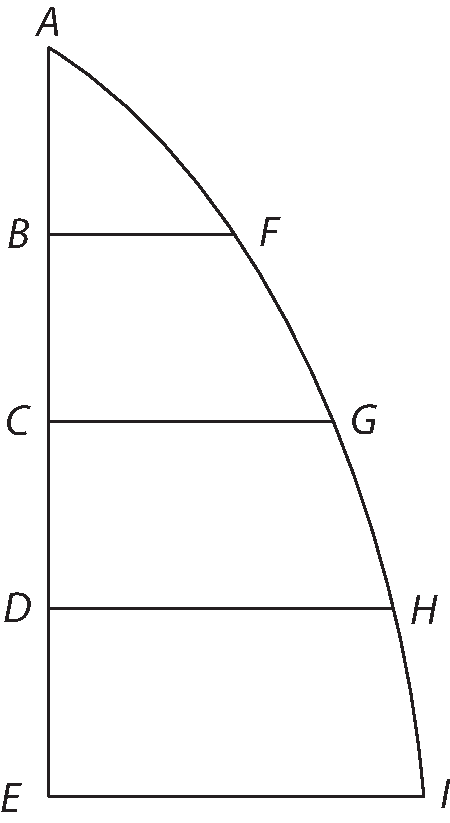
\includegraphics[width=0.3\textwidth]{images//LH035,14,02_139v-d.pdf}
%\noindent \centering [\textit{Fig. ??}]
%\end{wrapfigure}
 et nix corpori ampullae circumdetur, initio ascendit aqua usque ad $E$ supra $D$, deinde rursum descendet in $D$ et tandem rursus ascendet \edtext{etiam}{\lemma{}\Bfootnote{etiam \textit{erg.} \textit{L}}} supra $E$ paradoxum sed \edtext{verum.}{\lemma{verum.}\Cfootnote{a.a.O.\cite{00044}, S. 631.}} Ratio prioris experimenti haec est, quod scilicet initio tantum pars, subtilissimus nempe mercurius\protect\index{Sachverzeichnis}{mercurius} calore\protect\index{Sachverzeichnis}{calor} rarefit, et ascendit solus, atque \edtext{ita suam aquam}{\lemma{ita}\Bfootnote{\textit{(1)}\ vas \textit{(2)}\ suam aquam \textit{L}}} crescere et descendere sinit, at si calor longius duret rarefactio\protect\index{Sachverzeichnis}{rarefactio} rursus pertingit in totam aquam (+ et mercurium in eam recidit ambientis forte condensatione\protect\index{Sachverzeichnis}{condensatio} unde aliud in clausis Thermometris\protect\index{Sachverzeichnis}{thermometer} NB. +)
 \edtext{Sed haec ratio nulla est teste autore, quia si convexitas sit intrinseca prius ascendit. Ergo a vitro.}{\lemma{}\Bfootnote{Sed [...] vitro. \textit{erg.} \textit{L}}} Secundi experimenti alia plane ratio \edtext{est,}{\lemma{est,}\Cfootnote{a.a.O.\cite{00044}, S. 630.}} quod scilicet densatur vitrum, unde contrahitur, sphaera seu ampulla (introrsum), ergo et spatium, ergo \edtext{aqua}{\lemma{}\Bfootnote{aqua \textit{erg.} \textit{L}}} \edtext{altius ascendit}{\lemma{altius}\Bfootnote{\textit{(1)}\ ex \textit{(2)}\ ascendit \textit{L}}} (nam si convexitas vitri\protect\index{Sachverzeichnis}{convexitas vitri} sit intrinseca, aqua primum subsidit). At cur mox in fine altius evadit, quia perennis ex nive mercurii\protect\index{Sachverzeichnis}{nis mercurii} fluvius in ampullam \edtext{per poros}{\lemma{}\Bfootnote{per poros \textit{erg.} \textit{L}}} subit, et ita explicat augetque humoris molem\protect\index{Sachverzeichnis}{moles humoris}. Nota hunc esse illum \edtext{mercurium}{\lemma{mercurium}\Cfootnote{a.a.O.\cite{00044}, S. 631f.}} qui aquam frigefacit aestivam, aerem hybernum, qui saepe \textit{si fervente aestu pori laxiores, sanguinem} subito figit. 
\textit{Hinc aqua cocta ubi deferbuit salubrior.} (+ NB. hic \edtext{est meum}{\lemma{est}\Bfootnote{\textit{(1)}\ meus \textit{(2)}\ meum \textit{L}}} Alcali\protect\index{Sachverzeichnis}{alcali} summum seu Alcahest\protect\index{Sachverzeichnis}{Alcahest Helmontianum} Helmontianum. +) 
\textit{Hic mercurio subtilitatem et perpetuam fluiditatem conciliat, hinc
\edtext{aquae stygiae}{\lemma{aquae}\Bfootnote{\textit{(1)}\ \textit{frigidae} \textit{(2)}\ \textit{stygiae} \textit{L}}}
mortale frigus, hinc cicutae venenum\protect\index{Sachverzeichnis}{venenum} frigidum,
hinc aqua frigida ubi primum soli exponitur, frigidior sentitur,
quia primus ille calor subtilem hunc Mercurium\protect\index{Sachverzeichnis}{mercurius} excitat,
unde particulae quasi audaciores evadunt, et immersam manum}
\edtext{pene}{\lemma{pene}\Cfootnote{\textit{fere} in Vorlage.}}
\edtext{penetrant}{\lemma{penetrant}\Cfootnote{a.a.O.\cite{00044}, S.~630 mit Auslassung: \textit{frigidum,} [...] \textit{hinc}.}} (+ an ut modico humore augetur ignis, et mane oriente sole frigus majus +).
\textit{Hinc aqua ubi deferbuit saeviente bruma\protect\index{Sachverzeichnis}{bruma} citius} gelatur, discursus enim hujus humoris impedit \edtext{gelationem.}{\lemma{gelationem.}\Cfootnote{a.a.O.\cite{00044}, S.~630.}} In vitro poros esse vel hinc patet quod quaedam ex vitro hermetice sigillato modico calore \edtext{avolant.}{\lemma{avolant.}\Cfootnote{a.a.O.\cite{00044}, S. 632.}} \textit{Imo aliqui ipsum Mercurium metallicum quadam arte per poros vitrei vasis intrudunt. Adde si vis subtilem illum halitum vel succum ex aurei mali cortice\protect\index{Sachverzeichnis}{cortex mali} levi manu expressum, qui per poros vitrei scyphi intruditur. Quod si \edtext{dicas}{\lemma{dicas}\Cfootnote{a.a.O.\cite{00044}, S. 632.}}} irrepere per superficiem totam per vas superius coactum dices, non enim apparet in superioribus vestigium et idem est in Hermetice clausis.
\pend
\pstart Glacies\protect\index{Sachverzeichnis}{glacies} est densior aqua in partibus singulis, etsi totum sit rarius, hinc \edtext{partes glaciei tritae}{\lemma{partes}\Bfootnote{\textit{(1)}\ aquae \textit{(2)}\ glaciei tritae \textit{L}}} fundum petunt.
\pend 
\pstart Optimus Thermometri\protect\index{Sachverzeichnis}{thermometrum} modus hic est. Sit vas aqua plenum ampullae cujusdam aliquid aquae continentis longius collum inversum immergatur, quae aqua in subjectum vas non \edtext{defluet.}{\lemma{defluet.}\Cfootnote{a.a.O.\cite{00044}, S. 632.}} Aliud Thermometrum spiritu vini\protect\index{Sachverzeichnis}{spiritus vini} infuso, qui (contra quam aqua) calore ascendit, frigore \edtext{descendit.}{\lemma{descendit.}\Cfootnote{a.a.O.\cite{00044}, S. 635.}}
[138~r\textsuperscript{o}]
\pend%
\pstart%
%
%
%
% \input{gesamttex/edit/LH035_14_02_138r.tex}
% [138~r\textsuperscript{o}]
\textit{Aer non gravitat nisi vel habeat corpus rarius infra se, vel diversis partibus ejusdem plani aquae inaequaliter \edtext{incumbat.}{\lemma{incumbat.}\Cfootnote{a.a.O.\cite{00044}, S. 636.}}} Nam si plano aquae aer incumbat rarior, et \edtext{proinde minor}{\lemma{proinde}\Bfootnote{\textit{(1)}\ major \textit{(2)}\ minor \textit{L}}} hic reliqua descendens \edtext{aquam huc faciet attolli hic et deprimi}{\lemma{aquam}\Bfootnote{\textit{(1)}\ deprimet \textit{(2)}\ huc [...] deprimi \textit{L}}} illic. Luna\protect\index{Sachverzeichnis}{luna} autem aerem rarefacit (+ NB. posset hoc experimento quodam declarari. +)
\pend 
\count\Bfootins=1400
\count\Cfootins=1400
\pstart \textso{Hon. Rab. Tract. Phys. 2. append. cap. 2.} Nuper quaedam experimenta inventa, de quibus et Timaei Locrensis id est
Thomae \edtext{Cornelii Epistolam}{\lemma{}\Bfootnote{Cornelii \textbar\ Consentina \textit{gestr.}\ \textbar\ Epistolam \textit{L}}}\protect\index{Namensregister}{\textso{Cornelio}, Tommaso 1614-1686} legi. Est is calaber\protect\index{Sachverzeichnis}{calaber}, Medicus arte, sed aliquantum maledicus. Prodiit et quoddam Raph. Magiotti\protect\index{Namensregister}{\textso{Magiotti}, Raffaello 1597-1656} scriptum. Experimenta huc redeunt, 
\textit{si ampulla aere plena inverso situ immergatur aquae,
aer inclusus comprimitur.
Hinc quo \edtext{altius}{\lemma{altius}\Cfootnote{a.a.O.\cite{00044}, S.~637 mit Auslassungen:
\textit{ampulla} [...] \textit{aere plena} [...] \textit{inverso} und \textit{comprimitur.} [...] \textit{Hinc}.}}} descendit, major compresso, et plus aquae intrat. \textit{Hinc si vel digito vel alio modo post intrusionem aquae foramen obstruatur, eductoque globulo aperiatur ab aere compresso aqua foras extruditur, ut et}
\textit{Timaeus \edtext{observavit.}{\lemma{observavit.}\Cfootnote{a.a.O.\cite{00044}, S. 638.}}} Porro \textit{intrusa aqua et compresso incluso aere, si foramen obstruatur, inde gravior globulus \edtext{efficitur}{\lemma{efficitur}\Cfootnote{a.a.O.\cite{00044}, S.~638 mit Auslassung: \textit{foramen} [...] \textit{obstruatur}.}}} (+ NB. NB. +) et globus post hanc compressionem gravior fundum petere potest. (+ Hinc potest fieri motus perpetuus. +) Globuli \textit{collum \edtext{exile}{\lemma{}\Bfootnote{\textit{exile} \textit{erg.} \textit{L}}} deorsum vergat,} et allegari debet, ut in hoc situ teneatur \textit{frustulum laminae plumbeae\protect\index{Sachverzeichnis}{laminae plumbeae} vel aeris} observante Magiotto\protect\index{Namensregister}{\textso{Magiotti}, Raffaello 1597-1656}
debet hic globus esse 
\textit{paulo levior aqua,} ut parva accessione deprimatur, unde \textit{vel vitrum debet esse crassius vel} plumbo alligato ad collum gradus temperare, \textit{vel aqua immitti, quae sine vi extrudi non \edtext{possit,}{\lemma{possit,}\Cfootnote{a.a.O.\cite{00044}, S. 638.}}} quod fiat si globus incalescens in frigidam mittatur. Sit jam cavus cylinder aqua plenus, sit globulus summissus levior aqua, sed qui minima ponderis accessione gravior factus fundum petat, sigilletur cylinder hermetice. \edtext{Manus}{\lemma{}\Bfootnote{Manus \textit{erg.} \textit{L}}} calida cylindro admoveatur, descendit globus. Quidam rationem reddunt, quod aqua calore rarefacta levior. Sed hoc nihil, quia rarefactum fit levius quando rarescens explicatur, quod hic non. (+ mala objectio. Fit levius quia ignis explosionibus attollitur. +) Fit ergo gravior globus quia \textit{aqua calore rarefacta et intra \edtext{vas}{\lemma{vas}\Cfootnote{a.a.O.\cite{00044}, S. 638.}}} compressa plus aquae intrudit, unde \edtext{globus gravior}{\lemma{globus}\Bfootnote{\textit{(1)}\ levior \textit{(2)}\ gravior \textit{L}}} \edtext{(+\phantom)\hspace{-1.2mm} at}{\lemma{(+}\Bfootnote{\textit{(1)}\ et \textit{(2)}\ at \textit{L}}} ipse fassus si non firmetur non descendere. Imo etiam non firmatus descendit videtur utraque ratio eodem recidere +). Aqua restituta extensioni priori resurgit. Utraque ratio concurrit, quod scil. tantum extrudatur aqua quantum intruditur globo. Porro non esse in causa quod sola aqua sit rarefacta patet, quia clausus globus non ideo descendit (+~NB~[+]). Contra si globus tantulo sit brevior, ut \edtext{minima ponderis retractione emergat, corpore frigido}{\lemma{minima}\Bfootnote{\textit{(1)}\ frigore \textit{(2)}\ ponderis [...]
 frigido \textit{L}}} admoto, ascendet, ob eandem causam. Sed si nix vel glacies cylindro admoveatur etiam descendet, ut dictum supra ob emissionem mercurii\protect\index{Sachverzeichnis}{emissio mercurii} frigidi, mox rursum ascendet, inde rursum descendet durante diu \edtext{frigore.}{\lemma{frigore.}\Cfootnote{a.a.O.\cite{00044}, S. 639f.}} 
\textit{Si Tubus sit apertus, aqua plenus, immisso embolo,\protect\index{Sachverzeichnis}{embolum}
qui recte cum concavitate tubi conveniat, comprimatur aqua, globulus descendit,
quia facilius comprimitur aer globulo inclusus quam aqua, unde aqua in globulum intruditur.
Unde globus \edtext{gravior.}{\lemma{gravior.}\Cfootnote{a.a.O.\cite{00044}, S.~640 mit Auslassung: \textit{apertus,} [...] \textit{aqua}.}}} Idem si vel digito aquam premas, aut si os\protect\index{Sachverzeichnis}{os} admoveas ori canalis, quasi edicturus globulo $D$ ut deorsum eat, modico anhelitu \textit{aut si superior tubi pars utri alligata sit, quem leviter premas vel \edtext{stringas.}{\lemma{stringas.}\Cfootnote{a.a.O.\cite{00044}, S. 640.}}} Aqua \edtext{alio quia?}{\lemma{}\Bfootnote{alio \textbar\ aurii \textit{erg. u. gestr.}\ \textbar\ quia? \textit{L}}} proprie comprimi non potest, et globus aureus aqua plenus non potest comprimi quaecunque vis mechanica applicetur[;]
\textit{si intra vas aeneum aquam comprimere tentes per intrusionem aeris ut fieri \edtext{solet, frigidiorem senties,}{\lemma{senties,}\Cfootnote{a.a.O.\cite{00044}, S. 641 mit Auslassung: \textit{solet,} [...] \textit{frigidiorem}.}}} extrusis mercurialibus corpusculis, idque \edtext{probat trajectionem per poros vitri}{\lemma{probat}\Bfootnote{\textit{(1)}\ tractio \textit{(2)}\ trajectionem per poros vitri \textit{L}}} porro contra educto embolo et facta rarefactione, levabitur globus. 
\pend 
\pstart Similiter globus descendit si comprimas aerem qui est in vase clauso, si non ut priore casu, est totum aqua plenum, contra si dilates ascendit, si sit tubus aqua plenus, sint supra et infra duo exigua foramina acicula obstruibilia, natet globus \textit{instar exiguae ampullae partim aere partim aqua plenus, ita temperatus, ut tantum non supernatet, ac proinde descendat, volo nempe a tenuissimo reticulo retineri, ne deorsum \edtext{eat.}{\lemma{eat.}\Cfootnote{a.a.O.\cite{00044}, S. 643.}}} Utroque foramine obstructo globulus immotus manet. Aperto foramine superiori fit gravior, erat enim aqua prius supra affixa metu vacui, nunc deorsum gravitat aperto inferiore, cessat compressio aeris inclusio globuli, et levior evadit, ideoque ascendit quia scil. aliorsum jam aqua gravitat id est in foramen aerem subjectum. Si utrumque foramen aperiatur, \edtext{subsistit, nulla sequetur mutatio}{\lemma{subsistit,}\Bfootnote{\textit{(1)}\ ubi erat \textit{(2)}\ nulla sequetur mutatio; \textit{L}}}; Mallem autem esse basin vitream quam \edtext{coriaceam.}{\lemma{coriaceam.}\Cfootnote{a.a.O.\cite{00044}, S. 643f.}}
Si tubus sit tantum infra obstructus, rarescens calore faciet ascendere globum, frigus
\edtext{descendere, quia aer}{\lemma{descendere,}\Bfootnote{\textit{(1)}\ et si mercurii \textit{(2)}\ quia aer \textit{L}}} inclusus densatusque aquam exugit (+ NB. Ergo aer potius exugit aquam quam illa aerem, ergo est subjectum compressionis et rarefactionis ut in thermometro +). Etsi mercurius ille frigidus admoveatur nil mutat tamen, quia exire rursus per foramen
\edtext{potest.}{\lemma{potest.}\Cfootnote{a.a.O.\cite{00044}, S. 644.}} Duobus globulis \edtext{in vas apertum}{\lemma{}\Bfootnote{in vas apertum \textit{erg.} \textit{ L}}} immissis rarefactione apertus ascendit, clausus \edtext{manet. At}{\lemma{manet.}\Bfootnote{\textit{(1)}\ Et contra sive clausum sit vas sive non \textit{(2)}\ At \textit{L}}} in refrigeratione per superiora distingue, si vas supra apertum frigido admoto ille \edtext{descendit quia aer}{\lemma{descendit quia}\Bfootnote{\textit{(1)}\ aqua \textit{(2)}\ aer \textit{L}}} inclusus condensatur,
hic \textso{clausus} ascendit, quia aqua \edtext{densatur. Si}{\lemma{}\Bfootnote{densatur. \textbar\ NB. (+ Aquae ergo densatio levat non rarefactio demittit. +) \textit{gestr.}\ \textbar\ Si \textit{L}}} vas sit obstructum, et uterque globus supernatet admoto calido uterque descendet, apertus ob intrusam
aquam, \textso{clausus} ob medium factum rarius. Admoto frigido fieri potest ut apertus descendat, clauso innatante, si frigidum mercurium\protect\index{Sachverzeichnis}{mercurius frigidus} quendam emittet, aquam intrusione sin comprimentem Globus supernatans aegre, percusso valide vase descendet, quia aere ictu\protect\index{Sachverzeichnis}{ictus} ex globulo eliso, aqua succedet. Compresso ore tubi apertus immergetur, non obstructus (+ quia hunc impedit potius aquae densatio NB +). 
\textit{Duo globuli erant in scypho, aqua pleno, alter frigescente aqua emergebat et calescente immergebatur; alter frigescente immergebatur, et calescente emergebat. Primus erat obstructus,} sed ita ut esset aqua rarescente gravior, et condensata levior paulo,
\textit{secundus exiguo foramine patebat, ita compositus, ut per accessionem modicae gravitatis\protect\index{Sachverzeichnis}{gravitas modica} immergeretur, detractionem \edtext{emergeret.}{\lemma{emergeret.}\Cfootnote{a.a.O.\cite{00044}, S. 645.}}}
\pend
\count\Bfootins=1200
\count\Cfootins=1200
\pstart
De palulis cereis ferrea scobe temperatis vid. tr. de Elementis de 
\edtext{liquore}{\lemma{liquore}\Cfootnote{\textsc{H. Fabri}, \title{Physica}\cite{00044}, Bd. 2, Lyon 1670, Trakt. 5, Buch 2.}} supra libellum per canaliculum utrinque apertum ascendente vid. dict. tr. et dial. de globis aqueis et \mercury\textsuperscript{ii} de ampullis, figura flammae\protect\index{Sachverzeichnis}{figura flammae}, dictis 
\edtext{locis.}{\lemma{locis}\Cfootnote{\textsc{H. Fabri}, \title{Dialogi physici}\cite{00187}, Lyon 1665, S. 218-220, 179f., 162-165; \textsc{Ders.},
 \title{Physica}\cite{00044}, Bd. 1, Lyon 1669, S. 645f.}} 
Adde \mercury\ in tubo libratum et alia quae \textit{exhausimus tum in appendice ad meta\pgrk{f}ysicam de vacuo, tum in dialogis, item vim Electricam \edtext{quae}{\lemma{quae}\Cfootnote{a.a.O.\cite{00044}, S.~646.}}} et ipsa a tensione et compressione pendet. Fateor desiderari quaedam \textit{ad progressionem illorum motuum pertinentia, qui ex tensione et compressione sequuntur. Et plena integra tractatio deest de chordarum et arcuum reductione de \mercury\textsuperscript{\textit{ii}} librationibus, et multis aliis quae in singularem tractatum referemus licet enim de motu \edtext{locali}{\lemma{locali}\Cfootnote{\textsc{H. Fabri} (Petrus Mosnerius), \title{Tractatus physicus de motu locali}\cite{00307}, Lyon 1646.}} \edtext{corporum}{\lemma{corporum}\Cfootnote{\textsc{H. Fabri}, \title{Physica}\cite{00044}, Bd. 1, Lyon 1669, S.~646.}}} egerimus plurima tamem restant, \textit{ut nonnulla a Mousnerio \protect\index{Namensregister}{\textso{Mousnerius}, Petrus}
astructa explicentur et emendentur, quod in meta\pgrk{f}ys. magnam partem praestitum, tum ut alia omissa addantur circa tensa, compressa librata, vibrata, projecta, tracta impacta justum \edtext{volumen}{\lemma{volumen}\Cfootnote{a.a.O.\cite{00044}, S.~646.}}} de his jam fere affectum habemus, quod \pgrk{F}ysicam sequetur. Unde satius dixi universam de motu tractationem in unum congerere quam membratim \edtext{discerpere.}{\lemma{discerpere.}\Cfootnote{a.a.O.\cite{00044}, S.~646.}}
[158~v\textsuperscript{o}]
\pend%
\pstart%
%
%
%
% \input{gesamttex/edit/LH035_14_02_158v.tex}
% [158~v\textsuperscript{o}]
\textso{Hon. Fab. Tract.} \pgrk{F}\,\textso{ys. 2. append. cap. 2. n. }\edtext{[\textso{13}]}{\lemma{}\Bfootnote{\textso{15}
\textit{\ L \"{a}ndert Hrsg. }}}\textso{ sqq.}
\textit{Circa Mercurium\protect\index{Sachverzeichnis}{mercurius} tubo contentum novum experimentum a }\textit{Fabricio Guastaferro}\protect\index{Namensregister}{\textso{Guastaferri}, Fabrizio}\textit{ inventum est. Sit canaliculus valde angustus, sex palmos longus, apertus hinc, illinc clausus, immittatur \mercury\ ad 4 palmos, vel minus, sed probe purgatus a pulvere scoria et aliis \edtext{faecibus,}{\lemma{faecibus,}\Cfootnote{a.a.O.\cite{00044}, S. 646.}}} invertatur Tubus, sistet mercurius nec descendet infra 4 palmos, si vero immittatur ad 5 palmos tunc jam fortior \edtext{M.}{\lemma{M.}\Cfootnote{Mercurius.}} ultra descendet et supra spatium relinquet quia scilicet tunc \edtext{superat pondere materiam subtilis materiae}{\lemma{superat}\Bfootnote{\textit{(1)}\ resistentiam subtilis ma \textit{(2)}\ pondere [...] materiae \textit{L}}} tendendae et educendae. Hinc si tubus latior non sistit in 4 palmis, quia divisio facilior.
\textit{Idem aquae accidit in angustioribus canalibus propter eandem rationem quomodo aqua per spiras descendat intra tubum, dum aera sursum trudit, explicuimus tr. de \edtext{Elementis}{\lemma{Elementis}\Cfootnote{\textsc{H. Fabri}, \title{Physica}\cite{00044}, Bd. 2, Lyon 1670, Trakt. 5, Buch 2.}} et in \edtext{dialogis.}{\lemma{dialogis.}\Cfootnote{\textsc{H. Fabri}, \title{Dialogi physici}\cite{00187}, Lyon 1665, S.~54. \textsc{Ders.},
\title{Physica}\cite{00044}, Bd.~1, Lyon 1669, S.~646.}}} Porro si Tubus paulum \textit{succutiatur mercurii ultima basis relinquit fundum \edtext{tu}{\lemma{tubi}\Cfootnote{a.a.O.\cite{00044}, S. 646.}} \hspace{-1.2mm}\edtext{bi.}{\lemma{}\Bfootnote{\textit{tubi} \textbar\ \textit{et accidit} \textit{gestr.}\ \textbar\ .  Sed \textit{L}}}}
Sed mox motu accelerato restituitur. Si non sit probe purgatus non sistit, quia aer per rimas a scoria apertas transit. Si Mercurio\protect\index{Sachverzeichnis}{mercurius} superfundatur \textit{aqua, quae occupet spatium ante ab aere \edtext{occupatum,}{\lemma{occupatum,}\Cfootnote{a.a.O.\cite{00044}, S. 647.}}} et invertatur tubus ut supra descendit omnino, mercurius et sursum extruditur aqua. Ratio hujus praeclari experimenti, quia \textit{aer tantulum compressus premit extremum limbum basis mercurii ut eam in convexum tornet, ut fuse in
\edtext{dialogis.}{\lemma{dialogis.}\Cfootnote{\textsc{H. Fabri}, \title{Dialogi physici}\cite{00187}, Lyon 1665, 4. Dialog.}}}
\textit{Quid mirum ergo si per medium}
\mercury\textsuperscript{\textit{ium}}\textit{ non
\edtext{eat,}{\lemma{eat,}\Cfootnote{\textsc{H. Fabri}, \title{Physica}\cite{00044}, Bd. 1, Lyon 1669, S. 647.}}} at aqua quippe non compressa non tendit versus extremitates, sed \textit{longe facilius per medium \mercury\textsuperscript{\textit{ium}}
\edtext{ascendit.}{\lemma{ascendit.}\Cfootnote{a.a.O.\cite{00044}, S. 647.}}} Si aqua non mercurius sit 
\edtext{in \textit{inverso}}{\lemma{}\Bfootnote{in \textbar\ tubo \textit{gestr.}\ \textbar\ \textit{inverso} \textit{ L}}} \textit{tubo statim aqua descendit et aera sursum extrudit, quia aeris pressio in basin aquae superiorem convexitatem non 
\edtext{inducit. Sed ut}{\lemma{inducit.}\Bfootnote{\textit{(1)}\ \textit{Idem de} \textit{(2)}\ \textit{Sed ut} \textit{L}}} in dialogis demonstravi 
\edtext{concavitatem}{\lemma{concavitatem}\Cfootnote{\textsc{H. Fabri}, \title{Dialogi physici}\cite{00187}, Lyon 1665, S. 102-104.}}, unde extrusio aeris per \edtext{medium facilior.}{\lemma{facilior.}\Cfootnote{\textsc{H. Fabri}, \title{Physica}\cite{00044}, Bd. 1, Lyon 1669, S. 647 mit Auslassung: \textit{medium} [...] \textit{facilior.}}}} Idem de aliis liquoribus excepto solo 
\mercury\ 
\textsuperscript{io}. Si missus mercurius in canalicum \edtext{occupet dictum spatium}{\lemma{occupet}\Bfootnote{\textit{(1)}\ dictos 4 palmos \textit{(2)}\ dictum spatium \textit{L}}} mittatur
\textit{in eum filum ferreum\protect\index{Sachverzeichnis}{filum ferreum} gossypio\protect\index{Sachverzeichnis}{gossyps} instructum quasi ad instar Emboli, ubi deinde retrahitur filum, ne detur vacuum mille aeris particulae intra gossypium latentes eductae tenduntur et dilatantur ad oculum\protect\index{Sachverzeichnis}{oculus} a quibus deinde filum ipsum trahitur dum illae se reducunt jucundum experimentum, cujus praeter \edtext{assignatum}{\lemma{assignatum}\Cfootnote{a.a.O.\cite{00044}, S. 647.}}} ratio nulla. Si pro more vulgaris experimenti admoveas digitum, inter invertendum, et immergas in mercurium\protect\index{Sachverzeichnis}{mercurius} vase supposito mercurius descendit, et extat supra palmorum
\rule[-4mm]{0mm}{10mm}$\displaystyle4\frac{1}{3}$
circiter, pro mensura priori. Jam si admoto denuo digito magno impetu tubum invertas, mox deorsum magno impetu nec suspensus manet. In \edtext{dialogis}{\lemma{dialogis}\Cfootnote{a.a.O.\cite{00044}, S. 647.}} etiam ex eo probavimus mercurium ab aere non sustineri, quia pondus mercurii sentitur a sustinente fistulam vitream\protect\index{Sachverzeichnis}{fistula vitrea} (+ NB +) Eorum responsione rejecta qui sibi persuaserant \mercury\textsuperscript{ium} in tubi latera gravitare, venit ex eo in manus meas aureum \textit{Doctissimi Famiani Michelini}\protect\index{Namensregister}{\textso{Michelini}, Famiano 1604-1665}
\textit{opusculum de fluminum directione, ubi idem prorsus adstruit de aquis alveo seu vase contentis, si enim alvei latera\protect\index{Sachverzeichnis}{latera alvei} seu parietes erecti sint perpendiculariter, et probe levigati, nulla aut modica vis ponderis in eos gravitat, modica \edtext{sane.}{\lemma{sane.}\Cfootnote{a.a.O.\cite{00044}, S. 648.}}} Nam gravitatio in fundum est ad gravitationem in latus tunc \edtext{ut superficies}{\lemma{ut}\Bfootnote{\textit{(1)}\ gravitas \textit{(2)}\ superficies \textit{L}}} ad 
\edtext{lineam. Aer non potest Mercurium}{\lemma{lineam.}\Bfootnote{\textit{(1)}\ Si me \textit{(2)}\ Aer non potest Mercurium \textit{L}}} sustinere nisi sustinendo superficiem seu fundum inferioris \textit{mercurii vase contenti. Ergo qui fistulam erectam tenet, nullum \mercury\textsuperscript{\textit{ii}}\protect\index{Sachverzeichnis}{mercurius} pondus \edtext{sentiret.}{\lemma{sentiret.}\Cfootnote{a.a.O.\cite{00044}, S. 648 mit Auslassung: \textit{contenti.} [...] \textit{Ergo}.}}}
\pend%
\count\Afootins=1500
\count\Bfootins=1500
\count\Cfootins=1500
%
%%%%% ENDE